\documentclass[14pt]{extreport}
\usepackage{cmap} % copy from pdf
\usepackage[T2A]{fontenc} 
\usepackage[utf8x]{inputenc} 
\usepackage[english,russian]{babel} 
\usepackage{
  amssymb,
  amsfonts,
  amsmath,
  mathtext,
  cite,
  enumerate,
  float,
  amsthm} 
\usepackage{hyperref} % for url in bibtex

% \renewcommand\qedsymbol{${\mathlarger \blacktriangleright }$}
% \renewcommand\qedsymbol{\textbf{QED}}
 
\newtheorem{definition}{Определение}[section] 
\newcommand{\bra}[1]{\left\langle #1 \right|}
\newcommand{\ket}[1]{\left| #1 \right\rangle}
\newcommand{\p}[1]{\left( #1 \right)}

\usepackage{ragged2e} 
\usepackage{verbatim} % enviroment without latex
\usepackage{relsize} % {\mathlarger mathform}

% PAPER PARAMETERS
\usepackage{geometry} 
 \geometry{left=25mm} 
 \geometry{right=10mm} 
 \geometry{top=20mm} 
 \geometry{bottom=20mm} 

% containers for figure with [ht]
% \usepackage{float}
% pic
\usepackage[pdftex]{graphicx, xcolor} 
% filepath for pic
\graphicspath{{../figures}} 
% for subfigure
\usepackage{subcaption}

% help
\usepackage{lineno}
\linenumbers
\usepackage{xcolor}


\title{МНОГОЧАСТИЧНАЯ ЗАПУТАННОСТЬ В МНОГОКВАНТОВОЙ СПЕКТРОСКОПИИ ЯМР В ТВЕРДОМ ТЕЛЕ}
\author{Илья Лазарев}
\date{Последняя редакция: \today}

\begin{document}
\maketitle

\begin{titlepage}
% \begin{flushright}
%    Приложение № 5 \\
%    к Положению о диссертационном \\
%    совете Московского государственного \\
%    университета имени М.В.Ломоносова
% \end{flushright}
% \vspace{1cm}
\begin{center}
  {\large Московский государственный университет им. М.В. Ломоносова} \\
  {\it Факультет фундаментальной физико-химической инженерии} \\
  \vspace{1cm}
  {\large Институт проблем химической физики РАН} \\
  {\it Лаборатория спиновой динамики и спинового компьютинга} \\
  \vfill
  (на правах рукописи) \\
  \vfill
  {\Large \bf Лазарев Илья Дмитриевич} \\
  \vspace{1cm}
  {\Large \bf
      Многочастичная запутанность \\
      в многоквантовой спектроскопии ЯМР \\
      \vspace{2mm}
      в твердом теле
  }
 \vfill
  1.3.8 Физика конденсированного состояния \\
 \vspace{1cm}
 ДИССЕРТАЦИЯ \\
 на соискание ученой степени \\
 кандидата физико-математических наук
 \vfill
 {\large
   Научный руководитель:\\
   д.ф.-м.н. профессор Фельдман Эдуард Беньямиович
 }
 \vfill
 Москва, 2022 г.
\end{center}
\end{titlepage}
\addtocounter{page}{1}

\tableofcontents

%\raggedright  %отмена переносов
%\justify %выравнивание по ширине

% Во введении к диссертации определяется актуальность избранной темы, степень ее разработанности, цели и задачи, объект и предмет исследования, научная новизна, теоретическая и практическая значимость работы, методология диссертационного исследования, положения, выносимые на защиту, степень достоверности и апробация результатов.

\textbf{Актуальность темы исследования.}
Квантовые корреляции ответственны за преимущества квантовых приборов и устройств над их классическими аналогами.
Такие корреляции отсутствуют в классической физике.
Изучение их свойств и методов управления ими является теоретической основой квантовых технологий.

Традиционно такие корреляции связывают с понятием запутанности~\cite{Einstein1935},
но в квантовой теории информации существует и более общий класс квантовых корреляций --- квантовый дискорд~\cite{Bera2017}.
Квантовый дискорд отличен от нуля~\cite{Yurishchev2011} даже в отсутствии запутанности и при высоких температурах,
тем не менее основным ресурсом
квантовой информатики~\cite{Arute2019},
квантовой криптографии~\cite{Gisin2002},
метрологии~\cite{Toth2012}
и коммуникации~\cite{Yin2017}
является запутанность.
Изучение этого ресурса --- одна из актуальнейших проблем квантовой теории информации~\cite{Nielsen2010}.
Предпринятые в данной работе попытки количественного определения многочастичной запутанности мотивированы
желанием понять и количественно оценить эти ресурсы.


С фундаментальной точки зрения большой интерес вызывают квантовые процессы,
протекающие в системах многих взаимодействующих частиц,
например, термализация~\cite{DAlessio2016}, скремблирование~\cite{Hosur2016},  локализация~\cite{Alvarez2010}.
Являясь характерной особенностью квантовой механики~\cite{Schrodinger1935},
запутанность оказывается~\cite{Kaufman2016, Neill2016, Garttner2018} ключевой особенностью этих процессов.
Дальнейшее исследование таких процессов
требует развития экспериментальных методов исследования многочастичной запутанности.
До недавнего времени исследования~\cite{Horodecki2009} были ограничены изучением запутанности
и квантового дискорда между двумя подсистемами
и направлены на определение мер этих величин.
Вместе с тем более существенны не меры квантовых корреляций,
а сам факт их наличия.
В последние годы возникли~\cite{Garttner2018} методы исследования многочастичной запутанности.
В частности, оказалось, что в рамках многоквантовой (МК) спектроскопии ЯМР в твердом теле можно существенно продвинуться в этом направлении.

% С фундаментальной точки зрения запутанность является ключевой концепцией квантовой механики~\cite{},
% и например недавно была предложена~\cite{DAlessio2016} и экспериментально проверена~\cite{Kaufman2016, Neill2016} теория термализации изолированных квантовых систем на основе квантовой запутанности.
% Также запутанность~\cite{Ball2011} фигурирует в ряде естественных биологических процессов.
% В настоящее время запутанность является базовым инструментом для изучения экспериментов распада частиц~\cite{Bernabeu2012}.
% Также было обнаружено~\cite{Ball2011}, что запутанность фигурирует в ряде естественных биологических процессов.

% % Например, продемонстрированная~\cite{Arute2019} командой Google заявка на квантовое превосходство
% % полученное на программируемом сверхпроводящем процессоре
% % обеспечивается запутанностью.
% % Продемонстрированная~\cite{YIN2017} китайской группой передача квантовых состояний между искусственным космическим спутником и Землей реализована на основе запутанных состояний.
% % В ряде экспериментов распада частиц, как в работе\cite{Bernabeu2012} демонстрирующую асимметрию времени для субатомных процессов,
% % запутанность используется как инструмент удалённого измерения частицы.
% и например недавно была предложена~\cite{DAlessio2016} и экспериментально проверена~\cite{Kaufman2016, Neill2016} теория термализации изолированных квантовых систем на основе квантовой запутанности.
% Также запутанность~\cite{Ball2011} фигурирует в ряде естественных биологических процессов.



% \textbf{Степень ее разработанности.}
% JETP-2018
МК спектроскопия ЯМР~\cite{Baum1985} уже много лет известна как эффективный метод изучения корреляций многих взаимодействующих частиц,
так как на подготовительном периоде МК эксперимента ЯМР~\cite{Baum1985} создаются многоспиновые коррелированные кластеры.
% Главным образом МК ЯМР позволяет создавать многоспиновые коррелированные кластеры.
В работах~\cite{Krojanski2004, Zobov2006, Cho2006, Bochkin2018} были исследованы процессы роста таких коррелированных кластеров и зависимости времени декогеренции от их размера.
Также была отмечена связь запутанности с эволюцией МК когерентностей~\cite{Doronin2003, Furman2008}, %Furman2009},
а в работах~\cite{Feldman2008, Feldman2012} были введены свидетели двухчастичной запутанности.
Позднее метод МК ЯМР был применен для исследования эффекта локализации~\cite{Wei2018}.%~\cite{Alvarez2010, Alvarez2013, Alvarez2015, Wei2018}.

В недавней работе Гарттнер и др. показали~\cite{Garttner2018},
что специфический класс корреляторов,
первоначально разработанных в рамках МК спектроскопии ЯМР~\cite{Baum1985},
является полезным свидетелем многочастичной запутанности.
Спектр интенсивностей МК когерентностей ЯМР,
детектируемый по окончанию МК эксперимента ЯМР~\cite{Baum1985},
позволяет оценивать величину квантовой информации Фишера,
которая, в свою очередь, связана~\cite{Toth2014} с количеством запутанных частиц в системе.

Существуют и другие методы детектирования~\cite{Guhne2009} многочастичной запутанности.
В частности, критерий на основе энтропии Реньи~\cite{Hosur2016, Fan2017}
является строгим свидетелем многочастичной запутанности для чистых состояний.
Энтропия Реньи может быть измерена экспериментально,
но для этого требуются ресурсы,
которые экспоненциально масштабируются с размером изучаемой системы,
а также возможность одночастичной адресации.
Развиваемый в данной работе критерий многочастичной запутанности на основе МК спектра ЯМР
также является экспериментально доступным~\cite{Baum1985} свидетелем запутанности,
но менее требовательным к ресурсам,
а также применимым как к открытым,
так и к изолированным квантовым системам.


% \textbf{Цели и задачи.}
\textbf{Целью данной работы} является теоретическое исследование многочастичной запутанности в системах с большим количеством частиц $(>200)$ в рамках МК спектроскопии ЯМР,
а также развитие методов экспериментального измерения величин квантовой информации Фишера и косой информации Вигнера-Янасе.

% \textbf{Задачи:}
% \begin{enumerate}
%   \item Разработать теорию МК ЯМР для системы эквивалентных спинов при произвольной температуре.
%   \item Исследовать температурную зависимость многочастичной запутанности в нанопоре.
%   \item Исследовать температурную зависимость многочастичной запутанности в нанопоре с дипольно упорядоченным начальным состоянием.
%   \item Исследовать многочастичную запутанность в квазиодномерных цепочках ядерных спинов в зависимости от параметров цепи и температуры.
%   \item Провести сравнение оценок многочастичной запутанности, полученных на основе квантовой информации Фишера и косой информации Вигнера-Янасе.
% \end{enumerate}

\textbf{Научная новизна.}
В данной работе была разработана теория МК ЯМР для нанопоры при произвольной температуре,
что позволило впервые теоретически исследовать температурную зависимость многочастичной запутанности в системе из более чем 200 взаимодействующих частиц.
Также в данной работе был разработан метод определения величины косой информации Вигнера-Янасе в МК эксперименте ЯМР.

\textbf{На защиту выносятся следующие основные результаты и положения:}
\begin{enumerate}
  \item 
  Разработана теория МК ЯМР для системы эквивалентных спинов при произвольной температуре.
  
  \item 
  Исследована температурная зависимость многочастичной запутанности в нанопоре, 
  когда система приготовлена в термодинамическом равновесном зеемановском и дипольно упорядоченном состояниях.
  
  \item
  Исследована многочастичная запутанность в квазиодномерных цепочках ядерных спинов в зависимости от параметров цепи и температуры.
  
  \item 
  Предложен метод экспериментального измерения точного значения косой информации Вигнера-Янасе в рамках МК спектроскопии ЯМР.
  
  \item 
  Проведено сравнение оценок многочастичной запутанности, полученных на основе квантовой информации Фишера и косой информации Вигнера-Янасе.
\end{enumerate}
% \begin{enumerate}
%   \item Разработана теория МК ЯМР для системы эквивалентных спинов при произвольной температуре.
%   \item Исследована температурная зависимость многочастичной запутанности в нанопоре с термодинамическим и дипольно упорядоченным начальными состояниями.
%   \item Исследована многочастичная запутанность в квазиодномерных цепочках ядерных спинов в зависимости от параметров цепи и температуры.
%   \item Предложен метод экспериментального измерения точного значения косой информации Вигнера-Янасе в рамках МК спектроскопии ЯМР.
%   \item Проведено сравнение оценок многочастичной запутанности, полученных на основе квантовой информации Фишера и косой информации Вигнера-Янасе.
% \end{enumerate}

\textbf{Практическая ценность.}
Так как косая информация Вигнера-Янасе нашла много применений в квантовой теории информации, %~\cite{Wigner1963, Luo2017},
предлагаемый в данной работе метод определения ее величины
не только позволяет исследовать многочастичную запутанность методами МК ЯМР,
но и открывает возможность решения широкого класса задач в этой области.

\textbf{Публикации и апробация работы.}
Все результаты, представленные в диссертации,
опубликованы в высокорейтинговых зарубежных и российских научных журналах (Physical Review A, 2019;  Journal of Magnetic Resonance, 2020; Журнал экспериментальной и теоретической физики, 2020; Applied Magnetic Resonance, 2020;  Physics Letters A, 2021) и представлены на пяти международных и одной всероссийской конференциях.



% Многоквантовая (МК) спектроскопия ЯМР была введена для исследования распределения ядерных спинов в различных материалах (жидкие кристаллы, простые органические системы, аморфный гидрогенизированный кремний и т.д.).
% Он также оказался полезным для исследования скорости декогеренции в сильно коррелированных спиновых кластерах \cite{decoherence_register,decoherence_ca_f2}.
% Также была продемонстрирована зависимость скорости декогеренции от числа коррелированных спинов \cite{decoherence_register,lab:decoherence_2018}.
% По сути, динамика MQ ЯМР является подходящим методом для количественной оценки развития MQ когерентности, начиная с $z$-поляризации и заканчивая коллективным состоянием всех спинов.
% Метод позволяет описать распространение корреляций \cite{mq_nmr_experiment,spin_distribution_in_liquid_system,decoherence_under_dq,nmr_dyn} и предлагает сигнатуру эффектов локализации \cite{loc_deloc_nmr_dyn,loc_in_chain}. Скорость распространения может быть описана через вневременные упорядоченные корреляции (OTOCs), которые связаны с распределением когерентностей MQ ЯМР.
%

%
%
% В современной науке запутанность стала ключевым концептом квантовой механики.





%
%
% Nowadays, it has been recognized that most physical
% processes in nature can be formulated in terms of processing of information, and information may be central
% to understanding quantum theory [19].
%
%
% проблема классификации и количественной оценки запутанности в целом на сегодняшний день все еще далека от полного понимания.

% Such an investigation of many-spin entanglement is performed for the first time.

\documentclass[
    % notes,
    aspectratio=169
]{beamer}
\hypersetup{unicode=true} % fix "PD1 encoding, removing `\CYRI'"
\usepackage[utf8]{inputenc}
\usepackage[T2A,T1]{fontenc}
\usepackage[english,russian]{babel}

\usepackage{caption}
\usepackage{subcaption}

\graphicspath{{../figures}}

\newcommand{\tr}[1]{\mathrm{Tr} \left\{ #1 \right\}}
\newcommand{\sx}{I_\mathrm{x}}
\newcommand{\sy}{I_\mathrm{y}}
\newcommand{\sz}{I_\mathrm{z}}
\newcommand{\hdz}{H_\mathrm{dz}}


\setbeamertemplate{caption}[numbered] % number figures

\usetheme{Madrid}

\title[Многочастичная запутанность]{Многочастичная запутанность}
\subtitle{в многоквантовой спектроскопии ЯМР в твердом теле}
\author[Лазарев И.Д.]{\textbf{И.Д. Лазарев\inst{1,2}} \and  Э.Б. Фельдман\inst{2}}

\institute[МГУ, ИПХФ РАН]
{
  \inst{1}%
  Московский государственный университет им. М. В. Ломоносова
  \and
  \inst{2}%
  Институт проблем химической физики РАН
}

\date[2022]{Июнь 2022}


\begin{document}

\frame{\titlepage}
\note{
    Еще раз добрый день, коллеги!
    Я веду свою научную работу в Черноголовке
    в ИПХФ РАН в теоретическом отделе
    в лаборатории спиновой динамики и спинового компютинга
    под руководством Фельдмана Эдуарда Беньяминовича

    Тема моей работы: Многочастичная запутанность...

    Почему это важно?
    Квантовые корреляции ответственны за преимущества квантовых приборов и устройств над их классическими аналогами.
    Такие корреляции отсутствуют в классической физике.
    Изучение их свойств и методов управления ими является теоретической основой квантовых технологий.

    Почему ЯМР?
    Потомучто в твердотельном ЯМР можно значительно продвинуться в этом направлении.
}

% \AtBeginSection[] {} % show display table of contest before new section
\begin{frame}
\frametitle{План доклада}
\tableofcontents
\end{frame}
\note{
    В моем докладе будет две основные секции.
    Первая посвящена разбору задачи и методологии,
    а вторая полученным результатам.
}

\section{Введение}
% Во введении к диссертации определяется актуальность избранной темы, степень ее разработанности, цели и задачи, объект и предмет исследования, научная новизна, теоретическая и практическая значимость работы, методология диссертационного исследования, положения, выносимые на защиту, степень достоверности и апробация результатов.

\textbf{Актуальность темы исследования.}
Квантовые корреляции ответственны за преимущества квантовых приборов и устройств над их классическими аналогами.
Такие корреляции отсутствуют в классической физике.
Изучение их свойств и методов управления ими является теоретической основой квантовых технологий.

Традиционно такие корреляции связывают с понятием запутанности~\cite{Einstein1935},
но в квантовой теории информации существует и более общий класс квантовых корреляций --- квантовый дискорд~\cite{Bera2017}.
Квантовый дискорд отличен от нуля~\cite{Yurishchev2011} даже в отсутствии запутанности и при высоких температурах,
тем не менее основным ресурсом
квантовой информатики~\cite{Arute2019},
квантовой криптографии~\cite{Gisin2002},
метрологии~\cite{Toth2012}
и коммуникации~\cite{Yin2017}
является запутанность.
Изучение этого ресурса --- одна из актуальнейших проблем квантовой теории информации~\cite{Nielsen2010}.
Предпринятые в данной работе попытки количественного определения многочастичной запутанности мотивированы
желанием понять и количественно оценить эти ресурсы.


С фундаментальной точки зрения большой интерес вызывают квантовые процессы,
протекающие в системах многих взаимодействующих частиц,
например, термализация~\cite{DAlessio2016}, скремблирование~\cite{Hosur2016},  локализация~\cite{Alvarez2010}.
Являясь характерной особенностью квантовой механики~\cite{Schrodinger1935},
запутанность оказывается~\cite{Kaufman2016, Neill2016, Garttner2018} ключевой особенностью этих процессов.
Дальнейшее исследование таких процессов
требует развития экспериментальных методов исследования многочастичной запутанности.
До недавнего времени исследования~\cite{Horodecki2009} были ограничены изучением запутанности
и квантового дискорда между двумя подсистемами
и направлены на определение мер этих величин.
Вместе с тем более существенны не меры квантовых корреляций,
а сам факт их наличия.
В последние годы возникли~\cite{Garttner2018} методы исследования многочастичной запутанности.
В частности, оказалось, что в рамках многоквантовой (МК) спектроскопии ЯМР в твердом теле можно существенно продвинуться в этом направлении.

% С фундаментальной точки зрения запутанность является ключевой концепцией квантовой механики~\cite{},
% и например недавно была предложена~\cite{DAlessio2016} и экспериментально проверена~\cite{Kaufman2016, Neill2016} теория термализации изолированных квантовых систем на основе квантовой запутанности.
% Также запутанность~\cite{Ball2011} фигурирует в ряде естественных биологических процессов.
% В настоящее время запутанность является базовым инструментом для изучения экспериментов распада частиц~\cite{Bernabeu2012}.
% Также было обнаружено~\cite{Ball2011}, что запутанность фигурирует в ряде естественных биологических процессов.

% % Например, продемонстрированная~\cite{Arute2019} командой Google заявка на квантовое превосходство
% % полученное на программируемом сверхпроводящем процессоре
% % обеспечивается запутанностью.
% % Продемонстрированная~\cite{YIN2017} китайской группой передача квантовых состояний между искусственным космическим спутником и Землей реализована на основе запутанных состояний.
% % В ряде экспериментов распада частиц, как в работе\cite{Bernabeu2012} демонстрирующую асимметрию времени для субатомных процессов,
% % запутанность используется как инструмент удалённого измерения частицы.
% и например недавно была предложена~\cite{DAlessio2016} и экспериментально проверена~\cite{Kaufman2016, Neill2016} теория термализации изолированных квантовых систем на основе квантовой запутанности.
% Также запутанность~\cite{Ball2011} фигурирует в ряде естественных биологических процессов.



% \textbf{Степень ее разработанности.}
% JETP-2018
МК спектроскопия ЯМР~\cite{Baum1985} уже много лет известна как эффективный метод изучения корреляций многих взаимодействующих частиц,
так как на подготовительном периоде МК эксперимента ЯМР~\cite{Baum1985} создаются многоспиновые коррелированные кластеры.
% Главным образом МК ЯМР позволяет создавать многоспиновые коррелированные кластеры.
В работах~\cite{Krojanski2004, Zobov2006, Cho2006, Bochkin2018} были исследованы процессы роста таких коррелированных кластеров и зависимости времени декогеренции от их размера.
Также была отмечена связь запутанности с эволюцией МК когерентностей~\cite{Doronin2003, Furman2008}, %Furman2009},
а в работах~\cite{Feldman2008, Feldman2012} были введены свидетели двухчастичной запутанности.
Позднее метод МК ЯМР был применен для исследования эффекта локализации~\cite{Wei2018}.%~\cite{Alvarez2010, Alvarez2013, Alvarez2015, Wei2018}.

В недавней работе Гарттнер и др. показали~\cite{Garttner2018},
что специфический класс корреляторов,
первоначально разработанных в рамках МК спектроскопии ЯМР~\cite{Baum1985},
является полезным свидетелем многочастичной запутанности.
Спектр интенсивностей МК когерентностей ЯМР,
детектируемый по окончанию МК эксперимента ЯМР~\cite{Baum1985},
позволяет оценивать величину квантовой информации Фишера,
которая, в свою очередь, связана~\cite{Toth2014} с количеством запутанных частиц в системе.

Существуют и другие методы детектирования~\cite{Guhne2009} многочастичной запутанности.
В частности, критерий на основе энтропии Реньи~\cite{Hosur2016, Fan2017}
является строгим свидетелем многочастичной запутанности для чистых состояний.
Энтропия Реньи может быть измерена экспериментально,
но для этого требуются ресурсы,
которые экспоненциально масштабируются с размером изучаемой системы,
а также возможность одночастичной адресации.
Развиваемый в данной работе критерий многочастичной запутанности на основе МК спектра ЯМР
также является экспериментально доступным~\cite{Baum1985} свидетелем запутанности,
но менее требовательным к ресурсам,
а также применимым как к открытым,
так и к изолированным квантовым системам.


% \textbf{Цели и задачи.}
\textbf{Целью данной работы} является теоретическое исследование многочастичной запутанности в системах с большим количеством частиц $(>200)$ в рамках МК спектроскопии ЯМР,
а также развитие методов экспериментального измерения величин квантовой информации Фишера и косой информации Вигнера-Янасе.

% \textbf{Задачи:}
% \begin{enumerate}
%   \item Разработать теорию МК ЯМР для системы эквивалентных спинов при произвольной температуре.
%   \item Исследовать температурную зависимость многочастичной запутанности в нанопоре.
%   \item Исследовать температурную зависимость многочастичной запутанности в нанопоре с дипольно упорядоченным начальным состоянием.
%   \item Исследовать многочастичную запутанность в квазиодномерных цепочках ядерных спинов в зависимости от параметров цепи и температуры.
%   \item Провести сравнение оценок многочастичной запутанности, полученных на основе квантовой информации Фишера и косой информации Вигнера-Янасе.
% \end{enumerate}

\textbf{Научная новизна.}
В данной работе была разработана теория МК ЯМР для нанопоры при произвольной температуре,
что позволило впервые теоретически исследовать температурную зависимость многочастичной запутанности в системе из более чем 200 взаимодействующих частиц.
Также в данной работе был разработан метод определения величины косой информации Вигнера-Янасе в МК эксперименте ЯМР.

\textbf{На защиту выносятся следующие основные результаты и положения:}
\begin{enumerate}
  \item 
  Разработана теория МК ЯМР для системы эквивалентных спинов при произвольной температуре.
  
  \item 
  Исследована температурная зависимость многочастичной запутанности в нанопоре, 
  когда система приготовлена в термодинамическом равновесном зеемановском и дипольно упорядоченном состояниях.
  
  \item
  Исследована многочастичная запутанность в квазиодномерных цепочках ядерных спинов в зависимости от параметров цепи и температуры.
  
  \item 
  Предложен метод экспериментального измерения точного значения косой информации Вигнера-Янасе в рамках МК спектроскопии ЯМР.
  
  \item 
  Проведено сравнение оценок многочастичной запутанности, полученных на основе квантовой информации Фишера и косой информации Вигнера-Янасе.
\end{enumerate}
% \begin{enumerate}
%   \item Разработана теория МК ЯМР для системы эквивалентных спинов при произвольной температуре.
%   \item Исследована температурная зависимость многочастичной запутанности в нанопоре с термодинамическим и дипольно упорядоченным начальными состояниями.
%   \item Исследована многочастичная запутанность в квазиодномерных цепочках ядерных спинов в зависимости от параметров цепи и температуры.
%   \item Предложен метод экспериментального измерения точного значения косой информации Вигнера-Янасе в рамках МК спектроскопии ЯМР.
%   \item Проведено сравнение оценок многочастичной запутанности, полученных на основе квантовой информации Фишера и косой информации Вигнера-Янасе.
% \end{enumerate}

\textbf{Практическая ценность.}
Так как косая информация Вигнера-Янасе нашла много применений в квантовой теории информации, %~\cite{Wigner1963, Luo2017},
предлагаемый в данной работе метод определения ее величины
не только позволяет исследовать многочастичную запутанность методами МК ЯМР,
но и открывает возможность решения широкого класса задач в этой области.

\textbf{Публикации и апробация работы.}
Все результаты, представленные в диссертации,
опубликованы в высокорейтинговых зарубежных и российских научных журналах (Physical Review A, 2019;  Journal of Magnetic Resonance, 2020; Журнал экспериментальной и теоретической физики, 2020; Applied Magnetic Resonance, 2020;  Physics Letters A, 2021) и представлены на пяти международных и одной всероссийской конференциях.



% Многоквантовая (МК) спектроскопия ЯМР была введена для исследования распределения ядерных спинов в различных материалах (жидкие кристаллы, простые органические системы, аморфный гидрогенизированный кремний и т.д.).
% Он также оказался полезным для исследования скорости декогеренции в сильно коррелированных спиновых кластерах \cite{decoherence_register,decoherence_ca_f2}.
% Также была продемонстрирована зависимость скорости декогеренции от числа коррелированных спинов \cite{decoherence_register,lab:decoherence_2018}.
% По сути, динамика MQ ЯМР является подходящим методом для количественной оценки развития MQ когерентности, начиная с $z$-поляризации и заканчивая коллективным состоянием всех спинов.
% Метод позволяет описать распространение корреляций \cite{mq_nmr_experiment,spin_distribution_in_liquid_system,decoherence_under_dq,nmr_dyn} и предлагает сигнатуру эффектов локализации \cite{loc_deloc_nmr_dyn,loc_in_chain}. Скорость распространения может быть описана через вневременные упорядоченные корреляции (OTOCs), которые связаны с распределением когерентностей MQ ЯМР.
%

%
%
% В современной науке запутанность стала ключевым концептом квантовой механики.





%
%
% Nowadays, it has been recognized that most physical
% processes in nature can be formulated in terms of processing of information, and information may be central
% to understanding quantum theory [19].
%
%
% проблема классификации и количественной оценки запутанности в целом на сегодняшний день все еще далека от полного понимания.

% Such an investigation of many-spin entanglement is performed for the first time.


\section{Исследование квантовых корреляции методами ЯМР}

\subsection{Многочастичная запутанность}
\begin{frame}{Многочастичная запутанность}
  $$
  \left| \Psi_{3-\mathrm{ent}} \right\rangle
  = \frac{1}{\sqrt{8}}
  \left| \uparrow_1 \right\rangle
  \otimes
  \left(
    \left| \uparrow_2\uparrow_4\right\rangle +
    \left|\downarrow_2\downarrow_4\right\rangle
  \right)
  \otimes
  \left(
    \left|\uparrow_3\uparrow_5\uparrow_9\right\rangle +
    \left|\downarrow_3\downarrow_5\downarrow_9\right\rangle
  \right)
  \otimes
  \left(
    \left|\uparrow_6\uparrow_7\uparrow_8\right\rangle +
    \left|\downarrow_6\downarrow_7\downarrow_8\right\rangle
  \right)
  $$
  \begin{alertblock}{Многочастичная запутанность $k$-частиц}
  $$
  \left| \Psi_{k-\mathrm{ent}} \right\rangle
  	= \otimes^\mathrm{M}_{i=1} \left| \Psi_{i} \right\rangle,
  $$
  где $\left| \Psi_{i} \right\rangle$ это состояние подсистемы с $N_i$ частиц,
  $ \sum\limits_{i=1}^N N_i = N $
  и $ \exists m: N_{m} \ge k$
  \end{alertblock}

\end{frame}
\note{
  А вот многочастичная запутанность изучена гораздо хуже,
  так как для этого нужно исследовать многочастичные системы,
  пространство которой экспоненциально растет с увеличение числа частиц.

  Также не очевидно какое определение должнобыть у многочастичной запутанности.

  В нашей работе мы используем для многочастичной запутанности  следующее определение: ...слайд...

  То есть наличие запутанности порядка $k$,
  говорит о том что существует несепарабельная подсистема размера $k$.
}

\begin{frame}{Меры многочастичной запутанности}
  \vspace{-2mm}
  \begin{block}{Свойства}
    \begin{enumerate}
      \item $
        F(\rho_1 \otimes \rho_2 ,H_1 \otimes I_2 + I_1 \otimes H_2)
    	= F_{1} (\rho_1, H_1) + F_{2} (\rho_2 , H_2)
      $
      \item $F \leq N^2$
    \end{enumerate}
  \end{block}
  \vspace{-1mm}
  \begin{alertblock}{Нижняя граница числа запутанных спинов}
    Пусть в системе максимальный размер несепарабельной подсистемы равен $k$, тогда
    $$ F^{k} \leq \left[ \frac N k \right] k^2 + \left(N - k \left[ \frac N k \right]\right)^2 $$
  \end{alertblock}
  \vspace{-1mm}
  \begin{examples}
    \begin{enumerate}
      \item Косая информация Вигнера-Янасе\footnote[frame]{Zeqian Chen \textit{Phys. Rev. A} \textbf{71}, 052302 (2005)}
      \item Квантовая информация Фишера\footnote[frame]{P. Hyllus et al. \textit{Phys. Rev. A} \textbf{85}, 022321 (2012)}
    \end{enumerate}
  \end{examples}
\end{frame}
\note{

Нас интересует два свойства меры:
1. В сепарабельной системе с матрицей плотности $\rho = \rho_1 \otimes \rho_2$ квантовая информация Фишера удовлетворяет условию аддитивности)
2. Известна ее верхняя граница $F_\mathrm{Q} \leq N^2$, где $N$ это количество частиц в системе.

Благодаря этим свойствам, зная величину меры в системе можем оценить нижнюю границу количества запутанных частиц в системе. То есть если в системе максимальный размер не сепарабельной подистемы равен $k$, то
мера такой всей системы точно не больше данного значеничя: ...слайд...

Таким образом получив значение меры  выше при фиксированом $k$ ...слайд...,  мы можем утверждать что существует несепарабельная системы размера больше $k$ расчитать дать нижнюю оценку на минимальный размер несепарпбельной системы.

Какие величины имееют такие свойства?
В квантовой теории информации есть ...слайд...
Эти величины сами по себе очень интересные.
}


\begin{frame}{Меры многочастичной запутанности}

Фиксируем какое-то значение $k$ - максимальное количество спинов в несепарабельной подсистеме
$$ N > k \geq N_1 \geq N_2 \geq \dots \geq N_l, \quad \sum_{i=0}^{l} N_i = N, $$
где $l$ количество несепарабельных подсистем.

Верхняя граница информации Фишера для такой системы:
$$
F^k = F_{1} + \dots + F_{l}
\leq N^2_1 + \dots + N^2_e
\leq \underbrace{
	k^2 + k^2 + \dots + k^2
	}_{m = \left[\frac N k \right] \, \mbox{раз}}
	+ \underbrace{(N-km)^2}_{\mbox{остаток}}
$$

\begin{alertblock}{}
    $$  F^k \leq \left[ \frac N k \right] k^2 + \left(N - k \left[ \frac N k \right]\right)^2 $$
\end{alertblock}
\end{frame}
\note{
Доказательства этого факта сводится к вычислению верхней границы квантовой информации Фишера для с фиксированым размером не сепарабельных подсистем.
Мы для себя фиксируем какое-то значение $k$ - максимальное количество спинов в несепарабельной подсистеме. Сделаем оценку сверху для информации Фишера.

Пусть есть я ...

Рассмотрим пару подсистем для которых верно $k > N_i > N_{i-1} > 0$.
Квантовая информации Фишера этих двух подсистем:
$$
F_{Q\,i,i-1} \leq N_{i}^2 + N_{i-1}^2
$$
При этом если мы рассмотрим случай когда в правой системе на один спин меньше, а в левой на одим больше то оценка верхней границы будет выше:
$$
\bar F_{Q\,i,i-1}
	\leq \left( N_{i}^2 + 1 \right)
		+ \left( N_{i-1}^2 - 1\right)
	\leq N_{i}^2 + N_{i-1}^2
		+ 2 \left(N_{i} - N_{i-1} + 1 \right)
$$
Следовательно в худшем случае...???

Следовательно если мы подсчитаем информацию Фишера, то мы
можем дать нижнюю границу количества запутанных частиц.
}

\subsection{Квантовая информация Фишера}
\begin{frame}{Квантовая информация Фишера}
  \begin{block}{}
    Квантовая информация Фишера\footnote[frame]{D. Petz and C. I Ghinea, \textit{Quantum Probab. Relat. Top.} (2011)}
    показывает,
    как быстро изменяется квантовое состояние,
    определяемое матрицей плотности,
    при изменении некоторого параметра.
  \end{block}
  Квантовая информация Фишера --- это прямой аналог классической информации Фишера и основная мера в квантовой метрологии.
  Квантовая информация Фишера $F_Q$ для матрицы плотности $\rho$ по отношению к наблюдаемой $A$:
  $$
    F_Q \left(\rho, A \right) =
      2\sum_{j,k} \frac{\left(\lambda_j - \lambda_k \right)^2}
        {\lambda_j + \lambda_k}
      \left| \langle j|A|k \rangle \right|^2,
  $$
  где $\lambda_k$ и $|k \rangle$ --- собственное значение и собственный вектор матрицы плотности $\rho$.
\end{frame}
\note{
Определение: Квантовая информация Фишера [qfi](QFI) показывает, как быстро из- меняется квантовое состояние, определяемое матрицей плотности, при изменении некоторого параметра. Как правило этот параметр является временем эволюции квантового состояния.
}

\subsection{Косая информация Вигнера-Янасе}
\section{Косая информация Вигнера-Янасе}
% история
% определение
% применение
% свойства
% формула
% связь c информацией Фишера
% связь со вторым моментом

% 10.1103/PhysRevLett.91.180403 Inro
% В исследовании измерения квантовомеханических операторов Вигнер показал, что наблюдаемые, которые не коммутируют с аддитивной сохраняющейся величиной, труднее измерить, чем те, которые коммутируют с сохраняющейся величиной; то есть, наличие закона сохранения накладывает ограничение на измерение наблюдаемых, которые несовместимы (не коммутируют) с сохраняющейся величиной [1,2]. Араки и Янасе строго установили, что наблюдаемые величины, не совпадающие с сохраняющейся величиной, не могут быть измерены точно (в смысле фон Неймана), возможно только приближенное измерение, и существует компромисс между "размером" измерительного прибора и точностью измерения [3,4]. Это составляет знаменитую теорему Вигнера-Араки-Янасе, которая накладывает принципиальное ограничение на измерение квантовомеханических наблюдаемых. Эта теорема в дальнейшем исследовалась многими авторами [5-9].
% Cледовательно наблюдаемые величины, 
% которые коммутируют с аддитивными сохраняющимися величинами 
% (энергия, компоненты линейного и углового моментов, электрический заряд), 
% могут быть измерены с помощью микроскопических аппаратов, 
% а те, которые не коммутируют с этими величинами, требуют для своего измерения макроскопических систем\cite{Wigner1960}.

% 
%Согласно квантовомеханической теории, 
% екоторые наблюдаемые величины могут быть измерены гораздо легче, чем другие:

Араки и Янасе строго установили, что наблюдаемые величины, 
которые не являются интегралами движения, 
не могут быть измерены точно (в смысле фон Неймана), 
и возможно только приближенное измерение. 
Согласно знаменитой теореме Вигнера-Араки-Янасе, которая накладывает принципиальное ограничение на измерение квантовомеханических наблюдаемых,
существует компромисс между ``размером'' измерительного прибора и точностью измерения\cite{Araki1961, Ozawa1991, Ozawa2002a, Ozawa2002b, Matsumoto1993, Kakazu3469}.
Наблюдаемые величины, 
которые коммутируют с аддитивными сохраняющимися величинами 
(энергия, компоненты линейного и углового моментов, электрический заряд), 
могут быть измерены с помощью микроскопических аппаратов; 
те же, которые не коммутируют с этими величинами, требуют для своего измерения макроскопических систем\cite{Wigner1960}.
Отсюда возникает проблема определения меры наших знаний относительно последних. 

% Theoretical and Mathematical Physics, 202(1): 104–111 (2020)
Косая информация\cite{Wigner1963} была введена Вигнером и Янасе 
в контексте квантовых измерений в качестве меры информации,
содержащейся в векторе квантового состояния, лежащего под углом по отношению к наблюдаемой $A$.
\begin{equation}\label{eq:wyi}
  I_{WY}(\rho, A)
  = -\frac{1}{2} Tr([\sqrt{\rho}, A])^2
  = Tr(\rho A^2) - Tr(\sqrt \rho A \sqrt \rho  A ).
\end{equation}    
% 
В частности, если $\rho = \ket{\psi}\bra{\psi}$ чистое состояние, тогда 
%
\begin{equation}
  I_{WY}(| \psi \rangle, A)
  = \langle \psi | A^2 | \psi \rangle - \langle \psi | A| \psi \rangle ^2
\end{equation}
  
Косая информация Вигнера-Янасе существенно отличается от энтропии фон Неймана \cite{Wigner1960, Lieb1973prl, Lieb1973, Wehrl1978}, 
но глубоко связана с ней.
Энтропия, как ее обычно определяют, является мерой нашего незнания\cite{Weaver1949}.
Это мера, в которой знания о любой наблюдаемой величине находятся в одном ряду.
С точки зрения энтропии информационное содержание всех чистых состояний,
которые могут быть описаны одним вектором состояния, одинаково. 
Это неверно для косой информации Вигнера-Янасе.
В отличие от вектора консервативной величины наблюдаемой $A$, 
вектор состояния, лежащего наклонно к наблюдаемой $A$, содержит информацию.

Позднее было признано, что косая информация, 
помимо своего изначального значения как меры информационного содержания состояний,
допускает также несколько интерпретаций, 
носящих более физический и теоретико-информационный характер. 
Например, Шунь Лун Ло показал\cite{Luo2003, Luo2005, Luo2005pra, Luo2006, Luo2017} , 
что косую информацию Вигнера-Янасе можно интерпретировать
как квантовую неопределенность наблюдаемой $A$ для квантового состояния $\rho$.

Интригующей и тонкой особенностью косой информации является использование в ней квадратного корня из оператора плотности квантового состояния. 
Тем не менее популярность получили и естественные модификации косой информации Вигнера-Янасе, 
в которых нет корня из оператора плотности.
Например, величина
%
\begin{equation}\label{eq:wyi-modification-l}
  L(\rho, A)
  = -\frac{1}{2} Tr([\rho, A])^2.
\end{equation} 
%
Значительным преимуществом величины $L(\rho, A)$ в сравнении с косой информацией является возможность ее измерения экспериментально [12]. 
В [16] было показано, 
что $L(\rho, A)$ можно измерить в "интерферометрической" установке (an interferometric setup) путем выполнения только двух программируемых измерений независимо от размерности квантовой системы.
Однако существует проблема зависимости $L(\rho, A)$ от характеристик вспомогательной системы, как было отмечено в [24].
С помощью сравнения косой информации с некоторыми ее естественными модификациями были раскрыты\cite{Luo2020} математические, 
а также физические причины использования квадратного корня. 

% Skew information has many nice properties and interpretations that make it useful in quantum information theory[1], [8].
В настоящее время косая информация Вигнера-Янасе нашла много применений в квантовой теории информации[1], [8]. 
% For example, skew information can be used to construct measures of quantum correlations [9]–[11],
% to quantify quantum coherence [12]–[15], to quantify asymmetry [15], and so on.
Например, информация о перекосе может быть использована для построения мер квантовых корреляций [9]-[11], 
для количественной оценки квантовой когерентности [12]-[15], 
для количественной оценки асимметрии [15] и так далее.
% It has also been used to study quantum phase transitions [16]–[20], uncertainty relations [6], [21]–[23], et cetera.
Она также использовалась для изучения квантовых фазовых переходов [16]-[20], соотношения неопределенностей [6], [21]-[23] и т.д.

Особенно нужно отметить, 
что косая информация удовлетворяет свойствам из определения~(\ref{def:f}), 
и, cледовательно, может быть использована для оценки количества запутанных частиц в системе. 

% Chen2005


% ---- PRA
Тем не менее полноценное исследование многочастичной запутанность в системе
требует разработки соответствующих экспериментальных методов. 
Основной недостаток квантовой информации Вигнера-Янасе заключается в том, 
что эта величина не могла быть измерена экспериментально, 
в отличии информации Фишера\cite{Garttner2018}. 
Одним из главных достижений данной работы является преодоление этого препятствия. 
В Главе~\ref{chapter:wyi-mesuarement} представлена теория экспериментального метода определения величины косой информации Вигнера-Янасе 
в спиновой системе с диполь-дипольным взаимодействием в многоквантовом эксперименте ЯМР. 
Оказывается,
что в этом случае косая информация Вигнера-Янасе тоже связана со значением 
второго момента спектра интенсивностей многоквантовых когерентностей в системе.

% It is not a random magic because skew information may be identifier as a paradigmatic version of quantum Fisher information.
% % the statistical idea underlying the skew information is the Fisher information in the theory of statistical estimation.


\subsection{Многоквантовая спектроскопия ЯМР}
\begin{frame}{Многоквантовый эксперимент ЯМР\footnote[frame]{
J. Baum, M. Munowitz, A. N. Garroway, and A. Pines, J. Chem. Phys. 83, 2015 (1985).}}

  \begin{figure}
    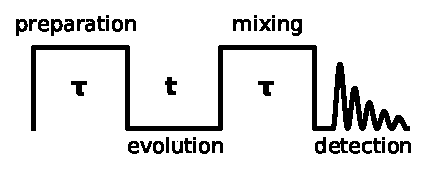
\includegraphics[width=0.5\textwidth]{mq-experiment-schema.pdf}
    %\caption{Схема МК эксперимента ЯМР}
  \end{figure}
  \vspace{-3mm}
  \begin{block}{}
    На подготовительном периоде МК эксперимента ЯМР система облучается последовательностью радиочастотных импульсов. В результате динамика спиновой системы определяется многоквантовым гамильтонианом.
    $$
    H_{MQ} = H^{(2)} + H^{(-2)},
    \quad H^{(\pm2)} = \frac 1 2 \sum_{i < j} D_{ij} I^\pm_i I^\pm_j
    $$
  \end{block}
\end{frame}
\note{
     МК динамику мы решили исследовать стандартным МК экспериментом.
     Эксперимент состоит из четырех частей,
     но нас будет интересовать только подготовительный период эксперимента.
     На подготовительном периоде ...слайд...
}

\begin{frame}{Многоквантовый экперимент ЯМР}
  \begin{columns}
    \column{0.4\textwidth}

    \begin{figure}
      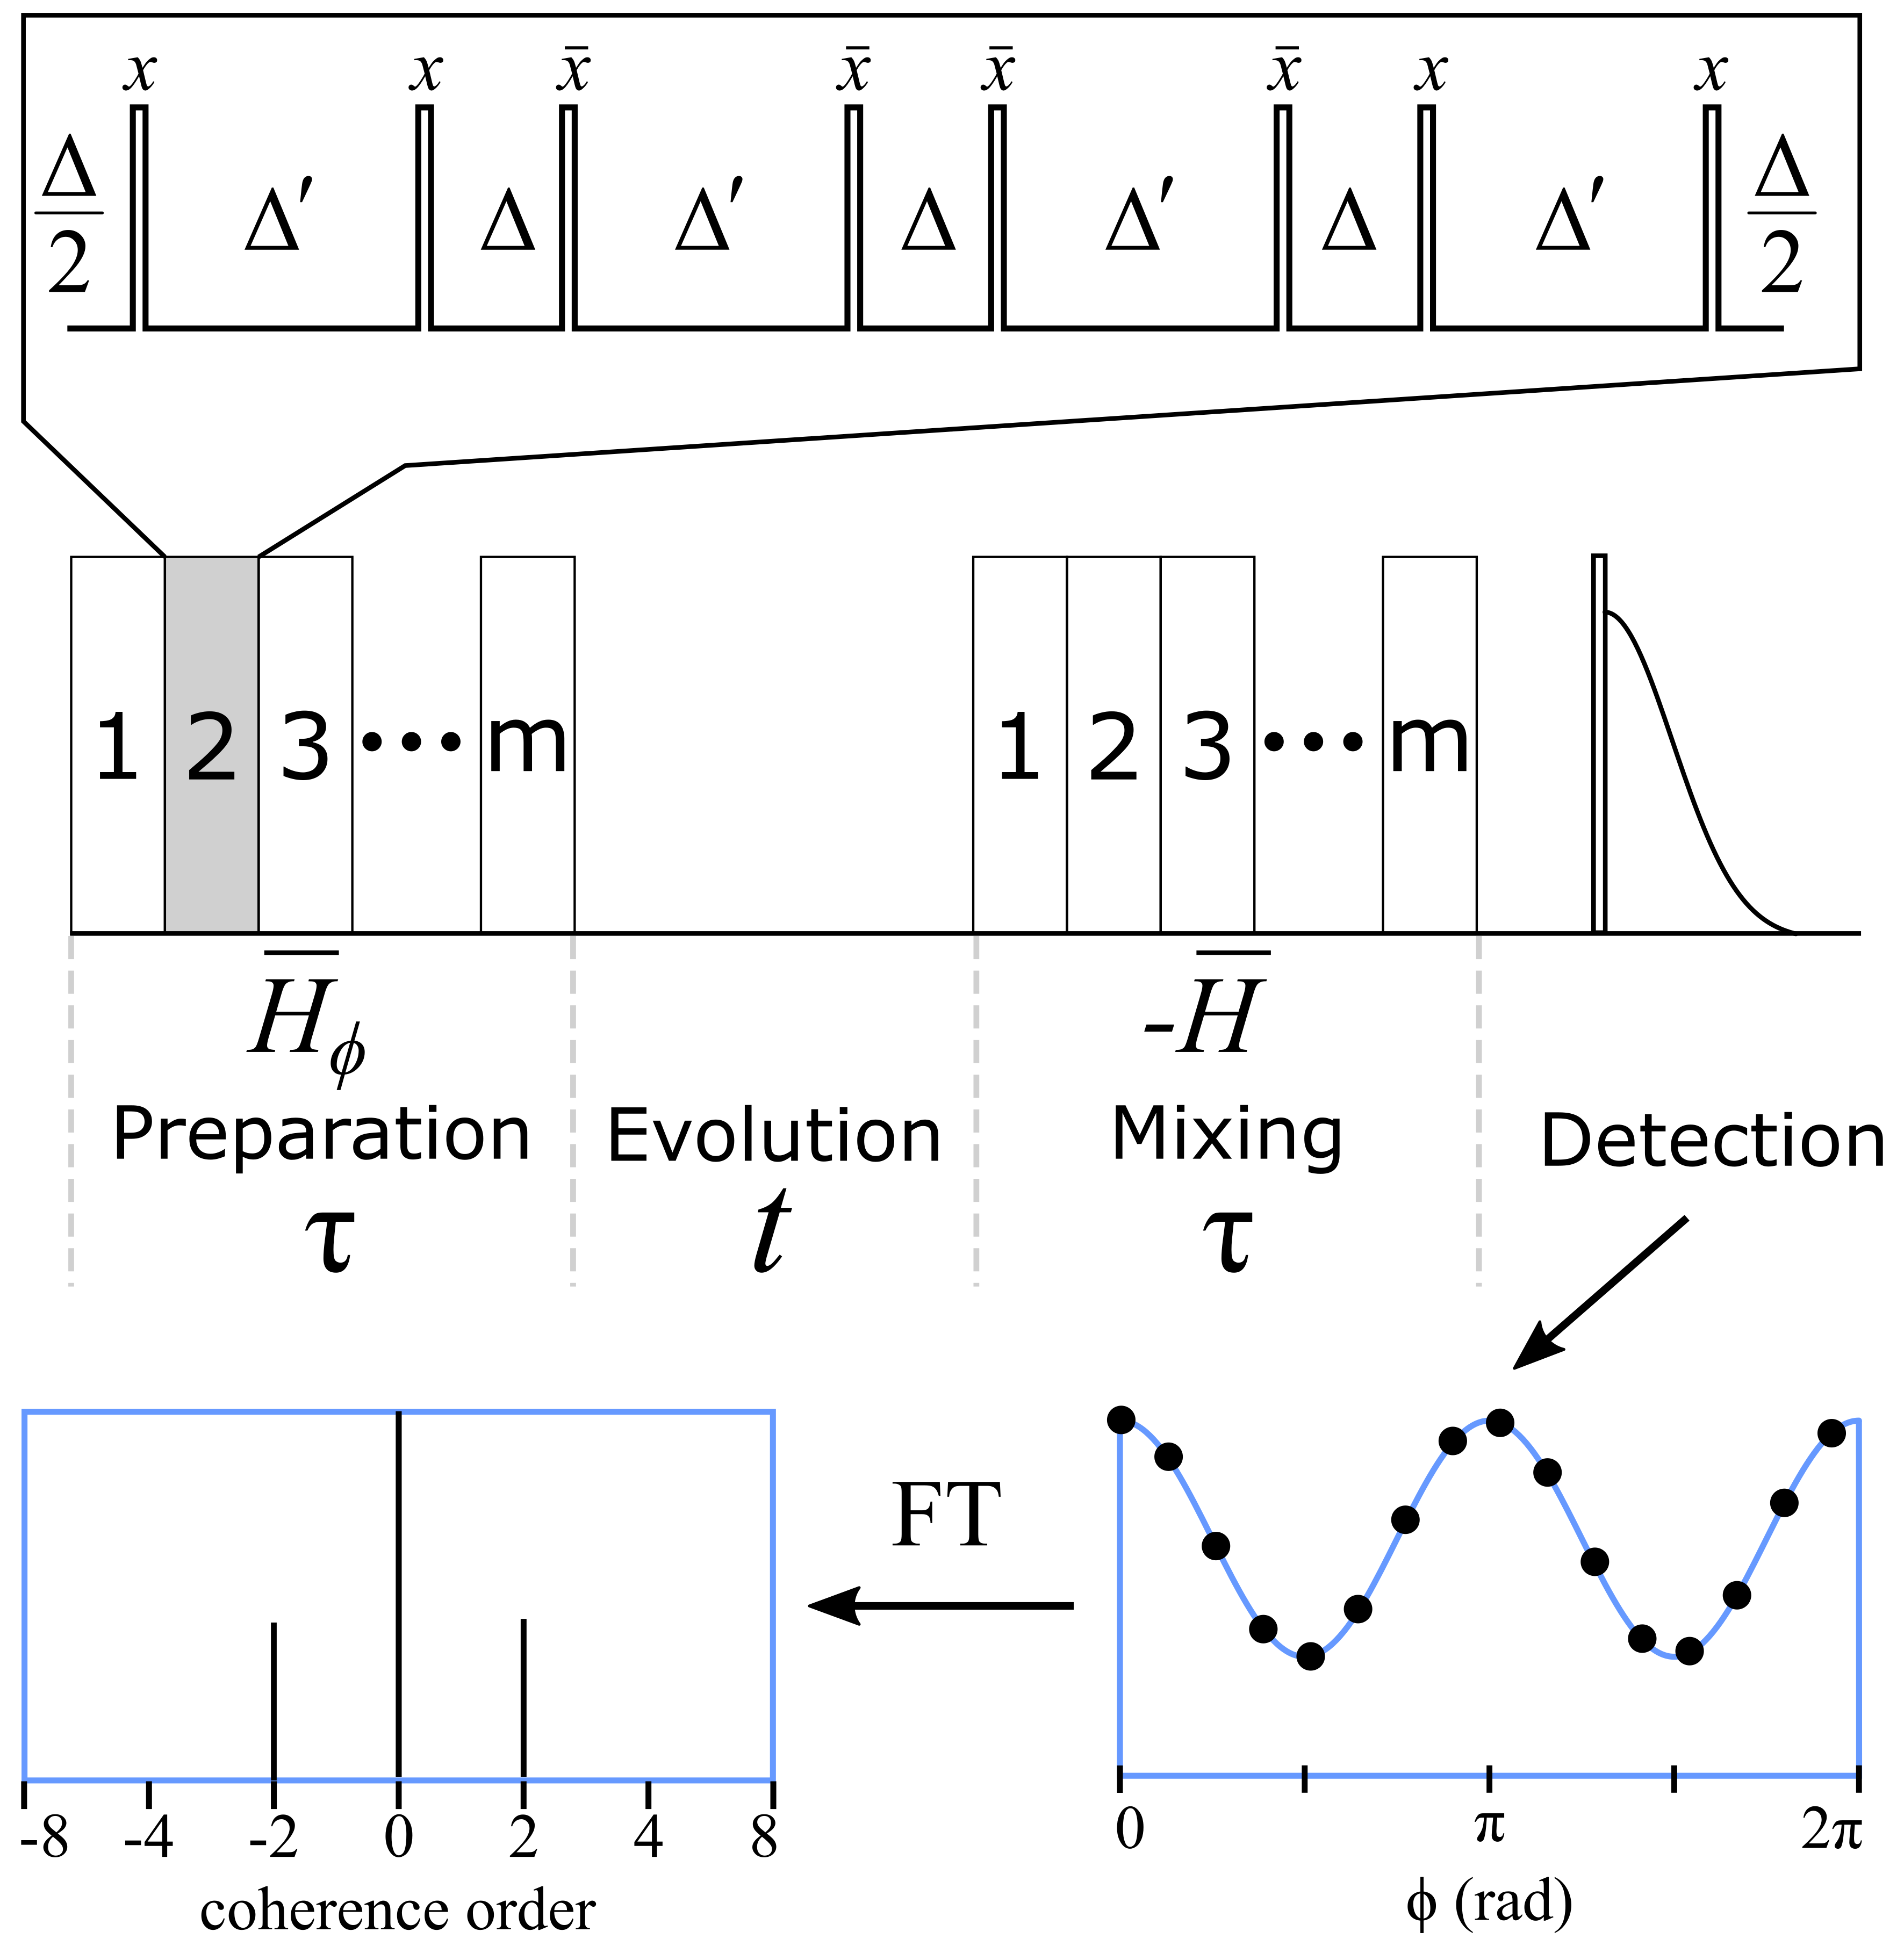
\includegraphics[width=0.9\textwidth]{mq-experiment-pulses-schema.png}
      \caption{Схематичное представление последовательности импульсов МК эксперимента.}
    \end{figure}


    \column{0.6\textwidth}
    МК когерентности создаются в течение периода подготовки продолжительностью $\tau$ при участии m-серии 8-импульсовых подпоследовательностей и затем преобразуются в наблюдаемую намагниченность после идентичного периода смешивания (за исключением 90-градусного фазового сдвига). Затем намагниченность детектируется при импульсе $\pi/2$. Фазовый сдвиг $\phi$ между периодами подготовки и смешивания инкриминируется для разделения многоквантовых когерентностей разных порядков. В результате преобразования Фурье по $\phi$ получается МК ЯМР спектр.
    % Интенсивности МК когерентностей ЯМР при различных длительностях периода свободной эволюции $t$ получаются в отдельных экспериментах.
  \end{columns}
\end{frame}

\begin{frame}{Распределение интенсивности МК когерентностей ЯМР}
\vspace{-5mm}
$$ 
G(\tau, \phi) =
\mathrm{Tr}\left\{
   e^{iH_\mathrm{MQ}\tau} e^{i\phi I_z} e^{-iH_\mathrm{MQ}\tau}
   \rho_\mathrm{eq}
   e^{iH_\mathrm{MQ}\tau} e^{-i\phi I_z} e^{-iH_\mathrm{MQ}\tau}
   I_z 
\right\}
$$
\vspace{-5mm}
\begin{columns}
  \column{0.4\textwidth}
  \vspace{-3mm}
  \begin{figure}
    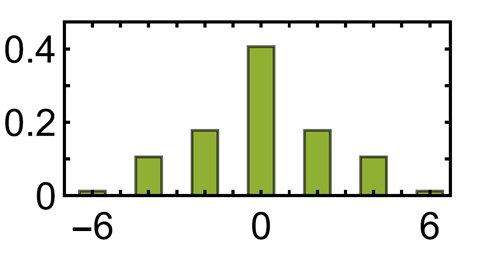
\includegraphics[width=\textwidth]{mq-coherence-intensities-hist.png}
    \caption{$J_{k}$, распределение интенсивности МК когерентностей ЯМР.}
  \end{figure}

  \column{0.5\textwidth}
  \begin{block}{}
    Второй момент (дисперсия) распределения МК когерентностей ЯМР
    $$ M_2 (\tau, \beta) = \sum_n n^2 J_n(\tau, \beta), $$
    где $J_n$ --- интенсивность МК когерентности ЯМР порядка $n$.
  \end{block}
  \begin{alertblock}{}
    %Дисперсия распределения интенсивности МК когерентностей ЯМР определяет нижнюю границу информации
    Квантовая информация Фишера\footnote[frame]{M. G\"arttner, P. Hauke, and A.M. Rey. \textit{Phys. Rev. Lett.} \textbf{120}, 040402 (2018)}
    $$ I_F \geq 2M_2 $$
  \end{alertblock}
\end{columns}
\end{frame}
\note{
  В результате эксперимента получается спектр МК когерентностей для каждого момента времени. 
  Спектр можно охарактеризовать вторым моментом, 
  который вычисляется по формуле. 

  Главным образом второй момент интересен тем, что он связан с нижней границей информации Фишера. 
  Таким образом квантовую информационную величину удается связать с реальной физической наблюдаемой.
  Это открывает возможность экспериментальных исследований связанных с квантовой информации Фишера, 
  в частности исследование многочастичной запутанности в МК эксперименте ЯМР. 
  % ЯМР отличный инструмент и наша работа это подтверждает.
  % mq-coherences-distribution % JETP 2018
}



\section{Измерение информации Фишера в МК эксперименте ЯМР}
% \chapter{Измерение квантовой информации Фишера в МК эксперименте ЯМР}
\chapter{Измерение информации Фишера в МК эксперименте ЯМР}
\label{chapter:quantum-fisher-information-measurement}
% (PRA-2019)
% - Расчет динамики при низкой температуре
% - Вычисление второго момента

В разделе~\ref{sec:quantum-fisher-information-mesuarement-at-high-temperature}
была обсуждена связь между вторым моментом распределения интенсивностей МК когерентностей ЯМР и квантовой информацией Фишера~\cite{Toth2014,Pezze2018}.
В частности, было показано,
что в классическом эксперименте ЯМР, когда сигнал усредняется по наблюдаемой $I_z$, в области высоких температур второй момент МК спектра соответствует нижней границе квантовой информации Фишера~\cite{Garttner2018}.
Ниже будет показано, что МК эксперимент ЯМР может быть проведен таким образом,
что связь квантовой информации Фишера и второго момента сохранится для произвольных температур.


\section{МК динамика ЯМР при низких температурах}
%\section{МК когерентности ЯМР}
\begin{figure}[H]
  \centering
  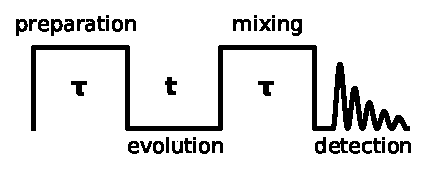
\includegraphics[width=0.5\textwidth]{mq-experiment-schema.pdf}
  \caption{Схема МК эксперимента ЯМР}
  \label{fig:mq-experiment-schema}
\end{figure}

Первоочередно рассмотрим теорию МК динамики ЯМР (см. раздел~\ref{sec:mq-nrm-experiment})
для термодинамически равновесного начального состояния системы $\rho_\mathrm{eq}$,
которое определяется выражением
%
\begin{equation}
  \label{eq:rho_eq}
  \rho_{\mathrm{eq}} = \dfrac{e^{\frac{\hbar\omega_{0}}{kT} I_z}}{Z},
\end{equation}
%
где $Z =\mathrm{Tr}\left\{e^{\frac{\hbar\omega_{0}}{kT} I_z}\right\}$ это статистическая сумма,
$\hbar$ и $k$ --- это постоянная Планка и постоянная Больцмана,
$\omega_0$ --- Ларморовская частота,
$T$ --- температура,
и $I_z$ это оператор проекции полного углового момента на ось $z$,
которая направлена вдоль сильного внешнего магнитного поля.

Для теоретического исследования МК динамики ЯМР
необходимо найти эволюционную матрицу плотности $\rho(\tau)$
на подготовительном периоде МК эксперимента ЯМР (см. раздел~\ref{sec:mq-nrm-experiment}),
решив уравнение Лиувилля~\cite{Feldman2012}
%
\begin{equation}
    \label{eq:liouvile}
    i \dfrac{d\rho(\tau)}{d \tau} =
    \left[H_\mathrm{MQ}, \rho(\tau)\right].
\end{equation}
%
с начальной матрицей плотности $\rho(0)$,
находящейся в термодинамическом равновесии,
%
\begin{equation}
    \label{eq:rho_init}
    \rho(0) = \rho_{\mathrm{eq}}.
\end{equation}
%
Так как в рассматриваемом случае гамильтониан~$H_\mathrm{MQ}$
не зависит от времени,
эволюционная матрица плотности может быть выражена как
\begin{equation}
  \label{eq:rho_eval_lt}
  \rho_\mathrm{LT} (\tau) = e^{-iH_\mathrm{MQ}\tau} \rho_\mathrm{eq} e^{iH_\mathrm{MQ}\tau},
\end{equation}
В области высоких температур,
когда $b = \frac{\hbar\omega_{0}}{kT} \ll 1$,
начальную матрицу плотности $\rho_{\mathrm{eq}}$ можно разложить в ряд по $b$:
%
\begin{equation}
  \label{eq:rho_ht}
  \rho_{\mathrm{eq}} \approx \dfrac{1}{2^N} (1 + bI_z).
\end{equation}
%
В этом случае эволюционную матрицу плотности можно переписать, как
\begin{equation}\label{eq:rho_eval_ht}
  \rho_\mathrm{HT} (\tau) =  e^{-iH_\mathrm{MQ}\tau} I_z e^{iH_\mathrm{MQ}\tau},
\end{equation}

Экспериментальное исследование МК динамики ЯМР заключается в проведении
МК эксперимента ЯМР (см. раздел~\ref{sec:mq-nrm-experiment})
и последующем измерении интенсивностей МК когерентностей ЯМР.
В результате проведения всех периодов МК эксперимента ЯМР (Рис.~\ref{fig:mq-experiment-schema})
итоговый сигнал $G(\tau, \phi)$ хранится в информации о населенности\cite{Feldman1997}.
Выражение для сигнала $G(\tau, \phi)$ имеет вид
%
\begin{equation}
  \label{eq:signal}
   G(\tau, \phi)
   = \tr{
     e^{iH_\mathrm{MQ}\tau} e^{i\phi I_z} e^{-iH_\mathrm{MQ}\tau}
     \rho_\mathrm{eq}
     e^{iH_\mathrm{MQ}\tau} e^{-i\phi I_z} e^{-iH_\mathrm{MQ}\tau}
     I_z
    }.
\end{equation}
%
Перегруппировкой множителей,
выражение~(\ref{eq:signal}) может быть переписано через
 $\rho_\mathrm{LT} (\tau)$ и $\rho_\mathrm{HT} (\tau)$:
%
\begin{equation}
  \label{eq:signal-short}
  G(\tau, \phi) = \tr{
   e^{i\phi I_z} \rho_\mathrm{LT} (\tau)
   e^{-i\phi I_z} \rho_\mathrm{HT} (\tau).
  }
\end{equation}


Для получения выражений сигналов отдельных когерентностей,
перейдем к представлению матриц плотности
$\rho_\mathrm{LT} (\tau)$ и $\rho_\mathrm{HT} (\tau)$
в виде ряда
%
\begin{equation}\label{eq:rho_series}
  \rho_\mathrm{LT} (\tau) = \sum_n \rho_{LT, n}(\tau); \quad
  \rho_\mathrm{HT} (\tau) = \sum_n \rho_{HT, n}(\tau),
\end{equation}
%
где $\rho_{LT, n} (\tau)$ и  $\rho_{HT, n} (\tau)$
это вклад МК когерентности $n$-ого порядка
в матрицы плотности $\rho_\mathrm{LT} (\tau)$ и $\rho_\mathrm{HT} (\tau)$ соответственно.
Подставляя~(\ref{eq:rho_series}) в~(\ref{eq:signal}) итоговый сигнал $G(\tau, \phi)$ МК когерентностей ЯМР можно переписать как
%
\begin{equation}
    \label{eq:signal_series}
    G(\tau, \phi) = \sum\limits_n
    e^{in\phi}\mathrm{Tr} \left\{
    \rho_{LT, n}(\tau) \rho_{HT, -n} (\tau)
    \right\},
\end{equation}
%
где учтены коммутационные соотношения
%
\begin{equation}
    \left[I_z, \rho_{LT, n} (\tau) \right] = n  \rho_{LT, n} (\tau);
    \quad
    \left[I_z, \rho_{HT, n} (\tau) \right] = n  \rho_{HT, n} (\tau).
\end{equation}

Нормированные интенсивности МК когерентностей ЯМР могут быть выражены следующим образом
%
\begin{equation}
    \label{eq:coherence}
    J_n(\tau)
    = \dfrac{
       \mathrm{Tr} \left\{
        \rho_{LT, n}(\tau) \rho_{HT, -n} (\tau)
        \right\}
    }{Tr \left\{\rho_{\mathrm{eq}}I_z\right\}}.
    = \dfrac{
       \mathrm{Tr} \left\{
        \rho_{LT, n}(\tau) \rho_{HT, -n} (\tau)
        \right\}
    }{\frac N 2 \tanh \frac b 2}.
\end{equation}

МК когерентности ЯМР имеют несколько свойств.
Во-первых, в момент времени  $\tau=0$
нормированная интенсивность $J_0(0)$ МК когерентности ЯМР нулевого порядка равна 1,
а остальные интенсивности равны нулю.
Во-вторых, сумма всех нормированных когерентностей равна единице.
Докажем это утверждение.
Используя выражения~(\ref{eq:rho_eq}) и~(\ref{eq:rho_eval_ht})
выразим $\rho_\mathrm{LT}(\tau)$ через $\rho_\mathrm{HT}(\tau)$.
%
\begin{equation}\label{eq:lt-through-ht}
  \rho_\mathrm{LT}(\tau) = \dfrac 1 Z
  \exp\left(be^{-iH_\mathrm{MQ}\tau} I_z e^{iH_\mathrm{MQ}\tau}\right) =
  \dfrac 1 Z e^{b\rho_\mathrm{HT}(\tau)}.
\end{equation}
%
Подставляя выражение~(\ref{eq:lt-through-ht}) в~(\ref{eq:coherence}) получаем
%
\begin{multline}
  \label{eq:sum_of_coherence}
  \sum\limits_n J_n(\tau) =
  \dfrac{\sum\limits_{n, m}\mathrm{Tr}\left\{
      \rho_{LT, n}(\tau)\rho_{HT, m}(\tau)
  \right\}}
  {\mathrm{Tr}\left\{\rho_\mathrm{eq} I_z\right\}} = \\
  \dfrac{\mathrm{Tr}\left\{
      \rho_\mathrm{LT}(\tau)\rho_\mathrm{HT}(\tau)
  \right\}}
  {\mathrm{Tr}\left\{\rho_\mathrm{eq} I_z\right\}} =
  \dfrac{\mathrm{Tr}\left\{
      \rho_\mathrm{HT}(\tau)e^{b\rho_\mathrm{HT}(\tau)}
  \right\}}
  {Z\mathrm{Tr}\left\{\rho_\mathrm{eq} I_z\right\}} = \\
  \dfrac{\frac{d}{db} \ln \mathrm{Tr}\left\{
      e^{b I_z}
  \right\}}
  {\mathrm{Tr}\left\{\rho_\mathrm{eq} I_z\right\}} =
  \dfrac{\frac 1 2 N \tanh \left( \frac b 2 \right)}
  {\frac 1 2 N \tanh \left( \frac b 2 \right)} = 1.
\end{multline}
Ур.~(\ref{eq:sum_of_coherence}) подтверждает,
что сумма МК когерентностей ЯМР сохраняется на подготовительном периоде МК эксперимента ЯМР.


\section{Приведенные МК когерентности ЯМР}
\label{sec:reduced-mq-coherences}

В предыдущем разделе было получено выражение~(\ref{eq:signal-short}) коррелятора сигнала $G(\tau, \phi)$,
которое в области высоких температур имеет вид
%
\begin{equation}
    \label{eq:otoc-ht}
    G_\mathrm{HT}(\tau, \phi) = \frac b Z\mathrm{Tr}\left\{
    e^{i \phi I_z}
    \rho_\mathrm{HT} (\tau)
    e^{-i \phi I_z}
    \rho_\mathrm{HT}(\tau)
    \right\},
\end{equation}
%
так как согласно разложению~(\ref{eq:rho_ht})
%
\begin{equation}
  \rho_\mathrm{LT} (\tau) \approx \frac 1 Z + \frac b Z \rho_\mathrm{HT}.
\end{equation}
%
Так же в разделе~\ref{sec:quantum-fisher-information-mesuarement-at-high-temperature}
было отмечено,
что связь второго момента МК спектра ЯМР и квантовой информации Фишера
обеспечивается благодаря особому виду коррелятора сигнала.
% Коррелятор должен принадлежать классу неупорядоченных по времени корреляторов ``out-of-time-ordered correlator'' (OTOC).
Выражение~(\ref{eq:otoc-ht}) для $G_\mathrm{HT}(\tau, \phi)$
в высоко температурной области
удовлетворяет этому требованию,
в отличие от выражения~(\ref{eq:signal-short}) для $G(\tau, \phi)$.
$G(\tau, \phi)$ не является неупорядоченным по времени коррелятором,
так как выражение~(\ref{eq:signal}) содержит разные матрицы $\rho_\mathrm{LT}(\tau)$ и $\rho_\mathrm{HT}(\tau)$.
Однако можно обобщить МК эксперимент ЯМР  таким образом,
чтобы привести сигнал $G(\tau, \phi)$ к нужному виду.
Для достижения такого поведения коррелятора финального сигнала МК эксперимента ЯМР
необходимо усреднить сигнал,
полученный после трех периодов %МК эксперимента ЯМР
(Рис.~\ref{fig:mq-experiment-schema}),
по начальному состоянию $\rho_\mathrm{eq}$.
Тогда коррелятор сигнала будет описываться следующим выражением
%
\begin{multline}
  \label{eq:otoc_LT}
  G_\mathrm{LT}(\tau, \phi) =
  \mathrm{Tr}\left\{
    e^{i H_{\mathrm{MQ}} \tau}
    e^{i \phi I_z}
    e^{-i H_{\mathrm{MQ}} \tau}
    \rho_{\mathrm{eq}}
    e^{i H_{\mathrm{MQ}}}
    e^{-i \phi I_z}
    e^{-i H_{\mathrm{MQ}} \tau}
    \rho_{\mathrm{eq}}
  \right\} \\ =
  \mathrm{Tr}\left\{
    e^{i \phi I_z}
    e^{-i H_\mathrm{MQ} \tau}
    \rho_\mathrm{eq}
    e^{i H_\mathrm{MQ} \tau}
    e^{-i \phi I_z}
    e^{-i H_\mathrm{MQ} \tau}
    \rho_{\mathrm{eq}}
    e^{i H_\mathrm{MQ} \tau}
  \right\} \\ =
  \mathrm{Tr}\left\{
    e^{i \phi I_z}
    \rho_\mathrm{LT} (\tau)
    e^{-i \phi I_z}
    \rho_\mathrm{LT} (\tau)
  \right\}.
\end{multline}
%
Из выражения~(\ref{eq:otoc_LT}) следует,
что $G_\mathrm{LT}(\tau, \phi)$ является неупорядоченным по времени коррелятором при произвольных температурах.
Важно отметить,
что полученный результат для начальной матрицы~(\ref{eq:rho_eq}) легко обобщить
на произвольное начальное состояние.
Связь квантовой информации Фишера и второго момента будет выполняться всегда,
если по итогу трех периодов (Рис.~\ref{fig:mq-experiment-schema}) МК экскремента ЯМР
проводить усреднение по начальному состоянию.
Это наблюдение будет играть важную роль в следующей Главе~\ref{chapter:manyparticle-entanglement-in-nanopore}
при рассмотрении МК динамики ЯМР дипольных упорядоченных состояний.

Нормированные интенсивности МК когерентностей ЯМР для сигнала $G_\mathrm{LT}(\tau, \phi)$
могут быть записаны по аналогии с~(\ref{eq:coherence}):
%
\begin{equation}\label{eq:reduced-mq-coherences}
    J_{\mathrm{LT}, n}(\tau) =
    \frac{\mathrm{Tr} \left\{
        \rho_{\mathrm{LT},n}(\tau)
        \rho_{\mathrm{LT}, -n}(\tau)
    \right\}}
    {\mathrm{Tr}\left\{\rho^2_\mathrm{eq}\right\}}.
\end{equation}
%
В этом случае нормировочный член определяется как
%
\begin{equation}\label{eq:j_lt_norm}
  \mathrm{Tr}\left\{\rho^2_\mathrm{eq}\right\} =
    \frac{2^N \cosh^N(b)}{Z^2}.
\end{equation}
Когерентности определяемые выражением~(\ref{eq:reduced-mq-coherences})
являются приведенными МК когерентностями ЯМР.
%
Используя разложение~(\ref{eq:rho_series}),
сумма интенсивностей приведенных МК когерентностей ЯМР~(\ref{eq:reduced-mq-coherences}) может быть записана как
%
\begin{multline}\label{eq:reduced-coherences-sum}
  \sum\limits_{n} J_{\mathrm{LT}, n}(\tau)
  = \dfrac{
    \tr{
      \sum\limits_{n}
      \rho_{\mathrm{LT}, n}(\tau)
      \rho_{\mathrm{LT},-n}(\tau)}
    }{
    \tr{\rho^2_\mathrm{eq} }
  }
  = \dfrac{
    \tr{
      \sum\limits_{m,n}
      \rho_{\mathrm{LT}, n}(\tau)
      \rho_{\mathrm{LT}, m}(\tau)
    }}{
    \tr{\rho^2_\mathrm{eq}}
  }
  \\
  = \dfrac{
    \tr{\rho_\mathrm{LT}^2(\tau)}
  }{
    \tr{\rho^2_\mathrm{eq}(\tau)}
  }
  = \dfrac{
    \tr{
      e^{-i H_\mathrm{MQ} \tau}
      \rho^{2}_\mathrm{eq}
      e^{i H_\mathrm{MQ} \tau}
    }
  }{
    \tr{ \rho^2_\mathrm{eq}}
  }
  = 1.
\end{multline}
%
Из уравнения~(\ref{eq:reduced-coherences-sum}) можно сделать вывод, что сумма МК~когерентностей~ЯМР~сохраняется на подготовительном периоде МК~эксперимента~ЯМР~\cite{Baum1985}.


Удвоенный второй момент (дисперсия) $M_2(\tau)$ распределения интенсивностей приведенных МК когерентностей ЯМР $J_{\mathrm{LT}, n} (\tau)$
является нижней границей квантовой информации Фишера $F_{Q}$
(см. раздел~\ref{sec:quantum-fisher-information-mesuarement-at-high-temperature}):
\begin{equation}\label{eq:fisher-low-bound}
  F_{Q}(\tau) \geq 2M_2(\tau),
\end{equation}
где второй момент может быть выражен~\cite{Khitrin1997} как
%
\begin{equation}\label{eq:m2-via-coherences}
  M_2(\tau) = \sum\limits_n n^2 J_{\mathrm{LT}, n} (\tau).
\end{equation}

\section{Выводы}
В этой главе было предложено обобщение МК эксперимента ЯМР,
позволяющее измерять нижнюю границу квантовой информации Фишера
в произвольный момент времени подготовительного периода МК эксперимента ЯМР
с произвольным начальным состоянием системы.
В свою очередь квантовая информация Фишера является ключевой концепцией в квантовой теории информации
и основной мерой в квантовой метрологии.
В частности квантовая информация Фишера может выступать в качестве количественной оценки запутанных частиц в системе.
Таким образом, становится возможным исследование многочастичной запутанности в МК эксперименте ЯМР.
Более того, разработанный подход позволяет исследовать температурную зависимость многочастичной запутанности.

% При высоких температурах интенсивность МК когерентностей ЯМР может быть исследована экспериментально с помощью обычных МК экспериментов ЯМР.
Результаты полуаналитического анализа многочастичной запутанности в системе спин-несущих молекул (атомов) представлены в следующей главе~\ref{chapter:manyparticle-entanglement-in-nanopore}.

\section{Многочастичная запутанность в системе эквивалентных спинов}
\begin{frame}{Система эквивалентных спинов}
  \begin{figure}
    \begin{subfigure}[t]{0.32\textwidth}
      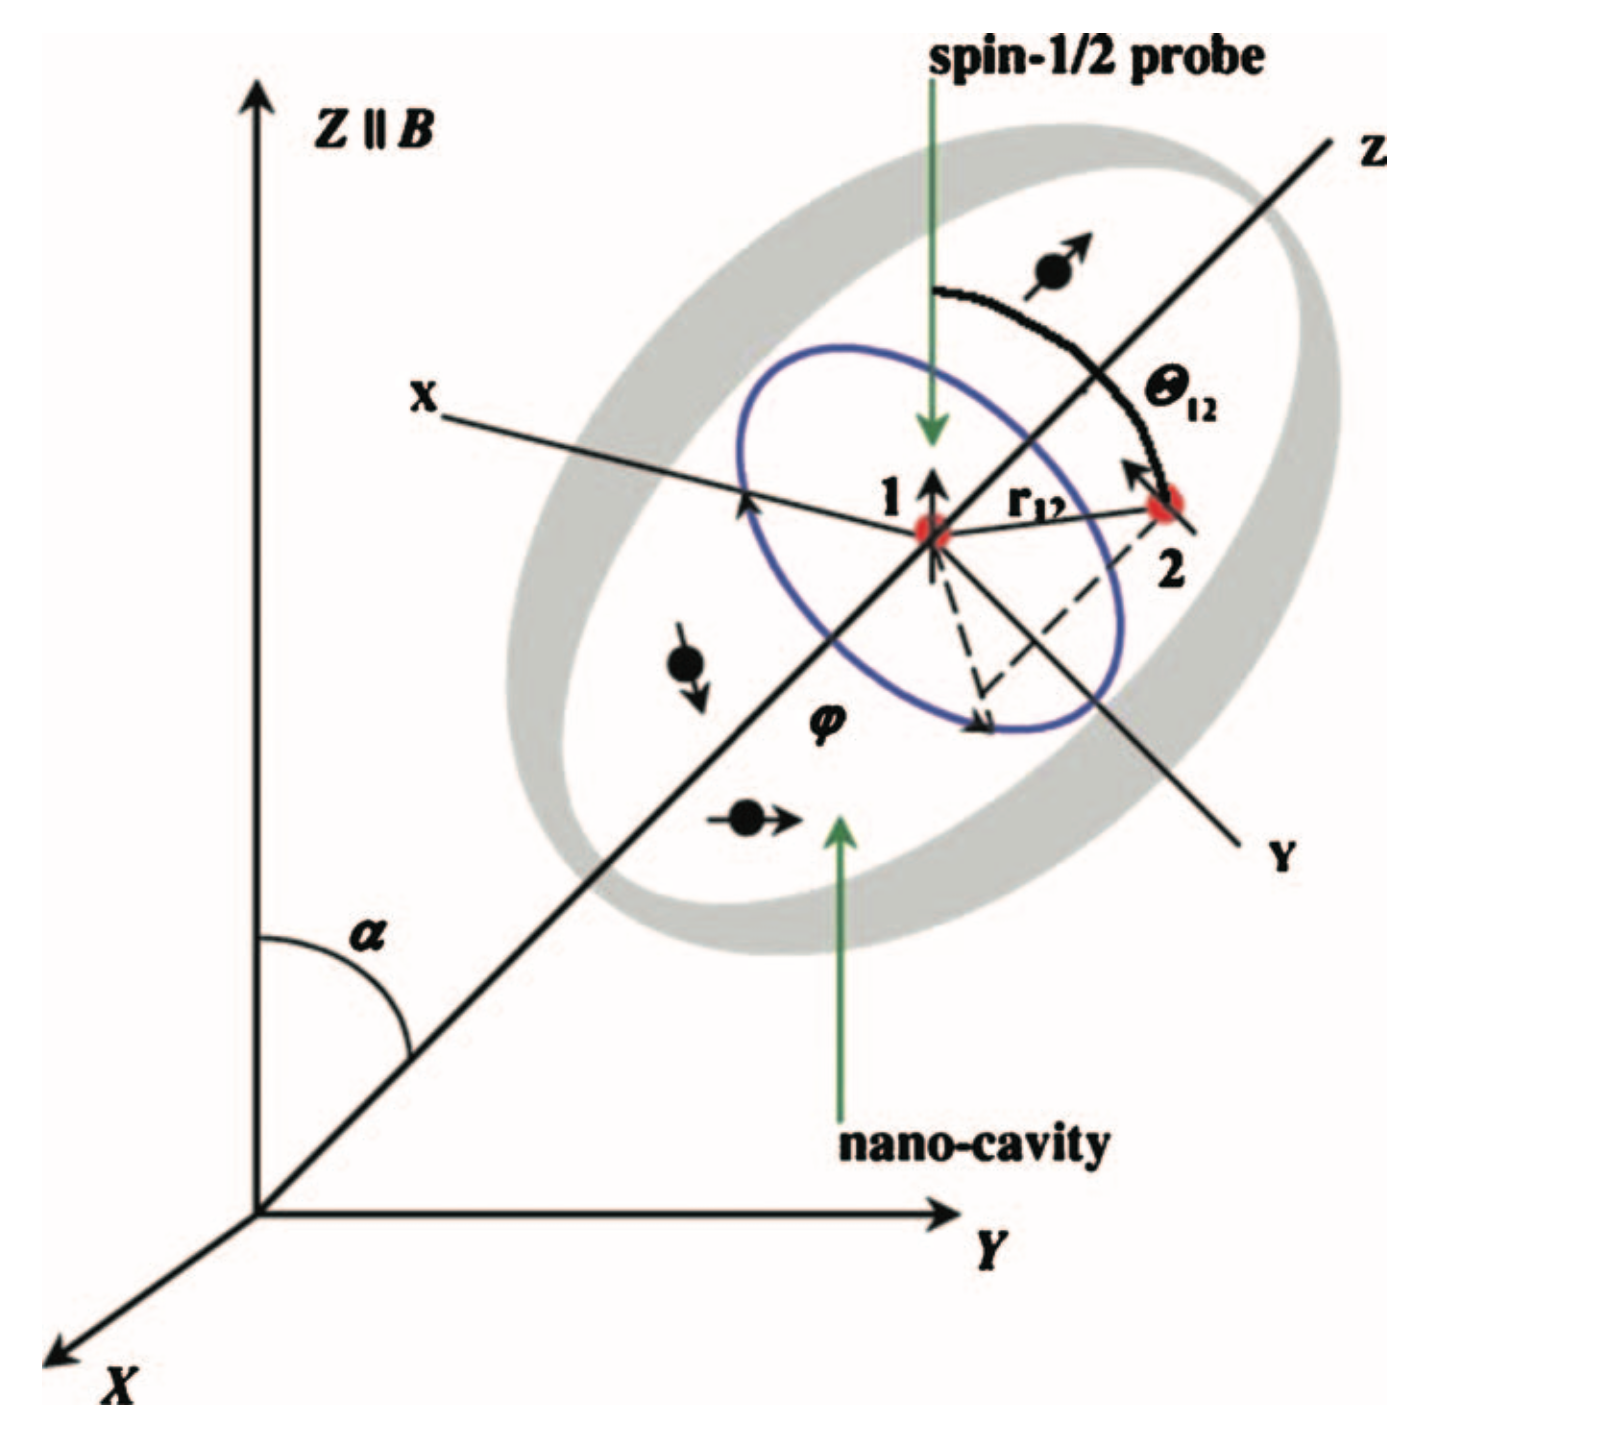
\includegraphics[width=\textwidth]{model-nanopore-schema.png}
      \caption{
        Hанопора,
        заполненная спин-несущими молекулами во внешнем сильном магнитном поле $\vec B$.
      }
    \end{subfigure}
    \hfill
    \begin{subfigure}[t]{0.32\textwidth}
      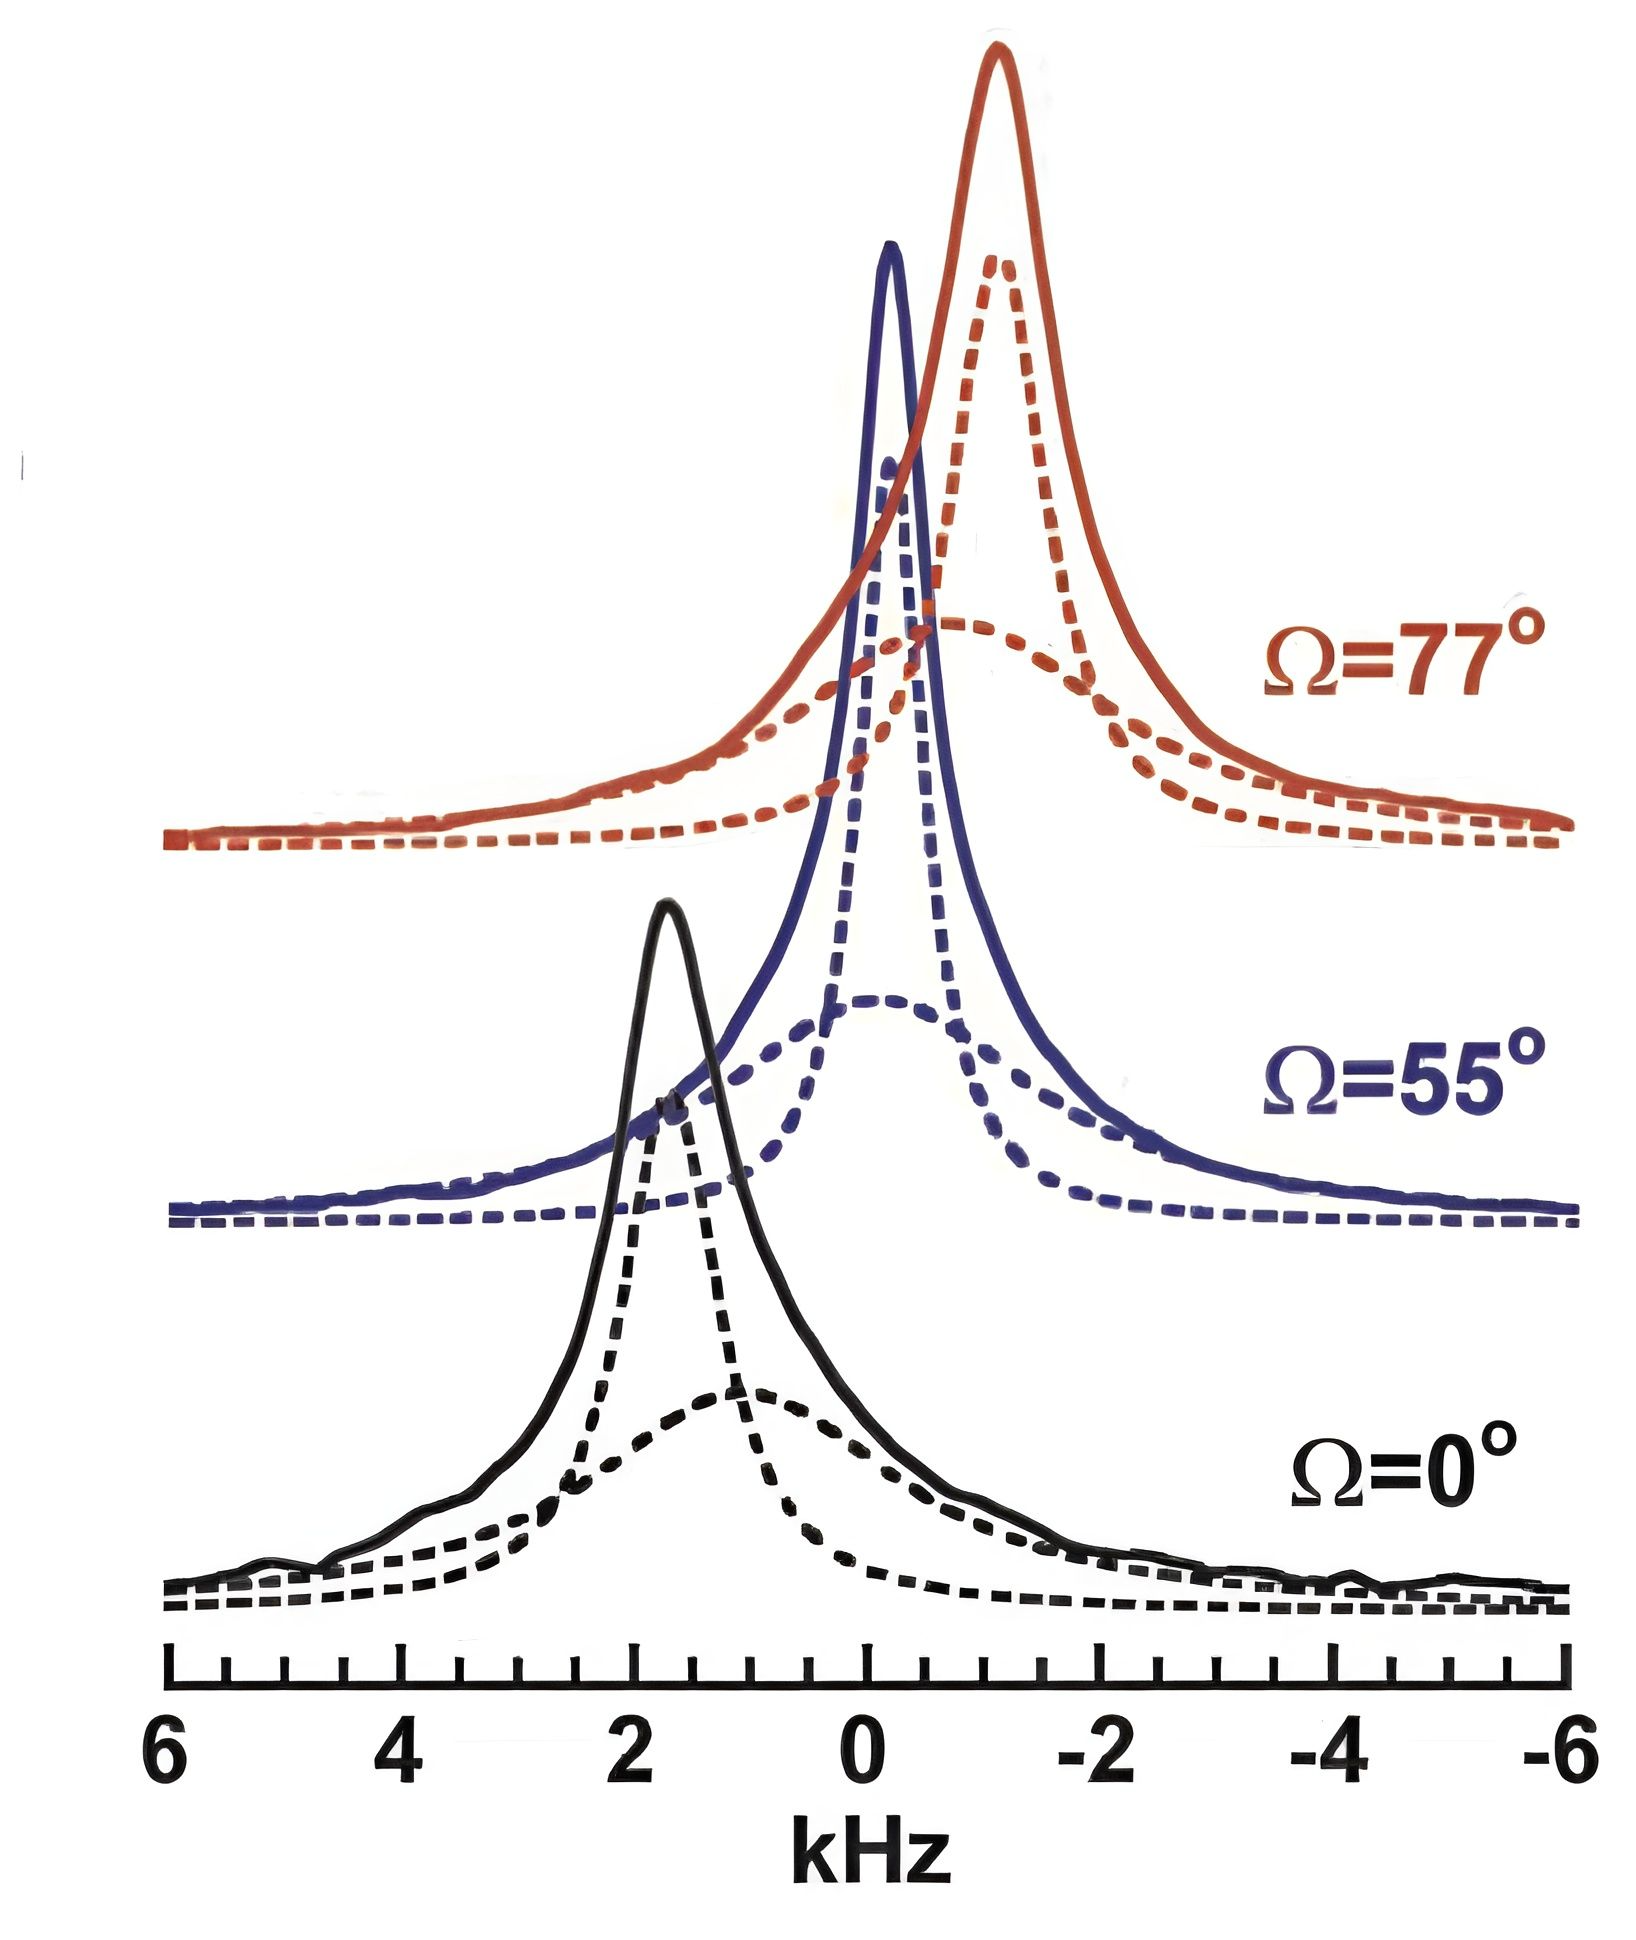
\includegraphics[width=0.8\textwidth]{sample-nanopore-nmr-spectrum.png}
      \caption{
        Молекулярная диффузия газа быстрее флип-флоп процессов.
        Вся система характеризуется одной константой $D$.
      }
    \end{subfigure}
    \hfill
    \begin{subfigure}[t]{0.32\textwidth}
      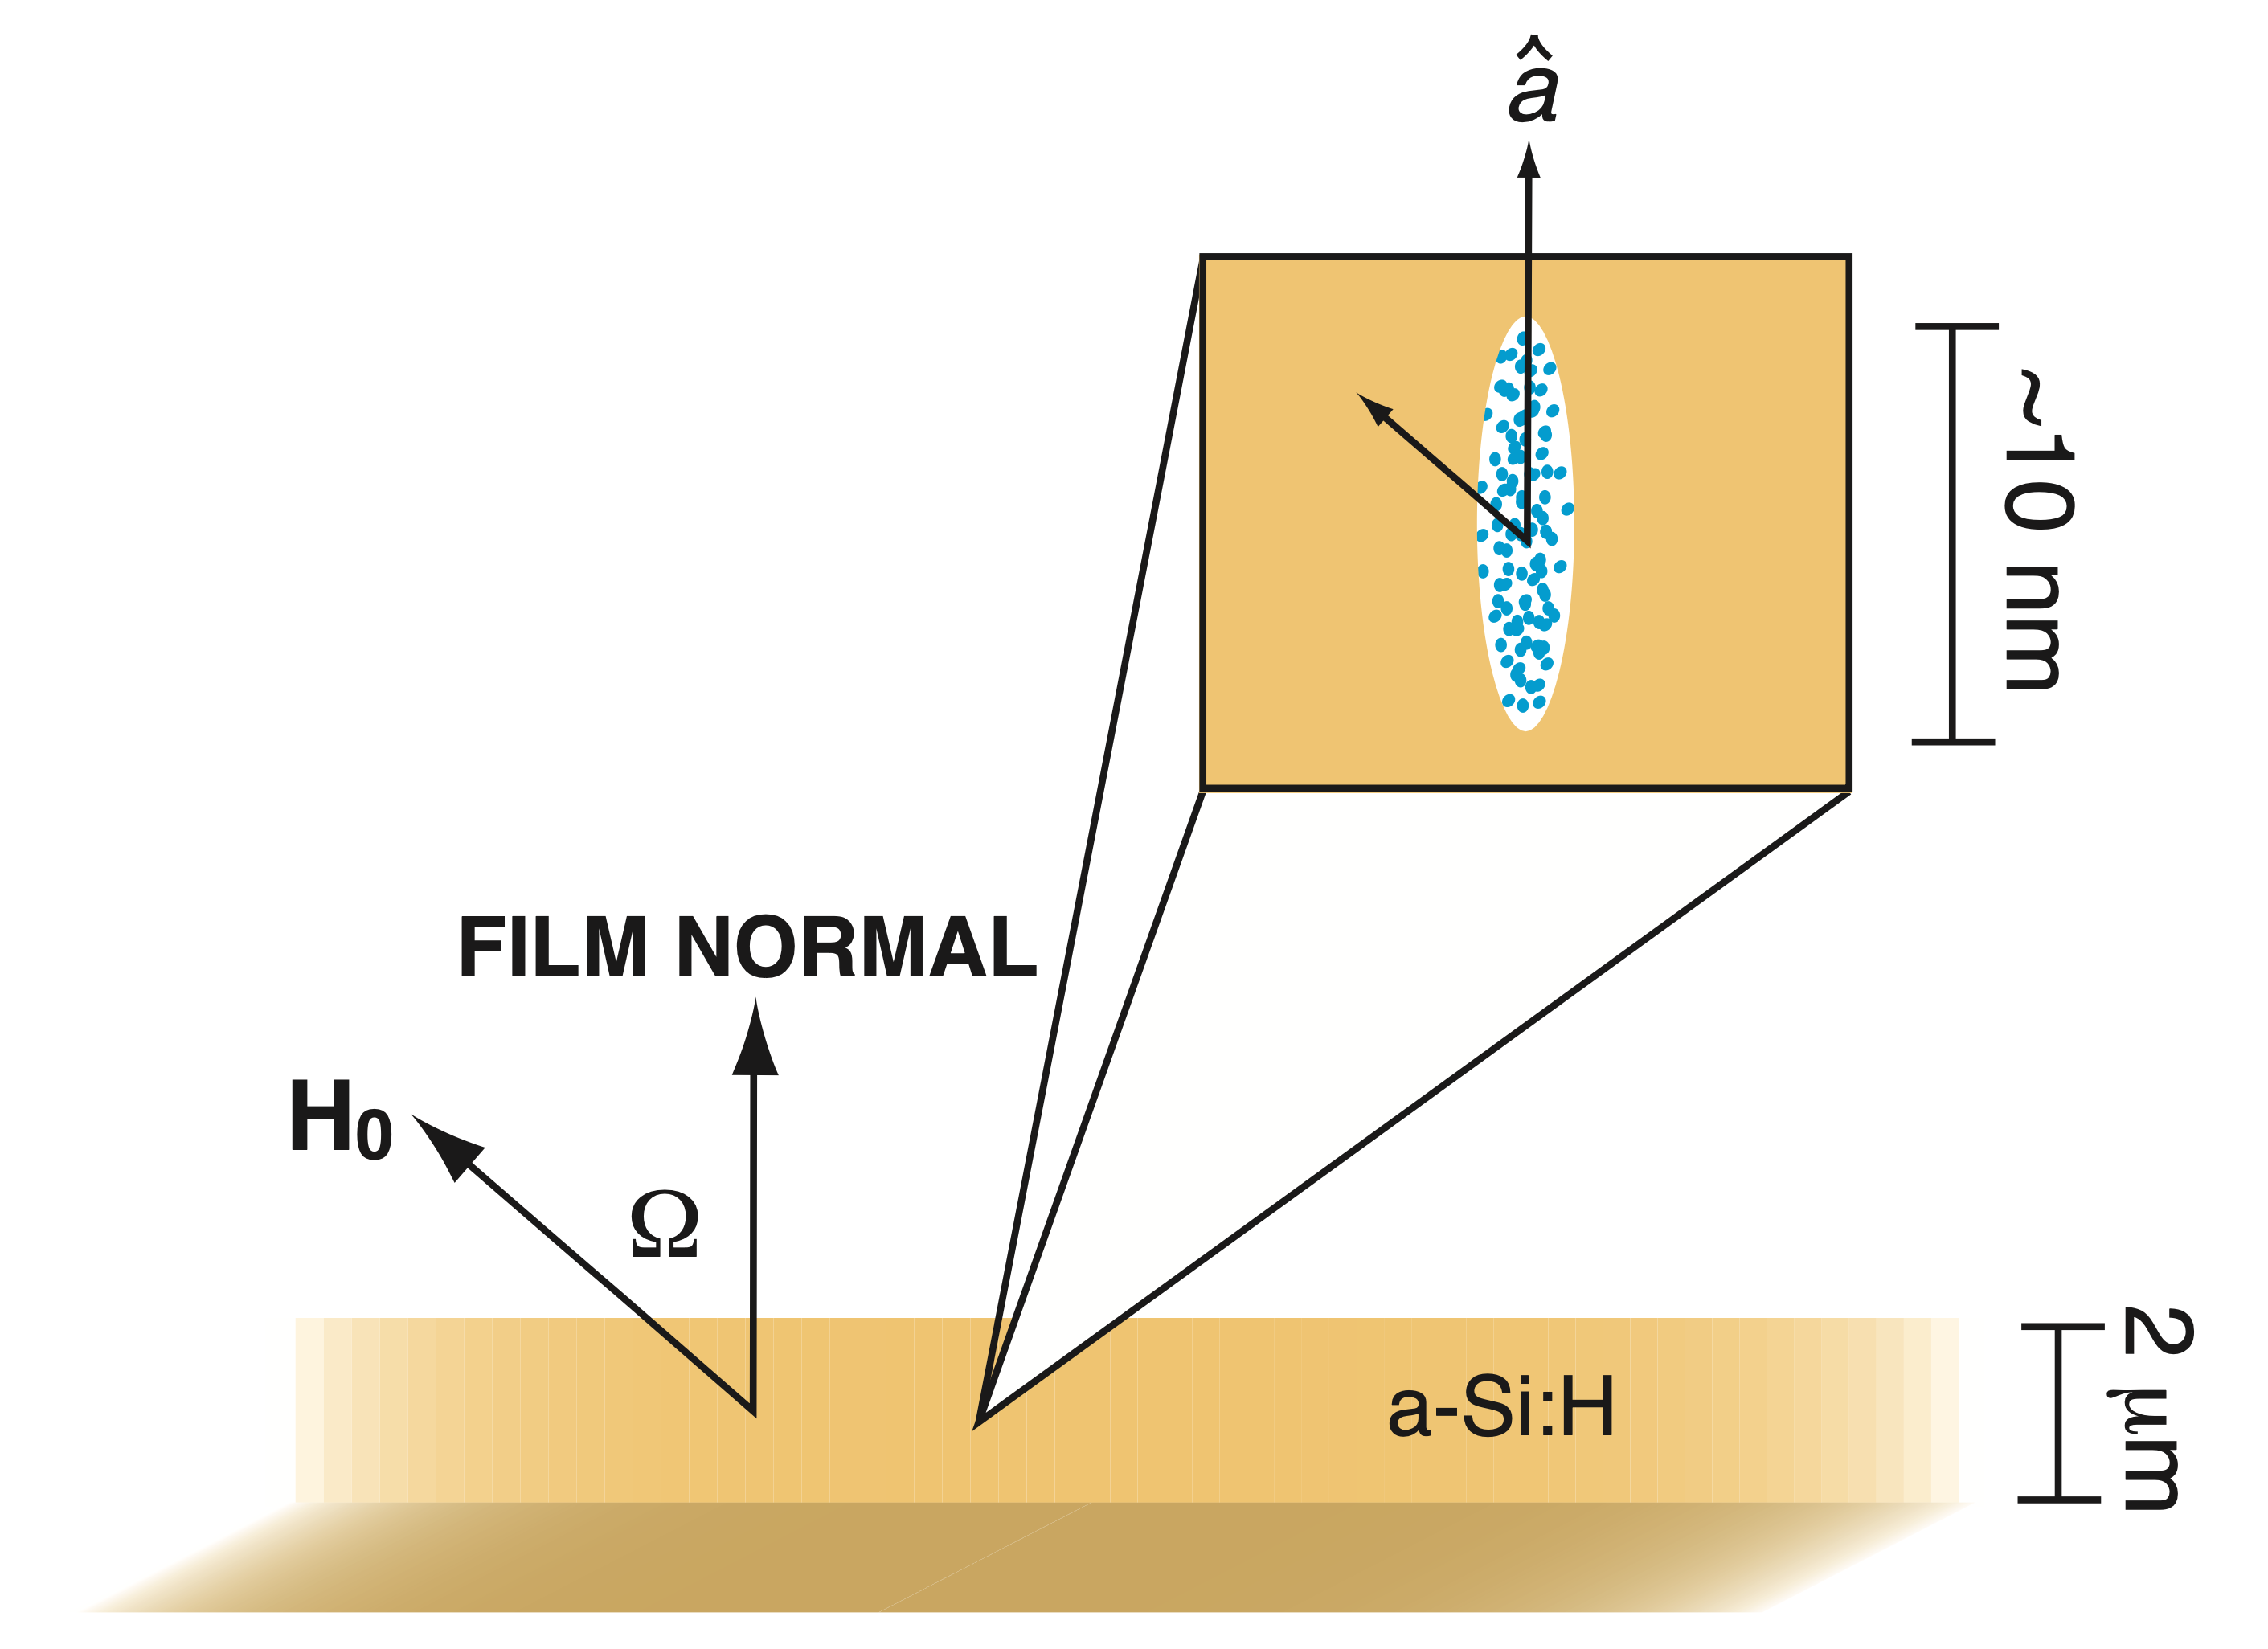
\includegraphics[width=\textwidth]{sample-nanopore-film.png}
      \caption{
        Значение константы связи $D$ зависит как от газа,
        так и от эффективного давления в нанопоре ($\approx 1$ кБар)
      }
    \end{subfigure}
    \captionsetup{skip=-0.1mm}
    \caption{J. Baugh, A. Kleinhammes, D. Han, Q. Wang, and Y. Wu, \textit{Science} \textbf{294}, 1505 (2001).}
  \end{figure}

  % \begin{block}{Нанопора\footnote[frame]{J. Baugh, A. Kleinhammes, D. Han, Q. Wang, and Y. Wu, Science 294, 1505 (2001).}, заполненая частицами со спином $1/2$}
  %     Так как молекулярная диффузия газа быстрее флип-флоп процессов,
  %     вся система характеризуется одной константой взаимодейсвия $D$.
%
  %     \vspace{\baselineskip}
%
  %     Значение константы связи $D$ зависит как от газа, так и от эффективного давления в нанопоре ($\approx 1$ кБар).
  % \end{block}
\end{frame}
\note{
    Hydrogenated amorphous silicon (Гидрогенизированный аморфный кремний)

    Для исследования многочастичной запутанности нам нужна модель,
    в которой почти все частицы взаимодействуют друг с другом.
    % а также она должна поддаваться счету.
    Например, нанопора заполненная спин несущими частицами.

    Команда Ву предложила выдувать в гидрогенезированой пленке нанопоры газом спин-несущих частиц. 
    В результате получается вытянутая заполненая полость. 
    За счет быстрой молекулярная диффузии в которой, 
    каждая частица успевает обойти всю нанопору, 
    за время дипольных флип-флоп процессов. 
   
    В результате система может быть описана одной дипольной константой, 
    что четко видно на рисунке б.
    Также можно отметить, что при угле в 55, близкому к магическому, спектр сжимается.
    Это говорит о диполь-дипольной природе взаимодействия между частицами. 
    
    % Среднняя константа связи зависит как от газа, так и от эффективного давления в нанопоре

    

    %Такие нанопоры получаются выдавлием под давлением ~ 1 кБар  на специальной подложке.
    
    % При низких температурах диффузия побеждает?
    % Какие частицы?
    
    % Необходимо подчеркнуть, что существуют некоторые ограничения для реализации описанной модели при исследовании нанопористых соединений с МК - ЯМР-методами. Например, модель предполагает, что все нанопоры имеют одинаковый объем и одинаковую "несферическую" форму.
}

\begin{frame}{Диагонализация гамильтониана}
Многоквантовый гамильтониан
$$
H_\mathrm{MQ} = - \dfrac{D}{4} \left\{
    \left( I^{+} \right)^2 + \left( I^{-} \right)^2
\right\}
$$
коммутирует с проектором квадрата полного углового момента
$ \left[ H_\mathrm{MQ}, \hat I^2 \right] = 0 $.
Следовательно, в базисе собственных значений  $\hat I^2$ и $I_z$  гамильтониан имеет блочно-диагональный вид :
$$
H_\mathrm{MQ} = \mathrm{diag} \left\{
    H_\mathrm{MQ}^{N/2},
    H_\mathrm{MQ}^{N/2 - 1},
    \dots
    H_\mathrm{MQ}^{N/2 - [N/2]}
\right\},
$$
где каждый блок соответствует собственному значению полного углового момента.
\end{frame}
\note{
    В модели эквивалентных спинов нашей модели все константы одинаковые, МК гамильтониан можно упростить.
    Этот гамильтониан коммутирует ...слайд...

   Т
}
% \subsection{Создание дипольно упорядоченных состояний}
% (PRA-2019) 
%   - Температурная зависимость многочастичной запутанности 
%   - Зависимость от числа частиц 
% 
% Многоспиновая запутанность c дипольно упорядоченном начальном

% JETP-2020

\section{Многочастичная запутанность в квазиодномерных цепочках}
\begin{frame}{Однородная цепочка спинов}
  \begin{columns}
    \column{0.35\textwidth}
    \begin{figure}
      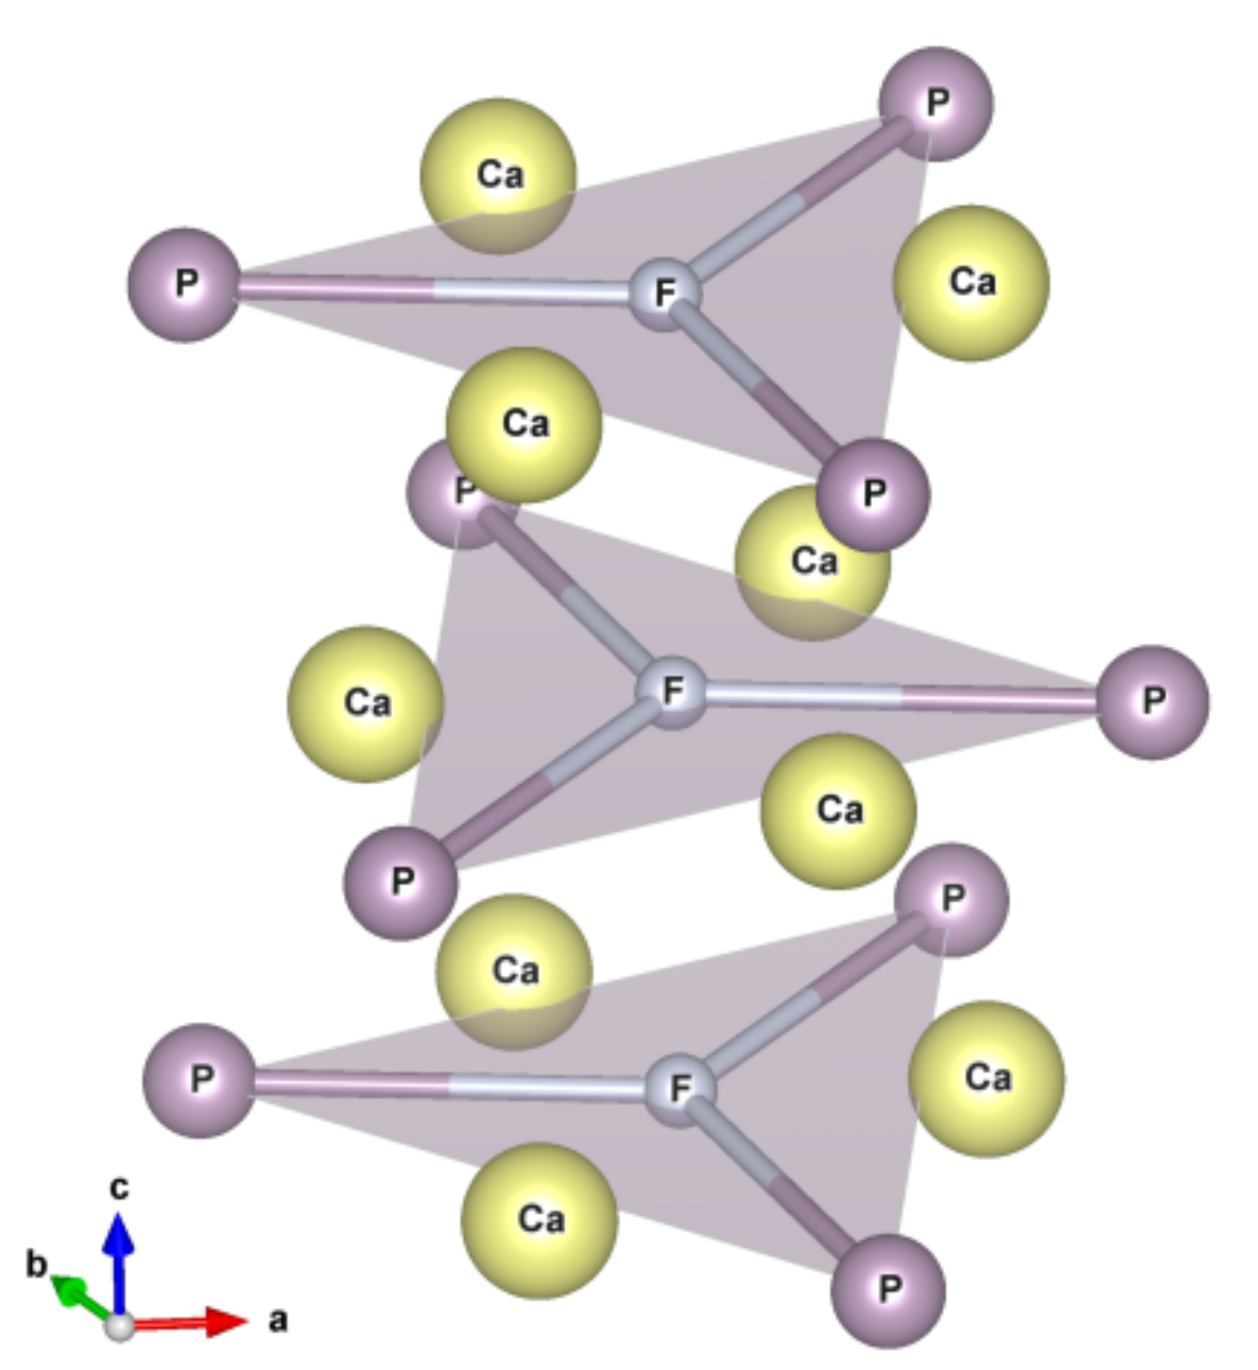
\includegraphics[width=\textwidth]{sample-fap-crystal-structure-part.png}
      \caption{Фтористый апатит Ca$_{10}$(PO$_4$)$_6$F$_2$}
    \end{figure}

    \column{0.6\textwidth}
      Часть кристаллической структуры FAp, показывающая окружение атомов фтора.
      Атомы кислорода были удалены для ясности.
      Атомы фтора равномерно разнесены ($r_{FF}= 3.44$\AA) и расположены в колонны вдоль $c$-оси кристалла.
      Каждый атом фтора окружен тремя равноудаленными атомами фосфора при $r_{FP} = 3.67$\AA,
      которые расположены в вершинах равносторонних треугольников на плоскости, перпендикулярной к $c$-оси,
      а также тремя ионами Ca\textrm{II} на расстоянии $2.34$\AA.
  \end{columns}
\end{frame}
\note{
  Экспериментальные исследования многоквантовой динамики ЯМР одномерных систем были начаты на монокристалле гидроксиапатита кальция Ca5 (PO4)3 F с гексагональной системой ядер фтора.
  Расстояние между соседними цепочками примерно втрое превышает расстояние между ближайшими протонами на цепочке. 
  Это позволяет использовать для интерпретации экспериментальных данных модель изолированной спиновой цепочки.

  В рамках данной модели удается регистрировать двух частичную запутанность, 
  что согласуется с результатами приведёнными в литературе.  
  
  Данная система хорошо описывается моделью ближайших соседей, 
  что плохо сказывается на исследовании многочастичной запутанности. 
  Поэтому больший интерес вызывают системы, в которых взаимодействие со следующими ближайшими соседями значимо. 
}

\begin{frame}{Альтернированная цепочка}
\begin{columns}

    \column{0.3\textwidth}
    \begin{figure}
    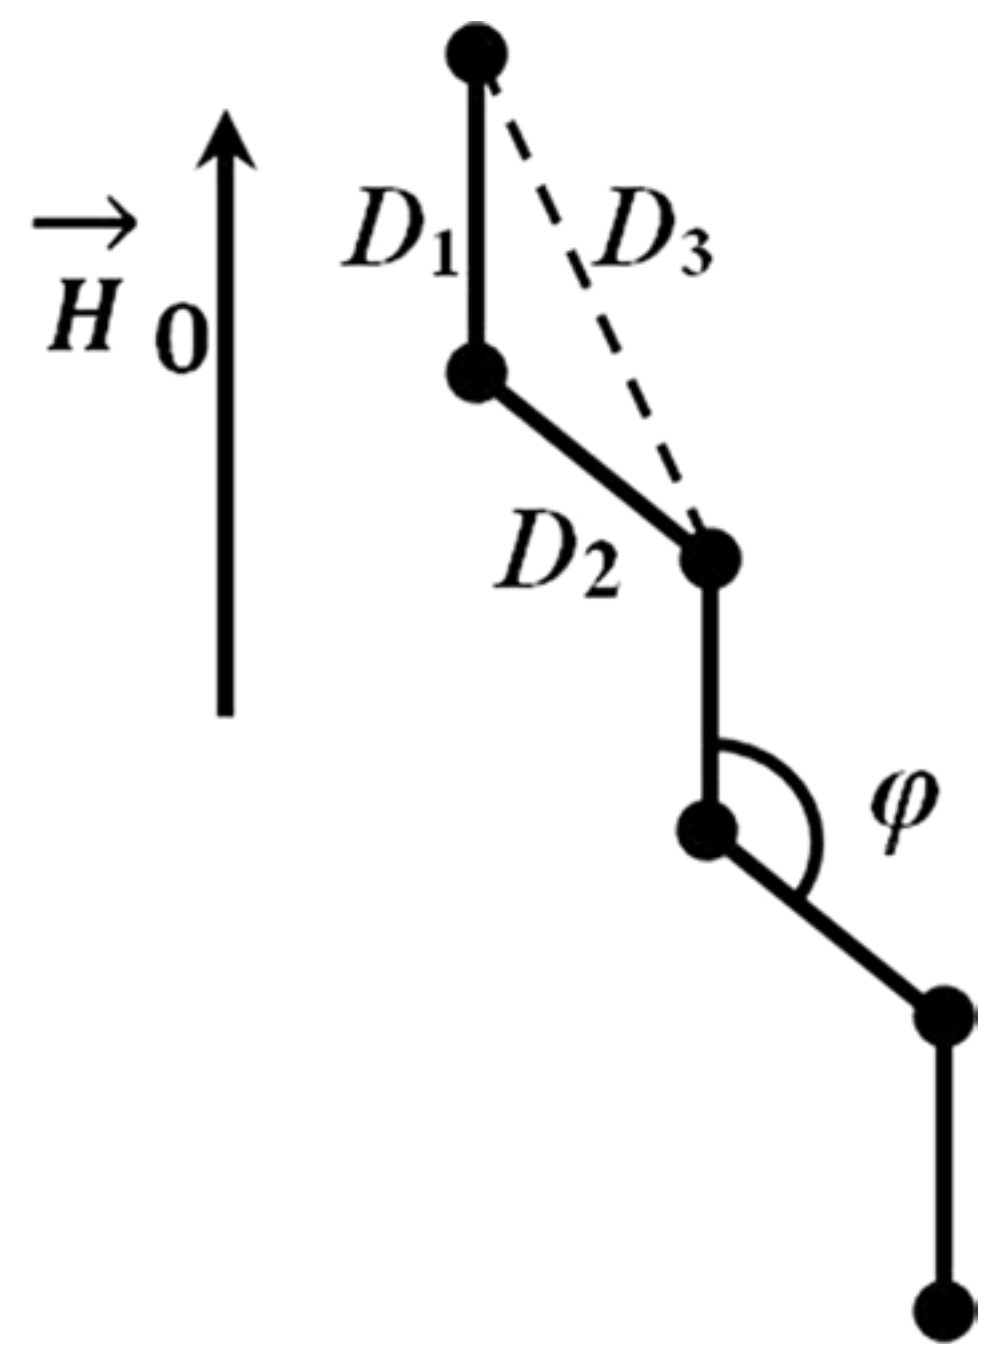
\includegraphics[width=1.0\textwidth]{model-zchain-schema.png}
    \caption{}
    \end{figure}

    \column{0.6\textwidth}
    \begin{block}{Константы взаимодействия}
        $$D_1=\dfrac{\gamma^2\hbar }{r^3}, $$
        $$D_2 = D_1\dfrac{ 3\cos^2 \varphi -1 }{2}, $$
        $$D_3 = D_1 \dfrac{ 3\sin^2 \frac{\varphi}{2} -1}{16 \sin^3, \frac{\varphi}{2}},$$
        где $\gamma$ - гиромагнитное отношение,
        $\varphi$ - угол между соседними связями,
        $r$ - расстояние между соседними спинами в цепочке.
    \end{block}

\end{columns}
\end{frame}
\note{
    Базовый случай это когда одна линия связи направлена вдоль поля. тогда констаты будет самой большой в доль поля.
    Изменяя угол к полю мы можем получить как альтернированную цепочку так и однородную.
    В приближении ближайших и следующих соседей, задача решается аналитически, но она
    не дает полной картины. Поэтому мы решали данную систему численно.
}

\begin{frame}{Альтернированная цепочка}
\begin{columns}

    \column{0.4\textwidth}
    \begin{figure}
      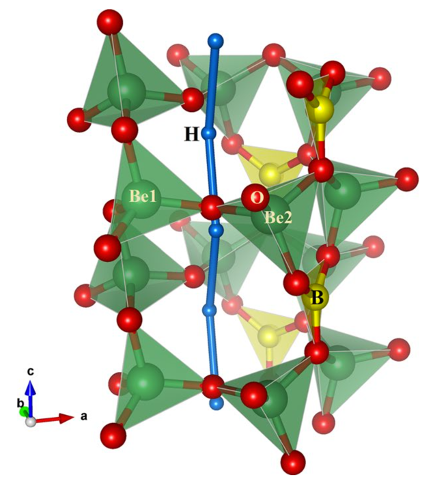
\includegraphics[width=0.85\textwidth]{model-zchain-hambergite-structure.png}
      \caption{}
    %\caption{Hанопора со спин-несущих молекулами во внешнем сильном магнитном поле $\vec B$}
    \end{figure}

    \column{0.6\textwidth}
    \begin{block}{Гамбергит $Be_2BO_3(OH)$\footnote[frame]{
        G.A. Bochkin and et al., \textit{J. Magn. Res.} \textbf{319}, 106816, (2020)} }
        \begin{itemize}
            \item Дипольное взаимодействие между ближайшими спинами протонов в цепи в 17 раз сильнее, чем со спинами окружающих цепей (в худшем случае).
            \item Взаимодействия с остальными окружающими спинами по меньшей мере в 30 раз слабее.
            \item Вклад дипольной связи между спинами в одной и той же цепи доминирует над остальными взаимодействиями.
        \end{itemize}
    \end{block}

\end{columns}
\end{frame}
\note{
    В одномерных цепочках возникают когерентности только $\pm 2$ порядка
    и следовательно дисперсия распределения будет небольшой
    и мы не увидим запутанных кластеров.
    Однако в альтернированная цепочке гамбергита возникают когерентности $\pm 4$ порядка
    и следовательно можно использовать эту модель для исследования многочастичной запутанности.
    The distance to these two protons is 4.49 Å
    The distance between a given chain and surrounding proton chains is at least 2.1 times larger than the distance between neighbors in the chain.

  % JMR 2020
}

% \chapter{Многоспиновая запутанность в зигзагообразной цепочке}
\chapter{Многоспиновая запутанность в квазиодномерных цепочках}
\label{chapter:manayparticle-entantlement-in-zigzag-chain}

В предыдущей главе~\ref{chapter:manyparticle-entanglement-in-nanopore}
была подробно исследована многочастичная запутанность,
возникающая в МК эксперименте ЯМР в нанопоре.
Данная модель показала себя отличной площадкой
для исследования запутанности многих взаимодействующих частиц.
Тем не менее одномерные модели значительно лучше изучены как теоретически,
так и экспериментально~(см. раздел~\ref{sec:model-uniform-chain}).
В этой главе будет исследована многочастичная запутанность,  возникающая в таких системах. Основные результаты этой главы отражены в работах G.A. Bochkin, E.B. Fel'dman, E.I. Kuznetsova, I.D. Lazarev, S.G. Vasil'ev, V.I. Volkov, 1H NMR in a quasi-one-dimensional zig-zag spin chain of hambergite, Be2BO3(OH), \textit{Journal of Magnetic Resonance}, 319:106816, 2020
и
G. A. Bochkin, S. I. Doronin, E. I. Kuznetsova, I. D. Lazarev, E. B. Fel'dman, S. G. Vasil'ev, Many-Spin Entanglement in Zigzag Spin Chain in Multiple Quantum NMR, \textit{Applied Magnetic Resonance}, 51(7):667-678, 2020.



\section{Однородная цепочка}
Однородная цепочка является наиболее простой разновидностью одномерной системы.
Создание запутанных кластеров в таких цепочках ограничено слабыми ДДВ удаленных спинов.
В МК эксперименте ЯМР в однородной цепочке существенны когерентности только нулевого и плюс/минус второго порядков.
Оценка снизу информации Фишера может быть получена с помощью Гауссова приближения для распределения интенсивностей МК когерентностей~\cite{Baum1985}.
В этом случае выражение для МК когерентностей имеет
%
\begin{equation}\label{eq:gaussaprox}
  J(\tau, T)=\dfrac{1}{\sqrt{\pi N_c(T)}} \exp\p{-\frac{n^2}{N_c(T)}},
\end{equation}
%
где $N_c(T)$ -- число коррелированных спинов,
ответственных за создание профиля МК когерентности.
Поскольку удвоенный второй момент интенсивностей МК когерентностей $2M_2(\tau, T)$ является нижней границей квантовой информации Фишера $F_Q$
(см.~раздел~\ref{sec:quantum-fisher-information-mesuarement-at-high-temperature}),
из уравнения~(\ref{eq:gaussaprox}) можно найти, что
%
\begin{equation}\label{eq:qfisheinf}
  F_Q \geq 2M_2(\tau, T) = N_c(T) \geq N,
\end{equation}
%
где $N$ --- число узлов в цепочке.
Для небольших значений $k$ верхнюю границу информации Фишера $k$-сепарабельного состояния
$F^k_Q = \sup{F_Q\p{\rho_{k-\mathrm{prod}}}}$~(см.~раздел.~\ref{sec:manyparticle-entanglement-criteria}) можно переписать в приближённой форме как
%
\begin{equation}\label{eq:inequalityforfq2}
  F^k_Q \leq k N.
\end{equation}
%
Неравенство~(\ref{eq:inequalityforfq2}) не нарушается ни для какого $k > 0$, когда $F_Q = N$,
а для случая $F_Q > N$ детектируется только парная запутанность.
Полученная оценка согласуется с представленными в литературе~\cite{Doronin2007, Feldman2012} результатами.

Из выражения~(\ref{eq:qfisheinf}) также следует,
что увеличение числа узлов цепочки не способствует детектированию запутанных кластеров большего размера, чем двухчастичный.
Тем не менее этого достаточно для передачи МК когерентностей вдоль цепочки~\cite{Bochkin2018qip} и создания запутанности между удаленными концами цепочки~\cite{Lazarev2019}.

% \subsection{Температурная зависимость запутанности удаленных узлов цепочки}
\subsection{Запутанность удаленных узлов цепочки}
\label{subsec:entanglement-of-remote-chain-nodes}
Однородная цепочка является удобной моделью линии связи для передачи квантовых состояний на короткие расстояния.
Типичная схема линии связи (см.~Рис.\ref{fig:model-uchain-schema}) состоит из передатчика (sender $S$),
приемника (reciever $R$)
и линии передачи (transmition line $TL$).
Также ряд протоколов передачи задействуют расширенный приемник (extended reciever $ER$),
на котором применяется специально сконструированное универсальное унитарное преобразование для наилучшего восстановления передаваемой информации~\cite{Feldman2021}.

\begin{figure}[H]
  \centering
  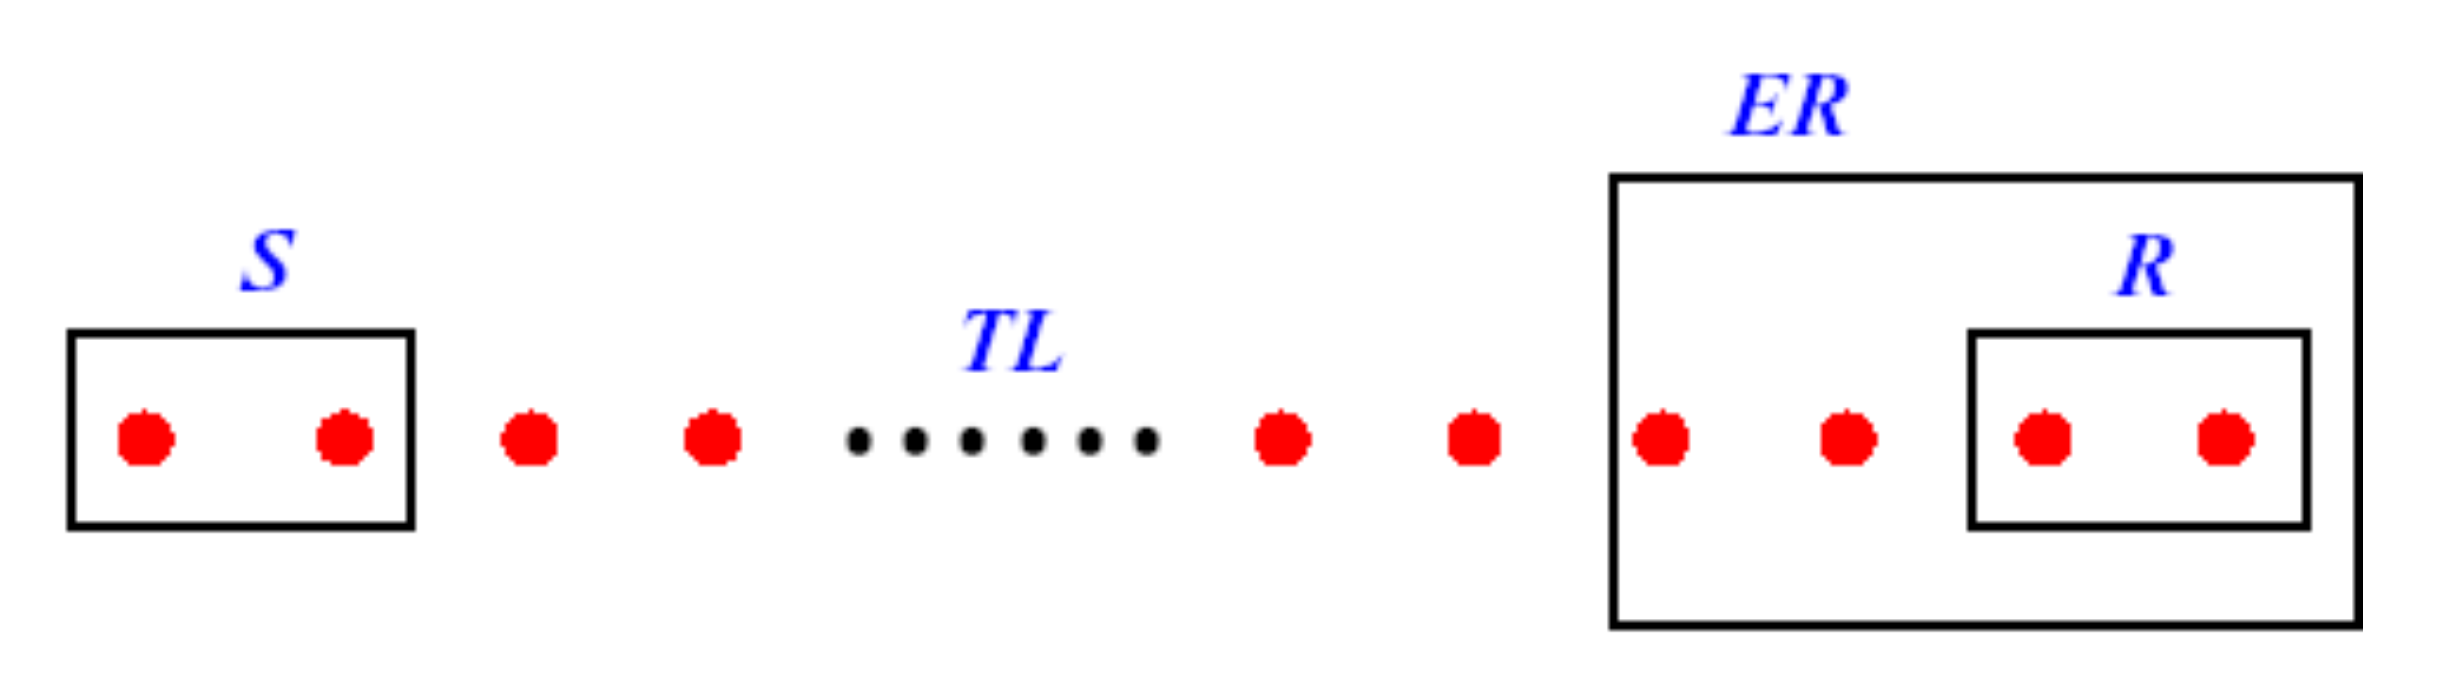
\includegraphics[width=0.9\textwidth]{model-uchain-schema.png}
  \caption{
    Схематичное изображение линии передачи квантовых состояний.
    S --- передатчик,
    TL --- линия передачи,
    ER --- расширенный приемник,
    R --- приемник.
  }
  \label{fig:model-uchain-schema}
\end{figure}

В оригинальной работе Бозе~\cite{Bose2003} был рассмотрен случай передачи однокубитного состояния под действием гейзенберговского гамильтониана.
В рамках МК спектроскопии ЯМР более естественно рассматривать передачу под действием $XX$-гамильтониана,
который для однородной цепочки совпадает с МК гамильтонианом $\hmq$~(\ref{eq:hmq}) с точностью до поворота~(см.~раздел~\ref{sec:model-uniform-chain}).
В приближении ближайших соседей во вращающейся системе координат с Ларморовской частотой $\omega_0$ выражение $XX$-гамильтониана имеет вид:
%
\begin{equation}\label{eq:hxx}
  H_\mathrm{XX} = D\sum_{j=1}^{N-1}\p{I_{j,x}I_{j+1,x} + I_{j,y}I_{j+1,y}},
\end{equation}
где $D$ --- константна ДДВ между соседними узлами,
а N --- число узлов в цепочке.
В базисе бесспиновых фермионных операторов $\gamma_j$ and $\gamma_j ^+$
гамильтониан~(\ref{eq:hxx}) имеет диагональный вид
\begin{equation}\label{Diagonal_Hamiltonian}
  H_\mathrm{XX}=\sum\limits _{k}\varepsilon _{k}\gamma ^{+}_{k}\gamma _{k}.
\end{equation}
Переход к новому базису определяется преобразованием Йордана-Вигнера~\cite{Jordan1928, Feldman1998}:
\begin{equation}\label{eq:jw_operators}
  \gamma _{k}=\sum\limits ^{N}_{j=1}g_{kj} c_{j},
  \quad
  \gamma^+ _{k}=\sum\limits ^{N}_{j=1}g_{kj} c_{j}^+,
\end{equation}
где операторы рождения/уничтожения
\begin{equation}\label{eq:creation_annihilation_operators}
  c_{j}=(-2)^{j-1}I_{1,z}I_{2,z}I_{3,z}...I_{j-1,z}I^-_j,
  \quad
  c_{j}^+=(-2)^{j-1}I_{1,z}I_{2,z}I_{3,z}...I_{j-1,z}I^+_j,
\end{equation}
и
\begin{equation}\label{eq:gammakj}
  \varepsilon_{k} = D \cos(k),
  \quad
  g_{kj} =\sqrt {\frac {2}{N+1}}\sin \left( kj\right),
  \quad
  k=\frac {\pi n}{N+1}\quad n=1\ldots N .
\end{equation}

В общем случае в начальный момент времени однокубитный передатчик --- это произвольное чистое состояние
%
\begin{equation}\label{eq:random-pure-state}
  \ket{\psi_\mathrm{init}} = a\ket{0} + b\ket{1},
  \quad
  |a|^2 + |b|^2 = 1,
\end{equation}
%
а линия передачи и приемник находятся в термодинамическом равновесном состоянии
%
\begin{equation}
    \rho^\mathrm{TL, R}_\mathrm{init} = \otimes_{i=2}^N e^{\beta I_{i, z}}.
\end{equation}

Эволюционная матрица плотности может быть найдена из стационарного уравнения Лиювилля
\begin{equation}\label{eq:eval-rho-liuville}
  \rho(t) = e^{-iH_\mathrm{XX}t}
    \ket{\psi_\mathrm{init}} \bra{\psi_\mathrm{init}}
    \otimes
    \rho^\mathrm{TL, R}_\mathrm{init}
    e^{iH_\mathrm{XX}t}.
\end{equation}
После проведения редукции эволюционной матрицы плотности $\rho(t)$~(\ref{eq:eval-rho-liuville}),
матрица плотности передатчика и приемника определяется выражением
%
\small
\begin{equation}\label{eq:eval-rho-sr}
\rho^\mathrm{S,R}(t) =
\begin{pmatrix}
  \begin{array}{r}
    L(|f|^2+|g|^2) \\
    + \frac{e^{2\beta}}{(e^{\beta}+1)^2}
  \end{array}
  &
  \begin{array}{r}
    -\p{-\tanh\frac{\beta}{2}}^{N-2} \\
    \times \frac{ab^*f^* e^{\frac{\beta}{2}}}{2\cosh\frac{\beta}{2}}
  \end{array}
  &
  \frac{ab^* e^{\beta /2}}{2\cosh\frac{\beta}{2}}g^*
  &
  0\\
  &
  &
  &\\
  \begin{array}{r}
    -\p{-\tanh\frac{\beta}{2}}^{N-2} \\
    \times\frac{a^*bf e^{\frac{\beta}{2}}}{2\cosh\frac{\beta}{2}}
  \end{array}
  &
  \begin{array}{r}
    L(e^{-\beta}|g|^2-|f|^2) \\
    +\frac{1}{2\cosh{\beta}+2}
  \end{array}
  &
  \begin{array}{r}
    {2\p{-\tanh\frac{\beta}{2}}^{n-2}}\\
    \times Lfg^*\cosh\frac{\beta}{2}
  \end{array}
  &
  \frac{ab^* e^{-\beta/2}}{2\cosh\frac{\beta}{2}}g^* \\
  &
  &
  &\\
  \frac{a^*b e^{\beta /2}}{2\cosh\frac{\beta}{2}}g
  &
  \begin{array}{r}
   2\p{-\tanh\frac{\beta}{2}}^{n-2}\\ \times{Lf^*g\cosh\frac{\beta}{2}}
  \end{array}
  &
  \begin{array}{r}
    L(e^{-\beta}|f|^2 -|g|^2) \\
    +\frac{1}{2\cosh{\beta}+2}
  \end{array}
  &
  \begin{array}{r}
    \p{-\tanh\frac{\beta}{2}}^{N-2} \\
    \times \frac{ab^*f^* e^{-\frac{\beta}{2}}}{2\cosh\frac{\beta}{2}}
  \end{array}
  &
  &
  &\\
  0
  &
  \frac{a^*b e^{-\beta /2}}{2\cosh\frac{\beta}{2}}g
  &
  \begin{array}{r}
    \p{-\tanh\frac{\beta}{2}} ^{N-2} \\
    \times \frac{a^*bf e^{-\frac{\beta}{2}}}{2\cosh\frac{\beta}{2}}
  \end{array}
  &
  \begin{array}{r}
    -L e^{-\beta}(|f|^2 +|g|^2)\\
    + \frac{1}{(e^{\beta}+1)^2}
  \end{array}
\end{pmatrix},
\end{equation}
\normalsize
где $f={f_N(t, N)}$, $g={f_N(t, 1)}$, $L=\frac{1-2|b|^2 e^{\frac{\beta}{2}}\cosh\frac{\beta}{2}}{\cosh\frac{\beta}{2}}$
и
%
\begin{equation}
  f_N(t, j) = \frac{2}{N+1}\sum_k e^{i\epsilon_k t}\sin k \sin jk.
\end{equation}

\begin{figure}[H]
  \begin{subfigure}{0.45\textwidth}
    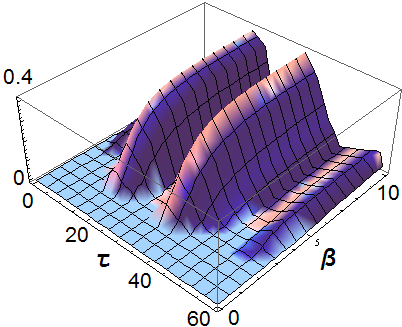
\includegraphics[width=\textwidth]{concurence-temp-uniform-chain-N4.png}
    \caption{
      $\ket{\psi} = \dfrac{\ket{0} + \ket{1}}{\sqrt{2}}$
    }
    \label{fig:concurence-temp-uniform-chain-N4}
  \end{subfigure}
  \hfill
  \begin{subfigure}{0.45\textwidth}
    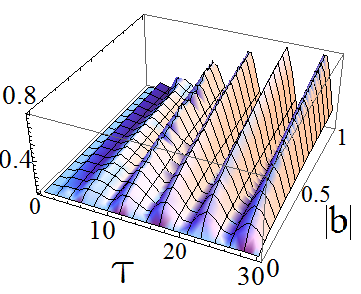
\includegraphics[width=\textwidth]{concurence-polarization-uniform-chain-N4.png}
    \caption{
      $\beta = 5$
    }
    \label{fig:concurence-polarization-uniform-chain-N4}
  \end{subfigure}
  \caption{
    Зависимость согласованности $C$ от безразмерного времени $\tau = Dt$,
    обратной температуры $\beta$
    (cм. Рис.~\ref{fig:concurence-temp-uniform-chain-N4})
    и величины поляризации $|b|$
    (cм. Рис.~\ref{fig:concurence-polarization-uniform-chain-N4})
    при передаче квантового состояния по цепочке из $N=4$ спинов.
  }
  \label{fig:councurence-uniform-chain-N4}
\end{figure}

В качестве критерия запутанности для двухкубитного смешанного состояния удобнее всего использовать критерий Вуттерса~(см. раздел. ~\ref{sec:entanglement-criteria}) на основе согласованности $C$.
Температурная зависимость согласованности $C$ при передаче чистого состояния $\ket{\psi} = \frac{\ket{0} + \ket{1}}{\sqrt{2}}$ ($a=b=\frac{1}{\sqrt{2}}$) представлена на Рис.~\ref{fig:concurence-temp-uniform-chain-N4}.
При обратной температуре $\beta > 1$ приемник и передатчик запутываются.
На Рис.~\ref{fig:concurence-polarization-uniform-chain-N4} представлена зависимость согласованности $C$ от различных значений начальной поляризации передатчика при обратной температуре $\beta = 5$.
Приемник и передатчик запутываются при любой начальной поляризации.

\begin{figure}[H]
    \centering
    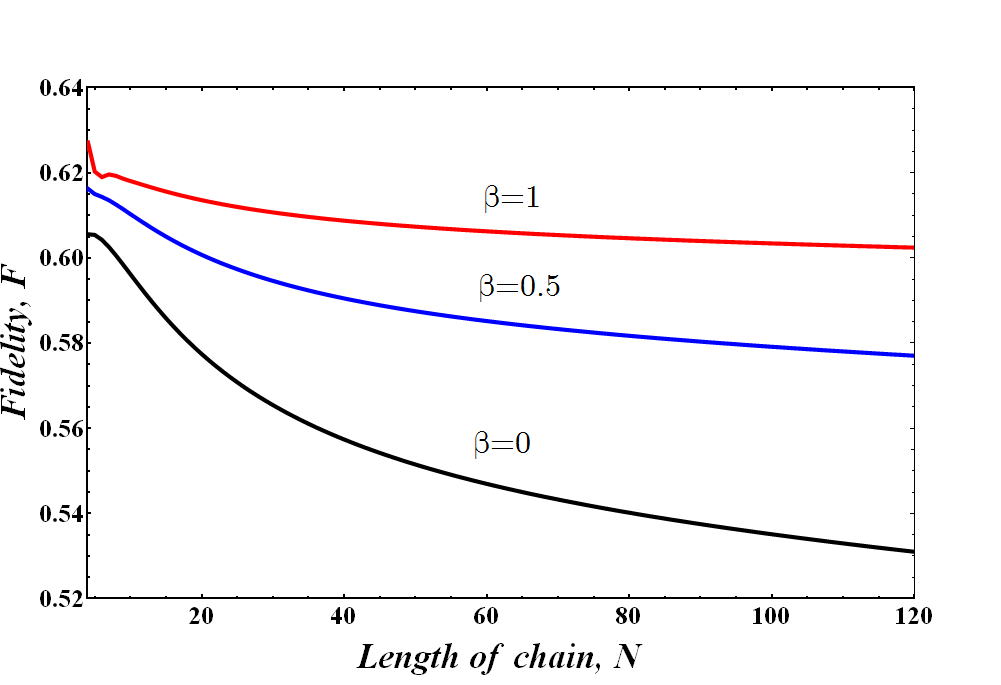
\includegraphics[width=0.8\textwidth]{fidelity-n-beta.png}
    \caption{
      Зависимость фиделити переданного состояния
      $\rho^\mathrm{S}_\mathrm{init}$
      и полученного
      $\rho^\mathrm{R}\p{\bar\tau_N}$
      от количества узлов в цепи.
      Разные линии соответствуют разным значениям обратной температуры $\beta$.
     }
    \label{fig:fidelity-n-beta}
\end{figure}

Идеальная передача произвольного квантового состояния в спиновых цепочках достижима только в очень специфических случаях~\cite{Christandl2004, Karbach2005} и может быть легко разрушена небольшими возмущениями гамильтониана взаимодействия.
В общем случае передача осуществляться не идеально,
но с высокой вероятностью.
Качество передачи можно оценить с помощью фиделити~\cite{Jozsa1994}
%
\begin{equation}\label{generalFidelity}
  F\p{\rho^\mathrm{S}_\mathrm{init}, \rho^\mathrm{R}\p{t}}
  = \tr{\rho^\mathrm{S}_\mathrm{init}, \rho^\mathrm{R}(t)}.
\end{equation}
%
С учетом $\rho^\mathrm{R}\p{t} = \tr{\rho^\mathrm{S,R}(t)}_\mathrm{S}$,
аналитическое выражение для фиделити имеет вид
%
\begin{multline}\label{exactfidelity}
  F\p{\rho^\mathrm{S}_\mathrm{init}, \rho^\mathrm{R}\p{t}}
  = (1-2|b|^2)\p{
    \frac{e^{\beta/2}}{\cosh \beta/2}
    + \p{\frac{e^{-\beta/2}}{\cosh \beta/2} -|b|^2 }
      \left|f_N(t, N)\right|^2
  } \\
  + |b|^2
  + 2 |b|^2 \p{1-|b|^2} \Re\left\{f_N(t, N)\right\}
  \p{-\tanh \p{\frac{\beta}{2}}}^{N-1}.
\end{multline}
%
Время $\bar\tau_{N}$, при котором фиделити достигает первого пика, называется временем передачи~\cite{Feldman2016}.
Оно совпадает с временем первого пика функции $\left|f_N(t, N)\right|^2$.
Фиделити~\cite{Jozsa1994} переданного и полученного квантового состояния в момент времени $\bar\tau_{N}$ уменьшается с увеличением длинны цепочки (см. Рис.\ref{fig:fidelity-n-beta}).


\subsection{Идеальная передача запутанных состояний}
% \subsection{Идеальная передача МК когерентности нулевого порядка}

гамильтониан $H_\mathrm{XX}$ коммутирует с $z$-проекцией $I_z$ полного спинового момента
и сохраняет число возбуждений в процессе эволюции.
В этом случае когерентности разных порядков не перемешиваются~\cite{Feldman2017} и могут быть рассмотрены отдельно~\cite{Bochkin2018qip}.
В частности, было показано~\cite{Feldman2021},
что специальная форма когерентности нулевого порядка может передаваться без потерь
по цепочке из $N$ узлов, находящейся в основном состоянии:
%
\begin{equation}
  \rho^\mathrm{TL}_\mathrm{init} = \otimes^{N_\mathrm{TL}}_{i=1}\ket{0},
  \quad
  \rho^\mathrm{R}_\mathrm{init} = \otimes^{N_\mathrm{R}}_{i=1}\ket{0},
\end{equation}
%
где $N_\mathrm{R}$ --- количество кубитов в приёмнике,
а $N_\mathrm{TL}  = N - 2 N_\mathrm{R}$.
В случае, когда количество кубитов в передатчике $N_\mathrm{S} = N_\mathrm{R} = 3$,
специальная матрица плотности передатчика,
которая может быть передана без потерь,
в базисе с одним возбуждением
$\left \{\ket{000}, \ket{001}, \ket{010}, \ket{100} \right\}$
может быть записана в виде
%
\begin{equation}
  \rho^\mathrm{S}_\mathrm{init} =
  \begin{pmatrix}
    u &    0     &    0    & 0 \\
    0 &   x_1    & \omega  & 0 \\
    0 & \omega^* &   x_2   & 0 \\
    0 &    0     &    0    & v
  \end{pmatrix}.
\end{equation}
%
После редукции $\rho^\mathrm{S}_\mathrm{init}$ по первому спину
матрица плотности оставшихся двух в полном базисе имеет вид
\begin{equation}\label{eq:rho-s-reduced}
  \tr{\rho^\mathrm{S}_\mathrm{init}}_{1} =
  \begin{pmatrix}
    u + v &    0     &    0    & 0 \\
    0     &   x_1    & \omega  & 0 \\
    0     & \omega^* &   x_2   & 0 \\
    0     &    0     &    0    & 0
  \end{pmatrix}.
\end{equation}
Для матрицы вида~(\ref{eq:rho-s-reduced}) согласованность $C$
определяется~(cм.~раздел~\ref{sec:entanglement-criteria}) только величиной недиагональных элементов:
%
\begin{equation}
  C = 2 |w|.
\end{equation}


\begin{figure}[H]
    \centering
    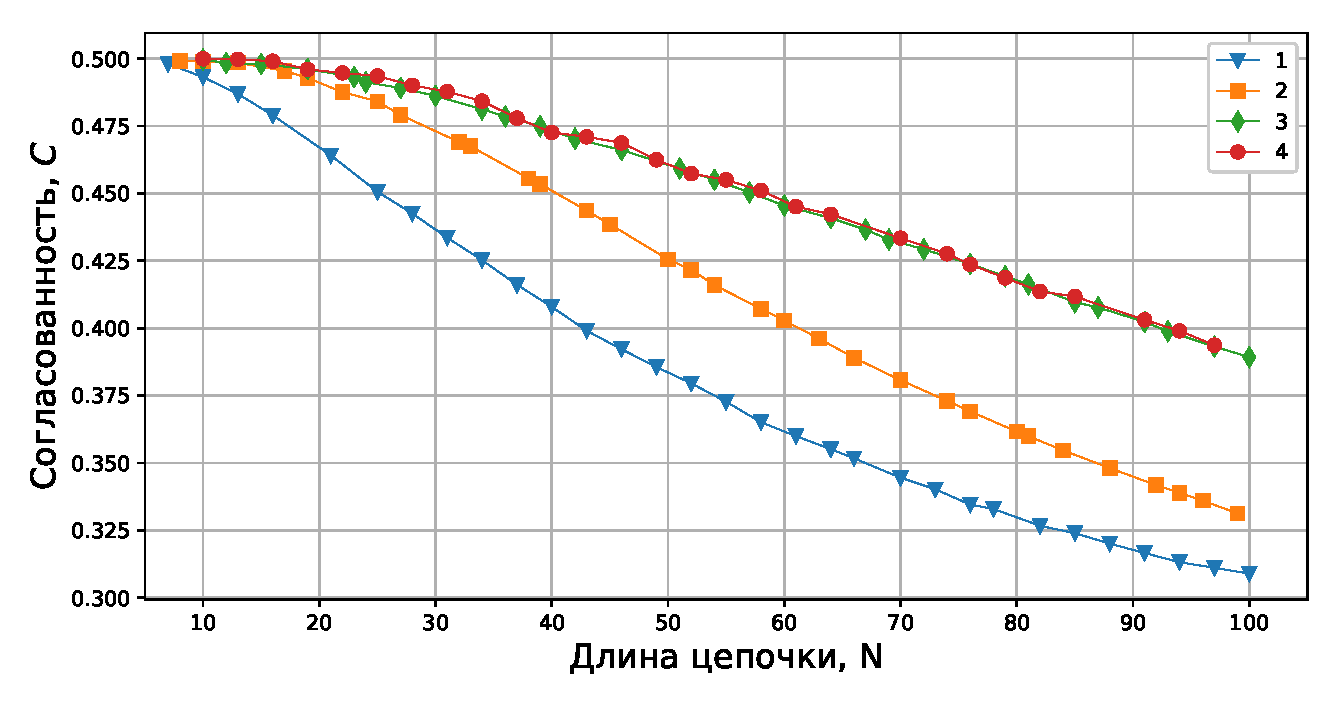
\includegraphics[width=0.9\textwidth]{concurence-n-s3.eps}
    \caption{
      Максимальное значение согласованности второго и третьего спинов передатчика, состояние которого может быть передано без потерь,
      от количества узлов в цепи.
      Разные линии отвечают разным размерам расширенного приемника.
    }
    \label{fig:concurence-n-s3}
\end{figure}


Так как элементы матрицы плотности, вносящие вклад в каждую когерентность, перемешиваются в процессе эволюции,
на расширенном приемнике ER применятся специальное унитарное преобразование $U^\mathrm{ER}(\phi)$ для их распутывания~\cite{Feldman2017}.
По аналогии с работой~\cite{Bochkin2022} можно подобрать такое унитарное преобразование на расширенном приемнике,
которое позволяет передавать состояния с максимальным значением согласованности второго и третьего спинов передатчика.
На Рис.~\ref{fig:concurence-n-s3} приведены максимально возможные значения согласованности от длины цепочки,
полученные путем максимизации модуля недиагонального элемента $\omega$ матрицы плотности $\rho^\mathrm{S}_\mathrm{init}$ по параметрам унитарного преобразования $U^\mathrm{ER}(\phi)$.
Вычисления выполнены с помощью метода дифференциальной эволюции~\cite{Storn1997,Wormington1999,Lampinen2002} из библиотеки SciPy~\cite{SciPy} версии 1.4.1.


\section{Зигзагообразная цепочка}

\begin{wrapfigure}{O}{0.5\textwidth}
    \centering
    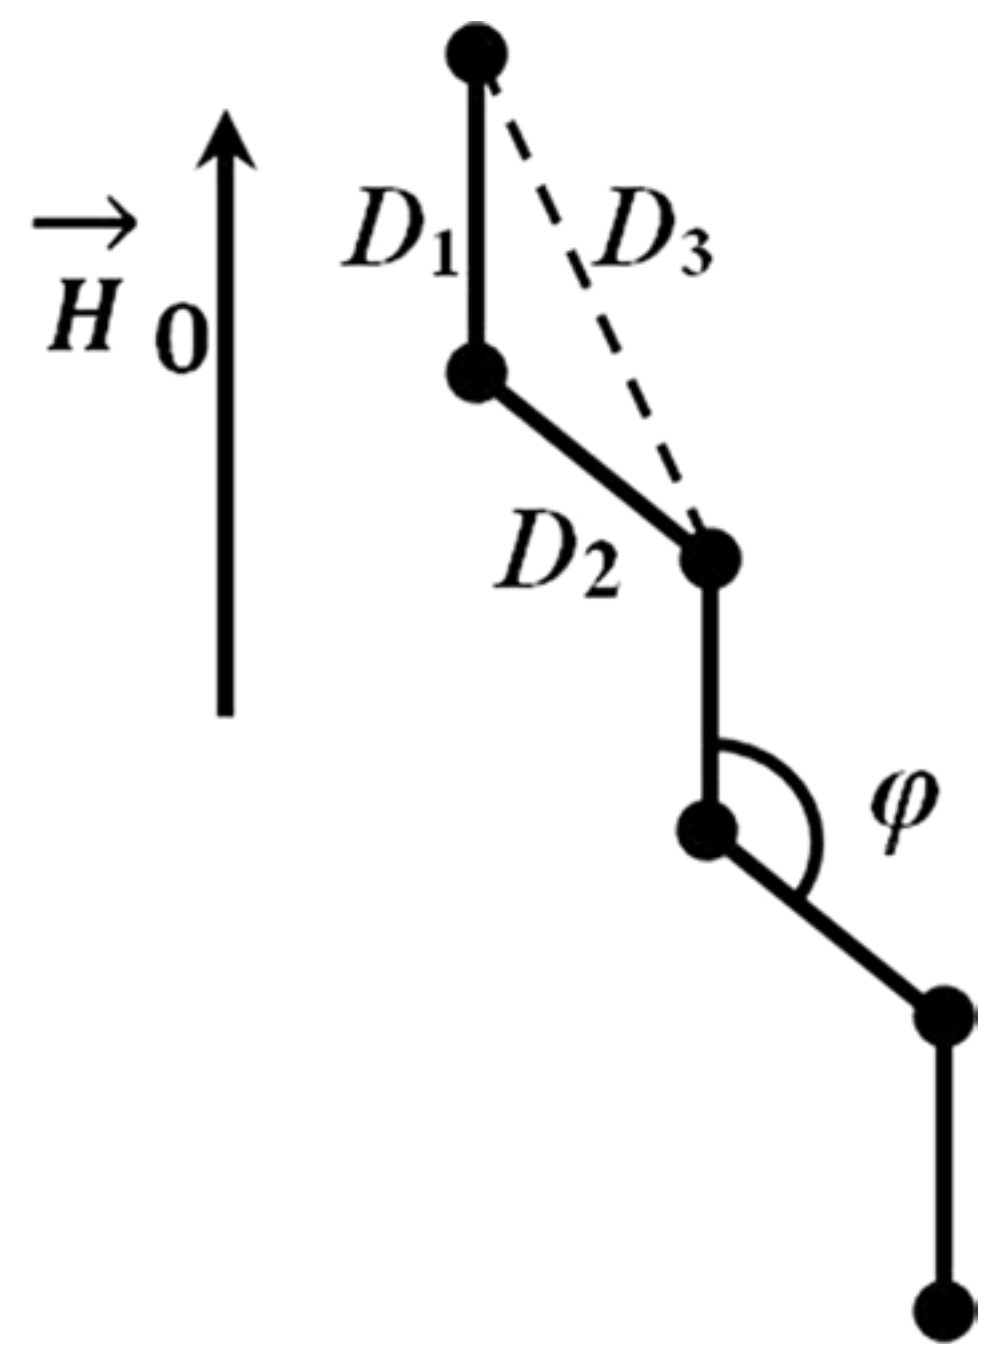
\includegraphics[width=0.3\textwidth]{model-zchain-schema}
    \caption{\protectСхема зигзагообразной цепочки ядерных спинов.
Нечетные звенья параллельны внешнему магнитному полю $\vec{H}_0$,
а $\varphi$ --- угол между соседними звеньями.
% Константы связи $D_1$ и $D_2$ определяются уравнением~(\ref{eq:dipolaconstantsnearest}), а $D_3=D_{n, n+2},\, (n=1,2,...)$
% уравнением~(\ref{eq:dipolaconstantsnextnearest}).
}
    \label{fig:model-zchain-schema}
\end{wrapfigure}

В зигзагообразных цепочках в кристалле гамбергита в МК эксперименте ЯМР,
в отличие от однородных цепочек,
существенны когерентности плюс/минус четвертого порядка (см. раздел~\ref{sec:model-zigzag-chain}).
Данное обстоятельство является важным для исследования многоспиновой запутанности,
поскольку при этом используется второй момент распределения МК когерентностей ЯМР.

На Рис.~\ref{fig:model-zchain-schema} схематично представлена
зигзагообразная цепочка ядерных спинов в сильном внешнем магнитном поле $\vec{\mathcal H}_0$.
Нечетные звенья цепочки параллельны внешнему магнитному полю $\vec{\mathcal H}_0$,
а $\varphi$ - угол между соседними звеньями.
гамильтониан $\hmq$,
описывающий МК динамику ЯМР~(см. раздел~\ref{sec:mq-nrm-experiment}),
задается выражением~\cite{Doronin2000}
%
\begin{equation}\label{hmq-next-nearest}
  \hmqZChainNextNearest = \hmqZChainNextNearestDefinition,
\end{equation}
%
\hmqZChainNextNearestExplanatoryNote
%
Константы диполь-дипольного взаимодействия (ДДВ)
в зигзагообразной цепочке определяются выражениями~\cite{Abragam1982}
%
\begin{equation}\label{eq:dipolaconstantsnearest}
  D_{2n-1, 2n} = D_1 =\dfrac{\gamma^2\hbar }{r^3},
  \quad
  D_{2n, 2n+1} = D_2=\dfrac{\gamma^2\hbar }{2r^3}\p{3\cos^2 \varphi -1},
  \quad
  n=1,2\dots,
\end{equation}
где $\gamma$ -- гиромагнитное отношение,
и $r$ -- расстояние между ближайшими спинами в цепочке.
Также в гамильтониане учитываются взаимодействия со следующими соседями,
константа диполь-дипольного взаимодействия которых определяется как~\cite{Abragam1982}
%
\begin{equation}\label{eq:dipolaconstantsnextnearest}
  D_{n, n+2}=\dfrac{\gamma^2\hbar }{16r^3 \sin^3 \frac{\varphi}{2}}\p{3\sin^2 \frac{\varphi}{2} -1}.
\end{equation}
%
В частности, уравнения~(\ref{eq:dipolaconstantsnearest}),~(\ref{eq:dipolaconstantsnextnearest}) означают,
что для прямой спиновой цепочки, когда  $(\varphi=\pi)$,
константа дипольной связи для ближайших соседей в восемь раз больше,
чем константа дипольной связи между следующими ближайшими соседями.
Тем не менее при $\varphi=\frac{2\pi}{3}$ отношение констант связи
\begin{equation}
  \left|\dfrac{D_{2n, 2n+1}}{D_{2n-1, 2n+1}}\right| = \dfrac{3\sqrt{3}}{5},
\end{equation}
и, следовательно,
диполь-дипольные взаимодействия следующих ближайших соседей
существенны для МК динамики ЯМР при определённых ориентациях зигзагообразной спиновой цепочки
по отношению к направлению внешнего сильного магнитного поля.


\subsection{Температурная зависимость многочастичной запутанности}

\begin{figure}[H]
  \begin{subfigure}[t]{0.31\textwidth}
    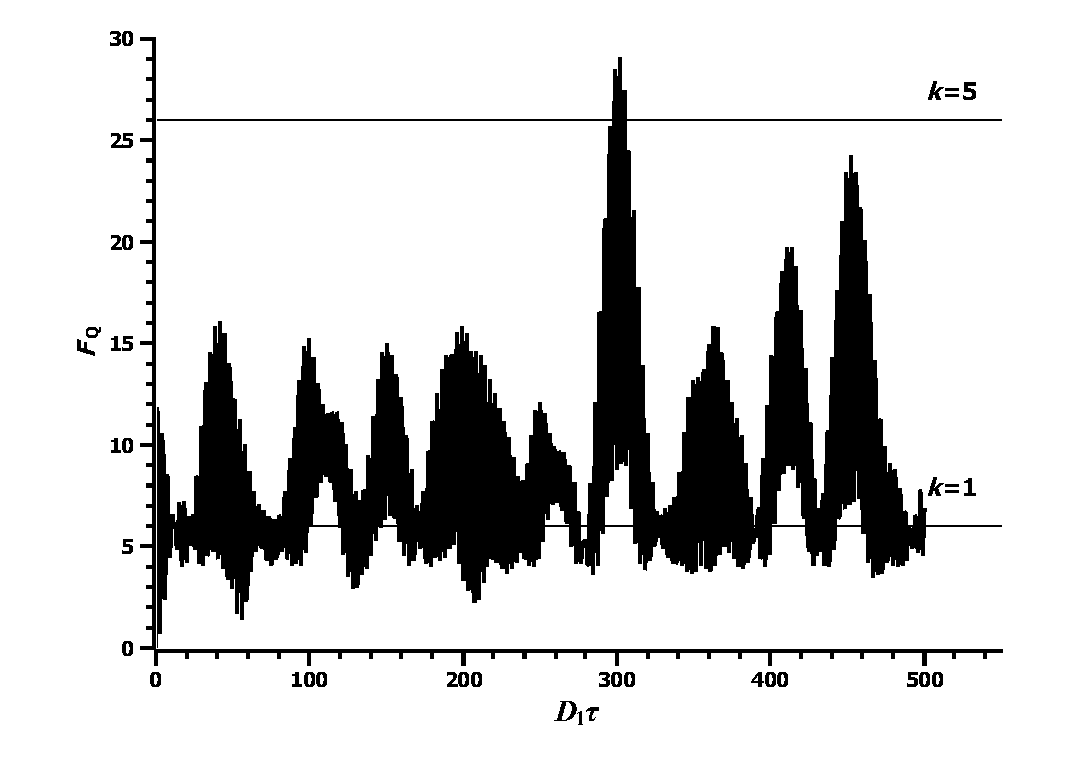
\includegraphics[width=\textwidth]{result-zchain-m2-by-time-n6-beta10}
    \caption{\protect$\beta=10$ ($T = 2.4\times 10^{-3}$~К), $N=6$.
В области выше горизонтальной линии $k=1$ детектируется парная запутанность, выше $k=5$ --- шестиспиновая запутанность.
}
    \label{fig:result-zchain-m2-by-time-n6-beta10}
  \end{subfigure}
  \hfill
  \begin{subfigure}[t]{0.32\textwidth}
    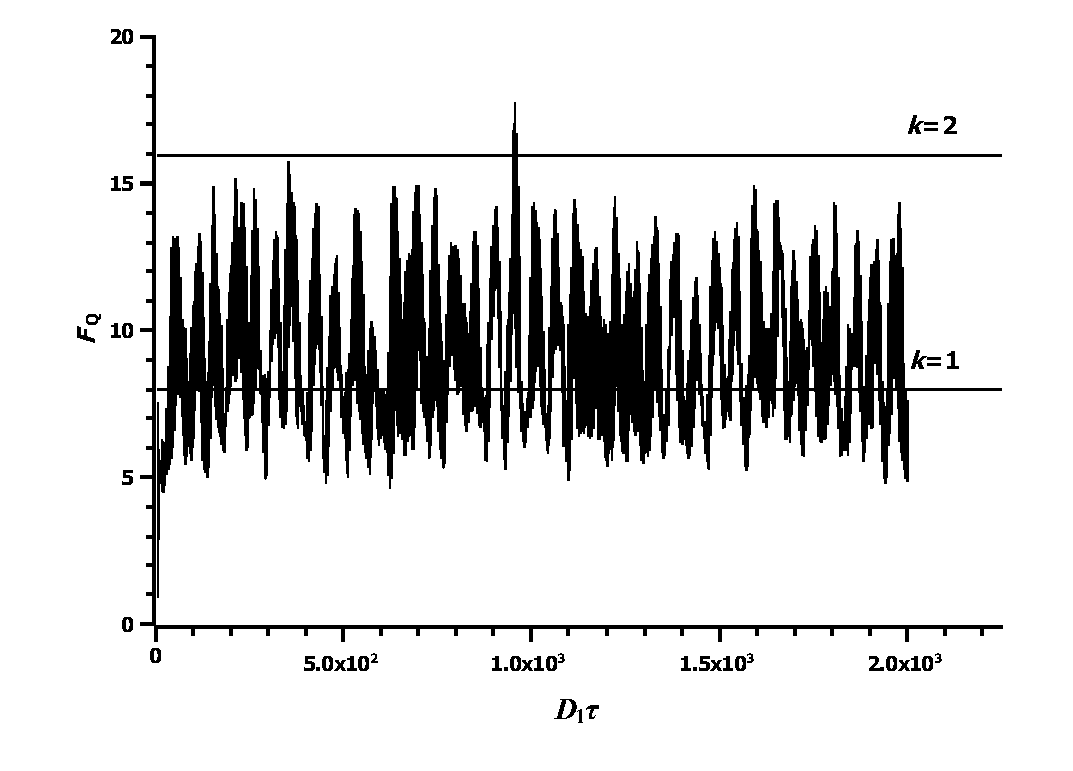
\includegraphics[width=\textwidth]{result-zchain-m2-by-time-n8-beta1}
    \caption{\protect$\beta = 1$ ($T = 2.4\times 10^{-2}$~К), $N=8$.
В области ограниченной горизонтальными линиями $k=1$ и $k=2$
детектируется парная запутанность.
}
    \label{fig:result-zchain-m2-by-time-n8-beta1}
  \end{subfigure}
  \hfill
  \begin{subfigure}[t]{0.31\textwidth}
    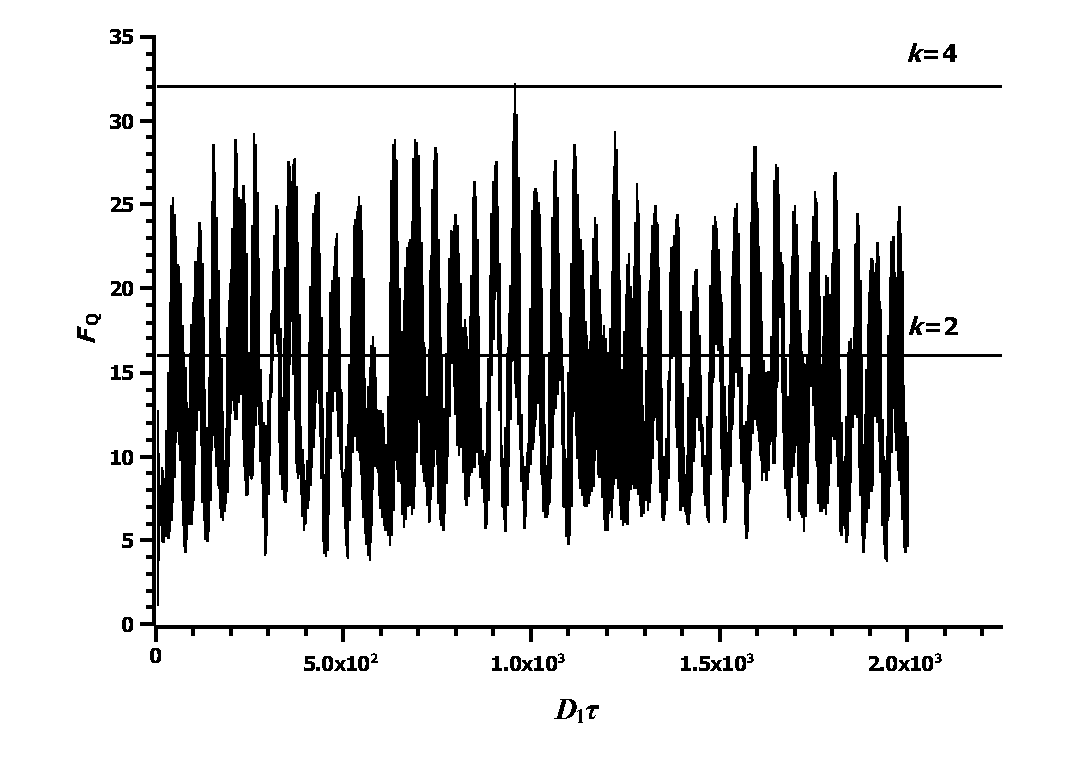
\includegraphics[width=\textwidth]{result-zchain-m2-by-time-n8-beta20}
    \caption{\protect$\beta = 20$ ($T = 1.2\times 10^{-3}$~К), $N=8$.
В области ограниченной горизонтальными линиями $k=2$ и $k=4$
детектируется трехчастичная запутанность.
}
    \label{fig:result-zchain-m2-by-time-n8-beta20}
  \end{subfigure}
  \caption{\protectЗависимость нижней границы квантовой информации Фишера~$F_Q=2M_2(\tau, \beta)$
от безразмерного времени~$D_1\tau$
в зигзагообразной цепочке.
% Горизонтальные линии соответствуют максимальным значениям информации Фишера $k$-разделимых состояний.}
  \label{fig:result-zchain-m2-by-time-ns-betas}
\end{figure}

Для исследования температурной зависимости многочастичной запутанности
в зигзагообразных цепочках
в этом разделе будет рассмотрена МК динамика ЯМР
на подготовительном периоде МК эксперимента ЯМР~(см. раздел~\ref{sec:mq-nrm-experiment})
с начальным термодинамическим равновесным состоянием $\rho_\mathrm{eq}$.
Матрица плотности системы в начальный момент времени имеет вид:
\begin{equation}
  \rho(0, \beta)
  = \rho_\mathrm{eq}
  = \dfrac{e^{\frac{\hbar\omega_{0}}{kT} I_z}}{Z},
  = \dfrac{e^{\beta I_z}}{Z},
\end{equation}
где $Z = \tr{e^{\beta I_z}}$ --- статистическая сумма,
$\hslash$ и $k$ --- константы Планка и Больцмана,
$\omega_{0}$ --- частота Лармора,
$I_\mathrm{z}$ ---  оператор проекции полного углового спинового момента  на ось~$z$,
который направлен вдоль сильного внешнего магнитного поля.

Интенсивности приведенных МК когерентностей ЯМР определяются уравнением~(\ref{eq:reduced-mq-coherences})~(см. раздел~\ref{sec:reduced-mq-coherences}).
Для $\beta=0.5$,
что соответствует температуре $T=4.8 \times 10^{-2}\,\mbox{K}$
при Ларморовской частоте $\omega_0=2\pi\times 500\times 10^6 \,\mbox{s}^{-1}$,
было обнаружено,
что неравенство~(\ref{eq:entanglement-criteria}) может быть выполнено только при $k=1$ для спиновых цепочек с $N=6$ и $N=8$.
Это означает, что в высокотемпературном случае~\cite{Doronin2019}
детектируется парная запутанность,
что согласуется с работой~\cite{Feldman2012}.

% \begin{figure}[H]
%   \begin{subfigure}[t]{0.49\textwidth}
%     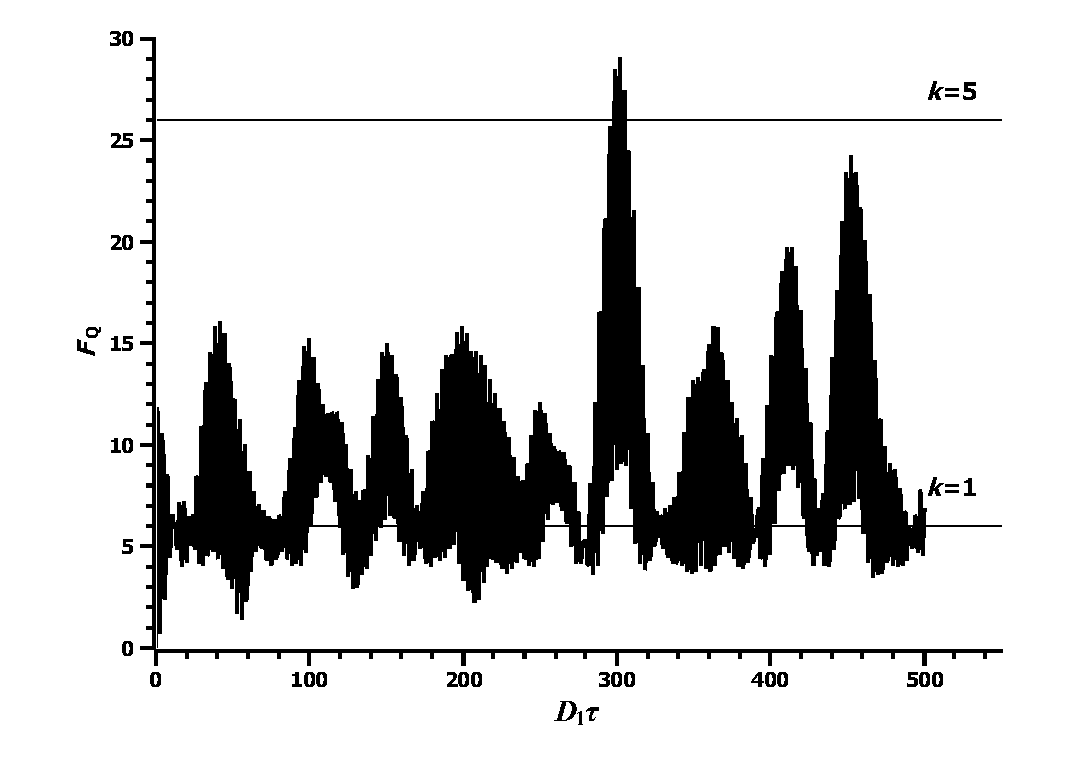
\includegraphics[width=\textwidth]{result-zchain-m2-by-time-n6-beta10}
%     \caption{
%       Зависимость нижней границы квантовой информации
%       Фишера~$F_Q=2M_2(\tau, T)$
%       от безразмерного времени~$D_1\tau$
%       для зигзагообразной цепочки из 6 спинов
%       при температуре $2.4\times 10^{-3}\,\mbox{K}$ $(b=10)$.
%       В области выше горизонтальной линии $k=1$
%       гарантировано существует как минимум парная запутанность.
%       В области выше горизонтальной линии $k=5$
%       гарантировано существует шестиспиновая запутанность.
%     }
%     \label{fig:result-zchain-m2-by-time-n6-beta10}
%   \end{subfigure}
%   \hfill
%   \begin{subfigure}[t]{0.49\textwidth}
%     
\includegraphics[width=\textwidth]{result-zchain-nent-by-n-beta10}
%     \caption{
%       Зависимость оценки максимального количества запутанных спинов $N_{ent}$ от длины цепочки при температуре $2.4\times 10^{-3}\,\mbox{K}$.
%     }
%     \label{fig:result-zchain-nent-by-n-beta10}
%   \end{subfigure}
%   \caption{}
% \end{figure}

Зависимости многоспиновой запутанности от длины цепочки $N$ и температуры исследованы для спиновых цепочек с $4\leqslant N \leqslant 12$.
Временная эволюция нижней границы квантовой информации Фишера,
соответствующая  удвоенному второму моменту распределения интенсивностей МК когерентностей для шестиспиновой цепочки представлена на Рис.~\ref{fig:result-zchain-m2-by-time-n6-beta10} при температуре $2.4\times 10^{-3}\,\mbox{K}$ $(\beta=10)$.
На Рис.~\ref{fig:result-zchain-m2-by-time-n6-beta10} видна полоса,
в которой неравенство~(\ref{eq:entanglement-criteria}) может быть удовлетворено при $1\leqslant k \leqslant 5$.
Таким образом, существует многоспиновая запутанность в спиновых кластерах, состоящих из 2-6 спинов при температуре $2.4\times 10^{-3}\,\mbox{K}$.
Зависимость оценки максимального количества запутанных спинов от длины цепи приведена на Рис.~\ref{fig:result-zchain-nent-by-n-beta10} при температуре $2.4\times 10^{-3}\,\mbox{K}$.

% \begin{figure}[H]
%   \begin{subfigure}[t]{0.49\textwidth}
%     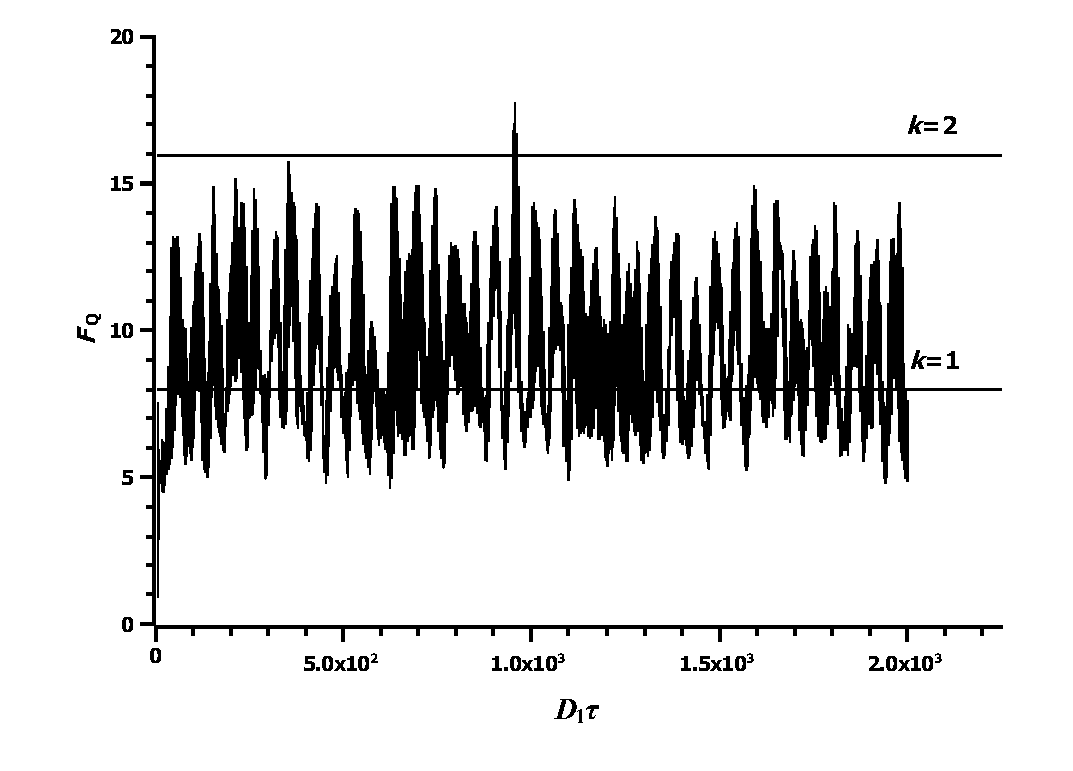
\includegraphics[width=\textwidth]{result-zchain-m2-by-time-n8-beta1}
%     \caption{
%       При температуре $2.4\times 10^{-2}\,\mbox{K}$
%       в области ограниченной горизонтальными линиями $k=1$ и $k=2$
%       присутствует как минимум парная запутанность.
%     }
%     \label{fig:result-zchain-m2-by-time-n8-beta1}
%   \end{subfigure}
%   \hfill
%   \begin{subfigure}[t]{0.49\textwidth}
%     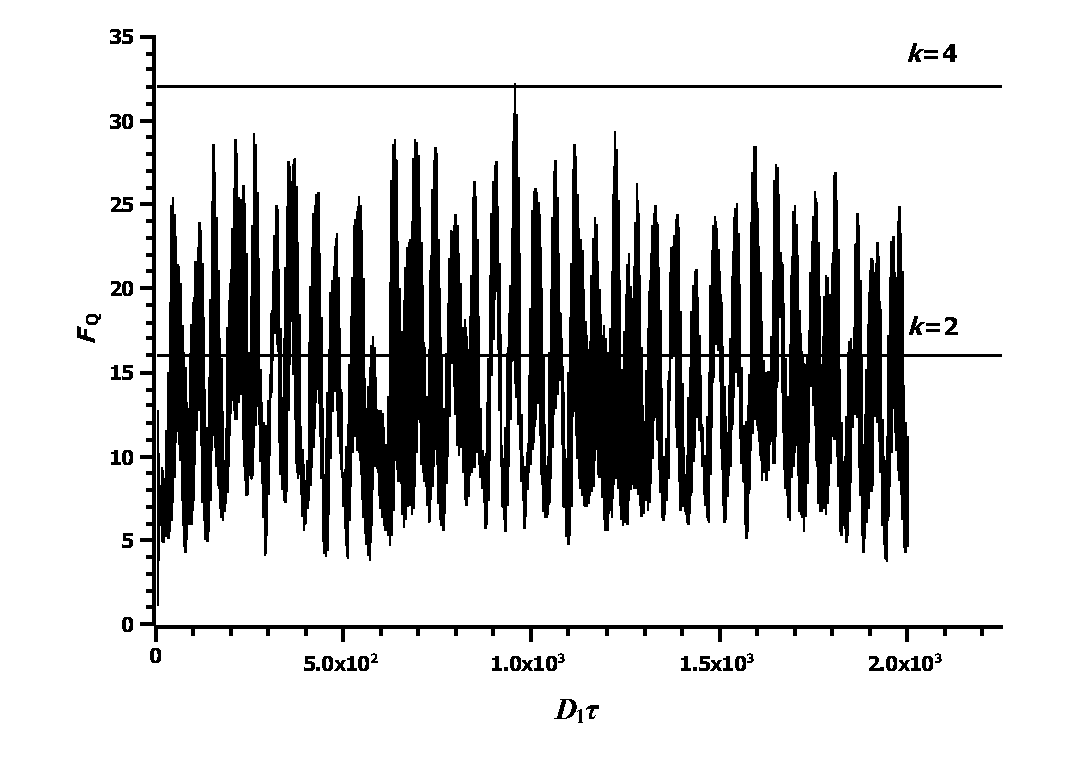
\includegraphics[width=\textwidth]{result-zchain-m2-by-time-n8-beta20}
%     \caption{
%        При температуре $1.2\times 10^{-3}\,\mbox{K}$
%        в области ограниченной горизонтальными линиями $k=2$ и $k=4$
%        наблюдается как минимум трехчастичная запутанность.
%     }
%     \label{fig:result-zchain-m2-by-time-n8-beta20}
%   \end{subfigure}
%   \caption{
%     Временная эволюция нижней границы информации Фишера~$F_Q=2M_2(\tau, T)$
%     от безразмерного времени~$D_1\tau$
%     в восьмиспиновой зигзагообразной цепочке.
%   }
% \end{figure}


\begin{figure}[H]
  \begin{subfigure}[t]{0.48\textwidth}
    \centering
    
\includegraphics[width=\textwidth]{result-zchain-nent-by-n-beta10}
    \caption{}
    % \caption{\protectЗависимость максимального задетектированного размера запутанного кластера~$N_{ent}$ от длины цепочки $N$ при температуре $\beta = 10$ ($T = 2.4\times 10^{-3}$~К).
}
    \label{fig:result-zchain-nent-by-n-beta10}
  \end{subfigure}
  \hfill
  \begin{subfigure}[t]{0.48\textwidth}
    \centering
    
\includegraphics[width=\textwidth]{result-zchain-nent-by-beta-n8-n6}
    \caption{}
    % \caption{\protectЗависимость максимального измеренного числа запутанных спинов~$N_{ent}$ от обратной температуры $\beta$
в зигзагообразной цепочке,
состоящей из шести и восьми спинов.}
    \label{fig:result-zchain-nent-by-beta-n8-n6}
  \end{subfigure}
  \label{fig:result-zchain-nent-by-betaand-n}
  \caption{\protect Зависимость максимального числа запутанных спинов~$N_{ent}$ от
\subref{fig:result-zchain-nent-by-n-beta10}) длины зигзагообразной цепочки $N$ при температуре $\beta = 10$ ($T = 2.4\times 10^{-3}$~К);
\subref{fig:result-zchain-nent-by-beta-n8-n6}) температуры $\beta$ в зигзагообразной цепочке, состоящей из шести и восьми спинов.}
\end{figure}


% \begin{wrapfigure}{O}{0.5\textwidth}
%   \centering
%   
\includegraphics[width=0.5\textwidth]{result-zchain-nent-by-beta-n8-n6}
%   \caption{
%     Зависимость оценки максимального числа запутанных спинов от обратной температуры $b$
%     для зигзагообразной цепочки,
%     состоящей из шести и восьми спинов.
%     }
%     \label{fig:result-zchain-nent-by-beta-n8-n6}
% \end{wrapfigure}

Временная эволюция восьмиспиновой зигзагообразной цепочки представлена при $T=2.4\times 10^{-2}\,\mbox{K}$ (Рис.~\ref{fig:result-zchain-m2-by-time-n8-beta1}) и $T=1.2\times 10^{-2}\,\mbox{K}$ (Рис.~\ref{fig:result-zchain-m2-by-time-n8-beta20}).  Видно, что при температуре $T=2.4\times 10^{-2}\,\mbox{K}$ возникают многоспиновые запутанные кластеры, состоящие из двух или трех спинов, а при температуре $T=1.2\times 10^{-2}\,\mbox{K}$ возникают кластеры с $2\leqslant k \leqslant 5$.
Число запутанных спинов увеличивается с понижением температуры.

Зависимость числа запутанных спинов от температуры для зигзагообразных цепочек,
состоящих из шести или восьми спинов, приведена на Рис.~\ref{fig:result-zchain-nent-by-beta-n8-n6}.
% В этих цепочках почти все спины запутаны при низких температурах.
Так же как и в случае системы эквивалентных спинов,
при низких температурах почти все спины в цепочке запутанны.
% Результаты получены на небольшом интервале времени,
% поэтому эффектами декогеренции можно пренебречь.


% The creation of entangled clusters in the considered zigzag chains is limited by weak DDIs of remote spins.  Accordingly, that process requires a large time interval. Practically, the role of decoherence gets very important in that case.  We note also that the analysis of the inequality \eqref{inequalityforfq} shows that an increase in chain length does not result in an increase of the number of the entangled spins even at long times. Indeed, we can rewrite \eqref{inequalityforfq} in the approximate simple form
% \begin{equation}\label{inequalityforfq2}
% F_Q>k N.
% \end{equation}
% In order to estimate the Fisher information we use the Gaussian approximation for the distribution of the intensities of MQ coherences \cite{baum}
% \begin{equation}\label{gaussaprox}
% J(\tau, T)=\dsfrac{1}{\sqrt{\pi N_c(T)}} \exp\p{{-\frac{n^2}{N_c(T)}}},
% \end{equation}
% where $N_c(T)$ is the number of the correlated spins which are responsible for the creation of the MQ coherence profile. Since twice the second moment $2M_2(\tau, T)$ is a lower bound on the quantum Fisher information $F_Q$ \cite{toth, pezze} one can find from Eq. \eqref{gaussaprox} that
% \begin{equation}\label{qfisheinf}
% F_Q=N_c(T).
% \end{equation}
% Since $N\geqslant N_c(T)$, one can conclude that in the Gaussian model \cite{baum} only two-spin entanglement is possible.
%
% Numerical calculations for the zigzag spin chain yield similar results. We find that the Fisher information depends only weakly on the number of spins. It means (see Eq. \eqref{inequalityforfq2}) that the number of the entangled spins decreases when $N$ increases. We have found that in the zigzag six-spin system all six spins can be entangled. On the contrary, only three spins are entangled in the zigzag ten-spin system.
%
% Finally, the number of the entangled spins for the zigzag chain with $4\leqslant N\leqslant 12$ increases with decreasing temperature.


\section{Выводы}
В этом разделе была исследована многочастичная запутанность,
возникающая на подготовительном периоде МК эксперимента ЯМР
в зигзагообразной цепочке ядерных спинов.
Несмотря на то, что в одномерных системах
создание запутанных кластеров ограничено слабыми ДДВ удаленных спинов,
удалось показать что качественное поведение температурной зависимости многочастичной запутанности
в зигзагообразной цепочке совпадает с поведением в системе эквивалентных спинов.
%Несмотря на то, что одномерные системы демонстрируют
%более скромные оценки количества запутанных частиц
%из-за отсутствия сильных дальнодействующих связей,
%можно заключить,
%что качественное поведение температурной зависимости многочастичной запутанности
%совпадает с поведением в системе эквивалентных спинов.
Более того, полученные результаты исследования запутанности
соответствуют результатам, представленным в литературе.
Таким образом, можно заключить,
что разработанный в данной диссертации метод
является мощным инструментом для исследования многочастичной запутанности в любой системе.


\section{Измерение информации Вигнера-Янасе в МК эксперименте ЯМР}
\chapter{Измерение информации Вигнера-Янасе в МК эксперименте ЯМР}
\label{chapter:wyi-mesuarement}

% PLA-2021

В разделе~\ref{sec:manyparticle-entanglement-criteria} был обсужден критерий многочастичной запутанности
в терминах обобщенной информации.
В свою очередь в разделах~\ref{sec:quantum-fisher-information}~и~\ref{sec:skew-wigner-yanase-information}
было показано,
что в качестве такой обобщённой меры информации могут выступать
квантовая информация Фишера и косая информация Вигнера-Янасе.
Тем не менее в прошлых разделах многочастичная запутанность была исследована исключительно
на основе квантовой информации Фишера.
Главной причиной такого выбора является тот факт,
что нижняя граница квантовой информации Фишера может быть измерена в МК эксперимента ЯМР~(см.  раздел~\ref{sec:quantum-fisher-information-mesuarement-at-high-temperature}),
и, следовательно, многочастичная запутанность может быть исследована экспериментально.
В этой главе будет продемонстрировано,
что и косая информация Вигнера-Янасе связана с
со вторым моментом МК спектра ЯМР,
а также проведено сравнение оценок многоспиновой запутанности
на основе косой информации Вигнера-Янаса и квантовой информации Фишера.



\section{Связь косой информации и второго момента МК спектра ЯМР}
\label{sec:wyi-mesuarement}

Для прояснения связи косой информации Вигнера-Янаса и
второго момента интенсивностей МК когерентностей ЯМР,
ниже будет получено выражение для косой информации
на подготовительном периоде МК эксперимента ЯМР~(см. раздел~\ref{sec:mq-nrm-experiment})
с начальным термодинамически равновесным состоянием $\rho_\mathrm{eq}$.
Матрица плотности системы в начальный момент времени имеет вид:
\begin{equation}
  \rho(0, \beta)
  = \rho_\mathrm{eq}
  = \dfrac{e^{\frac{\hbar\omega_{0}}{kT} I_z}}{Z},
  = \dfrac{e^{\beta I_z}}{Z},
\end{equation}
где $Z = \tr{e^{\beta I_z}}$ --- статистическая сумма,
$\hslash$ и $k$ --- константы Планка и Больцмана,
$\omega_{0}$ --- частота Лармора,
$I_\mathrm{z}$ ---  оператор проекции полного углового спинового момента  на ось~$z$,
который направлен вдоль сильного внешнего магнитного поля.
Эволюционная матрица плотности $\rho(\tau,\beta)$ на подготовительном периоде
под действием стационарного гамильтониана $H_\mathrm{MQ}$
может быть получена из уравнения Лиувилля,
которое имеет вид
%
\begin{equation}\label{eq:rho-eval}
  \rho(\tau,\beta)
  = V^+(\tau) \rho(0, \beta) V(\tau)
  = V^+(\tau) \frac{e^{\beta I_z}}{Z} V(\tau),
\end{equation}
где $V(\tau) = e^{iH_\mathrm{MQ}\tau}$
--- это оператор эволюции.

Косая информация Вигнера-Янасе определяется выражением~(см. раздел~\ref{sec:skew-wigner-yanase-information})
%
\begin{equation}\label{eq:wyi}
  I_{WY}(\rho(\tau,\beta),I_z)
  = -\frac{1}{2} Tr([\sqrt{\rho(\tau,\beta)},\sigma_z])^2
  = -2 Tr([\sqrt{\rho(\tau,\beta)},I_z])^2,
\end{equation}
%
где $\sigma_z=2I_z$ --- это оператор Паули.
Интригующей особенностью определения косой информации Вигнера-Янасе
является наличие корня из матрицы плотности.
Корень из матрицы плотности $\rho(\tau,\beta)$ определяется выражением
%
\begin{equation}\label{eq:rho-eval-sqrt}
  \sqrt{\rho(\tau,\beta)}
  = \sqrt{V^+(\tau)\frac{e^{\beta I_z}}{Z}V(\tau)}
  = V^+(\tau) \frac{e^{\frac{\beta}{2}I_z}}{\sqrt{Z}}V(\tau),
\end{equation}
которое может быть проверено простым вычислением:
\begin{equation}\label{eq:18}
   \sqrt{\rho}\sqrt{\rho}
   = V^+(\tau)\frac{e^{\frac{\beta}{2}I_z}}{\sqrt{Z}}
     V(\tau)V^+(\tau)\frac{e^{\frac{\beta}{2}I_z}}{\sqrt{Z}}V(\tau)
   = V^+(\tau)\frac{e^{\beta I_z}}{Z}V(\tau)
   = \rho(\tau,\beta).
\end{equation}
%
Выражение~(\ref{eq:rho-eval-sqrt}) для корня эволюционной матрицы плотности отражает интересное физическое свойство.
В действительности можно отказаться от корня
в выражении~(\ref{eq:wyi}) косой информации Вигнера-Янасе
и перейти к рассмотрению системы при вдвое большей температуре
с матрицей плотности $\rho\p{\tau,\frac \beta 2}$.
Для анализа вкладов отдельных МК когерентностей ЯМР в эволюционную матрицу плотности
$\rho(\tau,\frac \beta 2)$ можно представить ее в виде ряда~\cite{Feldman1996}
%
\begin{equation}\label{eq:}
  \rho\p{\tau,\frac \beta 2} = \sum_n \rho_{n}\p{\tau,\frac \beta 2},
\end{equation}
%
Тогда коммутатор в выражении~(\ref{eq:wyi}) можно переписать как
%
\begin{equation} \label{eq:19}
    \left[I_z,\sqrt{\rho(\tau,\beta)}\right]
    = \left[I_z, \sum_k \rho_k \left(\tau, \frac{\beta}{2}\right)\right]
    = \sum_k k\rho_k \left(\tau, \frac{\beta}{2}\right),
\end{equation}
%
и
%
\begin{equation} \label{eq:20}
	Tr\left[I_z,\sqrt{\rho(\tau,\beta)} \right]^2
	= Tr\left\{\sum_{k,k'}kk'
		\rho_k\left(\tau,\frac{\beta}{2}\right)
		\rho_{k'}\left(\tau,\frac{\beta}{2}\right)
	\right\}
	= \sum_k k^2 J_k\left(\tau,\frac{\beta}{2}\right).
\end{equation}
%
В итоге, получаем выражение для косой информации Вигнера-Янасе
через второй момент интенсивности МК когерентностей ЯМР
%
\begin{equation}\label{eq:wyi-via-second-moment}
    I_{WY}\left(\rho(\tau, \beta), I_z\right)
    = 2\sum_k k^2 J_k\left(\tau, \frac{\beta}{2}\right)
    = 2M_2\left(\tau, \frac{\beta}{2}\right).
\end{equation}
%
Таким образом, мы получаем важное наблюдение.
Если спиновая система исследуется с помощью МК ЯМР при температуре $T\sim\beta^{-1}$,
то косая информация Вигнера-Янаса равна удвоенному второму моменту
распределения интенсивностей когерентностей МК ЯМР при температуре $2T \sim 2\beta^{-1}$
в любой момент времени эволюции спиновой системы на подготовительном периоде МК эксперимента ЯМР.

Полученное равенство~(\ref{eq:wyi-via-second-moment}) позволяет экспериментально исследовать
косую информацию Вигнера-Янасе в МК эксперименте ЯМР.
В частности, по аналогии с квантовой информации Фишера
может быть исследована многочастичная запутанность (см. следующий раздел~\ref{sec:qfi-wyi-entanglement-comparison}).


\section{Сравнение оценок количества запутанных частиц}
\label{sec:qfi-wyi-entanglement-comparison}

В разделах~\ref{sec:quantum-fisher-information}~и~\ref{sec:skew-wigner-yanase-information} обсуждалось,
что квантовая информация Фишера и косая информация Вигнера-Янасе
могут быть независимо использованы для оценки количества запутанных частиц.
Ввиду результатов, полученных в разделах~\ref{sec:reduced-mq-coherences}~и~\ref{sec:wyi-mesuarement},
можно заключить,
что обе информации могут быть измерены в МК эксперименте ЯМР.
Более того, в отличие от квантовой информации Фишера,
косая информация Вигнера-Янасе может быть измерена точно.
Следовательно, возникает естественная мотивация провести сравнение
этих информаций в контексте исследования многочастичной запутанности.
Результаты такого сравнения представлены в данном разделе.

% \begin{figure}[H]
% 	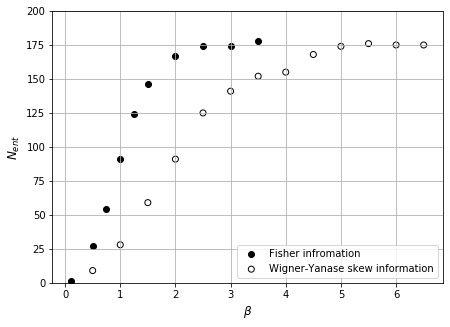
\includegraphics[width=0.95\linewidth]{nanopora_entangled_spins_by_temp}
% 	\caption{
% 		Зависимость оценки числа запутанных спинов в системе от обратной температуры $\beta = \frac{\pi \omega_0}{kT}$
% 		в нанопоре.
% 		Черные круги --- результаты полученные на основе квантовой информации Фишера.
% 		Белые круги --- результаты полученные на основе косой информации Вигнера-Янасе.
% 	}
% 	\label{fig:2}
% \end{figure}
%
% \begin{figure}[H]
% 	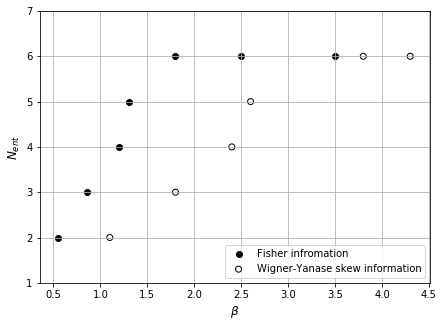
\includegraphics[width=0.95\linewidth]{zigzag_entangled_spins_by_temp}
% 	\caption{
% 		Зависимость оценки числа запутанных спинов  $N_\mathrm{ent}$
% 		от параметра обратной температуры $\beta = \frac{\pi \omega_0}{kT}$
% 		в зигзагообразной цепочке, состоящей из шести спинов.
% 		Черные круги --- результаты полученные на основе квантовой информации Фишера.
% 		Белые круги --- результаты полученные на основе косой информации Вигнера-Янасе.
% 	}
% 	\label{fig:3}
% \end{figure}

\begin{figure}[H]
  \centering
  \begin{subfigure}[t]{0.49\textwidth}
    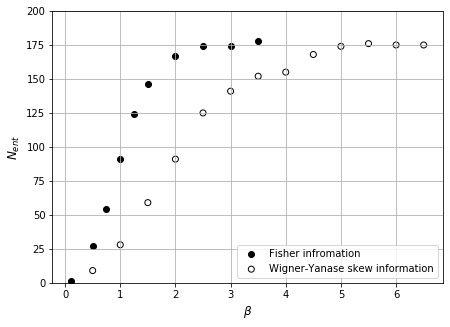
\includegraphics[width=\linewidth]{nanopora_entangled_spins_by_temp}
	\caption{
		Нанопора заполненная спин-несущими частицами.
	}
	\label{fig:qfi-wyi-comparison-nanopora}
  \end{subfigure}
  \hfill
  \begin{subfigure}[t]{0.49\textwidth}
    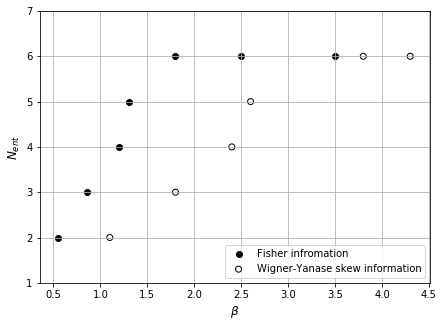
\includegraphics[width=\linewidth]{zigzag_entangled_spins_by_temp}
	\caption{
		Зигзагообразная цепочка, состоящей из шести спинов.
	}
	\label{fig:qfi-wyi-comparison-zigzag-chain}
  \end{subfigure}
  \caption{
    Зависимость оценки снизу числа запутанных спинов  $N_\mathrm{ent}$
	от параметра обратной температуры $\beta = \frac{\pi \omega_0}{kT}$
	Черные круги --- результаты полученные на основе квантовой информации Фишера.
	Белые круги --- результаты полученные на основе косой информации Вигнера-Янасе.
  }
  \label{fig:qfi-wyi-comparison}
\end{figure}

Величины квантовой информации Фишера~$I_\mathrm{F}(\rho(\tau,\beta),I_z)$ и косой информации Вигнера-Яанасе~$I_{WY}(\rho(\tau,\beta),I_z)$
связаны с количеством запутанных частиц в системе (см. раздел~\ref{sec:manyparticle-entanglement-criteria}).
Если величина информации превышает значение $mk^2 + (N - mk)^2$,
где $k, m$ целые числа и $m$ --- это целая часть $N/k$,
тогда гарантируется,
что в системе как минимум $k+1$ частиц связаны в одно несепарабельное состояние.

В разделе~\ref{sec:qfi-wyi-comparison} было получено следующее неравенство
для квантовой информации Фишера и косой информации Вигнера-Янасе:
%
\begin{equation} \label{eq:qfi-wyi-inequality}
    I_{WY}\left(\rho(\tau,\beta), I_z\right)
    \leq I_F\left(\rho(\tau,\beta), I_z\right)
    \leq 2I_{WY}\left(\rho(\tau,\beta), I_z\right).
\end{equation}
%
Неравенство~(\ref{eq:qfi-wyi-inequality}) позволяет надеяться,
что полученные результаты для оценки числа запутанных спинов не будут значительно отличаться.

На Рис.~\ref{fig:qfi-wyi-comparison} представлены результаты зависимости
оценки снизу количества запутанных частиц в системе от обратной температуры $\beta$.
Оценки количества запутанных частиц были полученных на основе квантовой информации Фишера и косой информации Вигнера-Янасе.
Величины обеих информаций были вычислены через второй момент распределения МК когерентностей ЯМР~(cм.
разделы~\ref{sec:reduced-mq-coherences}~и~\ref{sec:wyi-mesuarement}).
На Рис.~\ref{fig:qfi-wyi-comparison-nanopora} сравнение проведено для модели несферической нанопоры,
заполненной газом спин-несущих атомов (например, ксеноном) или молекул в сильном внешнем магнитном поле~(см. раздел~\ref{sec:model-equivalent-spins}).
Расчеты второго момента $M_2(\tau, \beta)$ были сделаны по аналогии с разделом~\ref{sec:nanopora-thermodynamic-equilibrium} для системы из 201 спина.
На Рис.~\ref{fig:qfi-wyi-comparison-zigzag-chain} сравнение проведено
для модели зигзагообразной цепочки ядерных спинов в кристалле гамбергита~(см. раздел~\ref{sec:model-zigzag-chain}).
Расчеты второго момента $M_2(\tau, \beta)$ были сделаны по аналогии с главой~\ref{chapter:manayparticle-entantlement-in-zigzag-chain}

% \section{Обобщения косой информации}
% \begin{align}
%     I_{WY}\left( \rho(t, T), I_z \right) & = 2\sum\limits_k k^2 J_k(t, 2T) = 2M_2(t, 2T) \\
%     I_{WYG}\left( \rho(t, T), I_z \right) &  = -2 \tr{\left[\rho(t, T), I_z\right]} = 2M_2(t, T) \\
%     I_{WYD} \left( \rho(t, T), I_z \right) &  = -2 \mathrm{Tr} \left\{
%         \left[\rho^\alpha, I_z \right] \left[\rho^{1 - \alpha}, I_z \right]
%     \right\}
% \end{align}

\section{Выводы}
Косая информация Вигнера-Янасе, так же как и информация Фишера,
является одной из важнейших мер в теории квантовой информации.
Полученный в этом разделе результат открывает множество возможностей
экспериментального исследования косой информации в различных системах.
В частности, она может быть применена для экспериментального исследования многочастичной запутанности.
Подобные исследования многочастичной запутанности требуют крайне низких температур $<10^{-3}$~K.
В этом случае информация Вигнера-Янасе имеет существенное преимущество перед информацией Фишера,
так как измерение первой для системы с температурой $T$
может быть проведено на установке с вдвое большей температурой $2T$.

% \section{Многоквантовая динамика при низких температурах}
% \input{results/mq-dynamic-at-low-temperature}
%
% \section{Многоспиновая запутанность в системе эквивалентных спинов}
% \input{models/equivalent-spins}
% \input{results/equivalent-spins-entanglement-with-term-equilibrium-state}
% \input{results/equivalent-spins-entanglement-with-dipolar-ordered-state}
%
% \section{Многоспиновая запутанность в цепочках}
% \input{models/zigzag-spin-chain}
% \input{results/zigzag-spin-chain-entanglement}
%
% \section{Определение информации Вигнера-Янасе в МК эксперименте ЯМР}
% \input{results/determination-of-wigner-yanase-information}
%
% \section{Сравнение информации Вигнера-Янасе и Фишера}
% \input{results/comparison-wyi-and-fi}

\section{Итоги}
\chapter*{Заключение}
\addcontentsline{toc}{chapter}{Заключение}

% \input{suplemental-materials}

\end{document}
% \chapter{Измерение квантовой информации Фишера в МК эксперименте ЯМР}
\chapter{Измерение информации Фишера в МК эксперименте ЯМР}
\label{chapter:quantum-fisher-information-measurement}
% (PRA-2019)
% - Расчет динамики при низкой температуре
% - Вычисление второго момента

В разделе~\ref{sec:quantum-fisher-information-mesuarement-at-high-temperature}
была обсуждена связь между вторым моментом распределения интенсивностей МК когерентностей ЯМР и квантовой информацией Фишера~\cite{Toth2014,Pezze2018}.
В частности, было показано,
что в классическом эксперименте ЯМР, когда сигнал усредняется по наблюдаемой $I_z$, в области высоких температур второй момент МК спектра соответствует нижней границе квантовой информации Фишера~\cite{Garttner2018}.
Ниже будет показано, что МК эксперимент ЯМР может быть проведен таким образом,
что связь квантовой информации Фишера и второго момента сохранится для произвольных температур.


\section{МК динамика ЯМР при низких температурах}
%\section{МК когерентности ЯМР}
\begin{figure}[H]
  \centering
  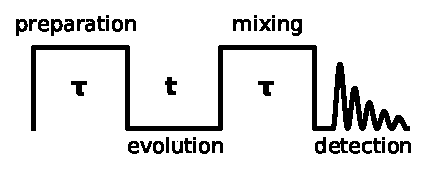
\includegraphics[width=0.5\textwidth]{mq-experiment-schema.pdf}
  \caption{Схема МК эксперимента ЯМР}
  \label{fig:mq-experiment-schema}
\end{figure}

Первоочередно рассмотрим теорию МК динамики ЯМР (см. раздел~\ref{sec:mq-nrm-experiment})
для термодинамически равновесного начального состояния системы $\rho_\mathrm{eq}$,
которое определяется выражением
%
\begin{equation}
  \label{eq:rho_eq}
  \rho_{\mathrm{eq}} = \dfrac{e^{\frac{\hbar\omega_{0}}{kT} I_z}}{Z},
\end{equation}
%
где $Z =\mathrm{Tr}\left\{e^{\frac{\hbar\omega_{0}}{kT} I_z}\right\}$ это статистическая сумма,
$\hbar$ и $k$ --- это постоянная Планка и постоянная Больцмана,
$\omega_0$ --- Ларморовская частота,
$T$ --- температура,
и $I_z$ это оператор проекции полного углового момента на ось $z$,
которая направлена вдоль сильного внешнего магнитного поля.

Для теоретического исследования МК динамики ЯМР
необходимо найти эволюционную матрицу плотности $\rho(\tau)$
на подготовительном периоде МК эксперимента ЯМР (см. раздел~\ref{sec:mq-nrm-experiment}),
решив уравнение Лиувилля~\cite{Feldman2012}
%
\begin{equation}
    \label{eq:liouvile}
    i \dfrac{d\rho(\tau)}{d \tau} =
    \left[H_\mathrm{MQ}, \rho(\tau)\right].
\end{equation}
%
с начальной матрицей плотности $\rho(0)$,
находящейся в термодинамическом равновесии,
%
\begin{equation}
    \label{eq:rho_init}
    \rho(0) = \rho_{\mathrm{eq}}.
\end{equation}
%
Так как в рассматриваемом случае гамильтониан~$H_\mathrm{MQ}$
не зависит от времени,
эволюционная матрица плотности может быть выражена как
\begin{equation}
  \label{eq:rho_eval_lt}
  \rho_\mathrm{LT} (\tau) = e^{-iH_\mathrm{MQ}\tau} \rho_\mathrm{eq} e^{iH_\mathrm{MQ}\tau},
\end{equation}
В области высоких температур,
когда $b = \frac{\hbar\omega_{0}}{kT} \ll 1$,
начальную матрицу плотности $\rho_{\mathrm{eq}}$ можно разложить в ряд по $b$:
%
\begin{equation}
  \label{eq:rho_ht}
  \rho_{\mathrm{eq}} \approx \dfrac{1}{2^N} (1 + bI_z).
\end{equation}
%
В этом случае эволюционную матрицу плотности можно переписать, как
\begin{equation}\label{eq:rho_eval_ht}
  \rho_\mathrm{HT} (\tau) =  e^{-iH_\mathrm{MQ}\tau} I_z e^{iH_\mathrm{MQ}\tau},
\end{equation}

Экспериментальное исследование МК динамики ЯМР заключается в проведении
МК эксперимента ЯМР (см. раздел~\ref{sec:mq-nrm-experiment})
и последующем измерении интенсивностей МК когерентностей ЯМР.
В результате проведения всех периодов МК эксперимента ЯМР (Рис.~\ref{fig:mq-experiment-schema})
итоговый сигнал $G(\tau, \phi)$ хранится в информации о населенности\cite{Feldman1997}.
Выражение для сигнала $G(\tau, \phi)$ имеет вид
%
\begin{equation}
  \label{eq:signal}
   G(\tau, \phi)
   = \tr{
     e^{iH_\mathrm{MQ}\tau} e^{i\phi I_z} e^{-iH_\mathrm{MQ}\tau}
     \rho_\mathrm{eq}
     e^{iH_\mathrm{MQ}\tau} e^{-i\phi I_z} e^{-iH_\mathrm{MQ}\tau}
     I_z
    }.
\end{equation}
%
Перегруппировкой множителей,
выражение~(\ref{eq:signal}) может быть переписано через
 $\rho_\mathrm{LT} (\tau)$ и $\rho_\mathrm{HT} (\tau)$:
%
\begin{equation}
  \label{eq:signal-short}
  G(\tau, \phi) = \tr{
   e^{i\phi I_z} \rho_\mathrm{LT} (\tau)
   e^{-i\phi I_z} \rho_\mathrm{HT} (\tau).
  }
\end{equation}


Для получения выражений сигналов отдельных когерентностей,
перейдем к представлению матриц плотности
$\rho_\mathrm{LT} (\tau)$ и $\rho_\mathrm{HT} (\tau)$
в виде ряда
%
\begin{equation}\label{eq:rho_series}
  \rho_\mathrm{LT} (\tau) = \sum_n \rho_{LT, n}(\tau); \quad
  \rho_\mathrm{HT} (\tau) = \sum_n \rho_{HT, n}(\tau),
\end{equation}
%
где $\rho_{LT, n} (\tau)$ и  $\rho_{HT, n} (\tau)$
это вклад МК когерентности $n$-ого порядка
в матрицы плотности $\rho_\mathrm{LT} (\tau)$ и $\rho_\mathrm{HT} (\tau)$ соответственно.
Подставляя~(\ref{eq:rho_series}) в~(\ref{eq:signal}) итоговый сигнал $G(\tau, \phi)$ МК когерентностей ЯМР можно переписать как
%
\begin{equation}
    \label{eq:signal_series}
    G(\tau, \phi) = \sum\limits_n
    e^{in\phi}\mathrm{Tr} \left\{
    \rho_{LT, n}(\tau) \rho_{HT, -n} (\tau)
    \right\},
\end{equation}
%
где учтены коммутационные соотношения
%
\begin{equation}
    \left[I_z, \rho_{LT, n} (\tau) \right] = n  \rho_{LT, n} (\tau);
    \quad
    \left[I_z, \rho_{HT, n} (\tau) \right] = n  \rho_{HT, n} (\tau).
\end{equation}

Нормированные интенсивности МК когерентностей ЯМР могут быть выражены следующим образом
%
\begin{equation}
    \label{eq:coherence}
    J_n(\tau)
    = \dfrac{
       \mathrm{Tr} \left\{
        \rho_{LT, n}(\tau) \rho_{HT, -n} (\tau)
        \right\}
    }{Tr \left\{\rho_{\mathrm{eq}}I_z\right\}}.
    = \dfrac{
       \mathrm{Tr} \left\{
        \rho_{LT, n}(\tau) \rho_{HT, -n} (\tau)
        \right\}
    }{\frac N 2 \tanh \frac b 2}.
\end{equation}

МК когерентности ЯМР имеют несколько свойств.
Во-первых, в момент времени  $\tau=0$
нормированная интенсивность $J_0(0)$ МК когерентности ЯМР нулевого порядка равна 1,
а остальные интенсивности равны нулю.
Во-вторых, сумма всех нормированных когерентностей равна единице.
Докажем это утверждение.
Используя выражения~(\ref{eq:rho_eq}) и~(\ref{eq:rho_eval_ht})
выразим $\rho_\mathrm{LT}(\tau)$ через $\rho_\mathrm{HT}(\tau)$.
%
\begin{equation}\label{eq:lt-through-ht}
  \rho_\mathrm{LT}(\tau) = \dfrac 1 Z
  \exp\left(be^{-iH_\mathrm{MQ}\tau} I_z e^{iH_\mathrm{MQ}\tau}\right) =
  \dfrac 1 Z e^{b\rho_\mathrm{HT}(\tau)}.
\end{equation}
%
Подставляя выражение~(\ref{eq:lt-through-ht}) в~(\ref{eq:coherence}) получаем
%
\begin{multline}
  \label{eq:sum_of_coherence}
  \sum\limits_n J_n(\tau) =
  \dfrac{\sum\limits_{n, m}\mathrm{Tr}\left\{
      \rho_{LT, n}(\tau)\rho_{HT, m}(\tau)
  \right\}}
  {\mathrm{Tr}\left\{\rho_\mathrm{eq} I_z\right\}} = \\
  \dfrac{\mathrm{Tr}\left\{
      \rho_\mathrm{LT}(\tau)\rho_\mathrm{HT}(\tau)
  \right\}}
  {\mathrm{Tr}\left\{\rho_\mathrm{eq} I_z\right\}} =
  \dfrac{\mathrm{Tr}\left\{
      \rho_\mathrm{HT}(\tau)e^{b\rho_\mathrm{HT}(\tau)}
  \right\}}
  {Z\mathrm{Tr}\left\{\rho_\mathrm{eq} I_z\right\}} = \\
  \dfrac{\frac{d}{db} \ln \mathrm{Tr}\left\{
      e^{b I_z}
  \right\}}
  {\mathrm{Tr}\left\{\rho_\mathrm{eq} I_z\right\}} =
  \dfrac{\frac 1 2 N \tanh \left( \frac b 2 \right)}
  {\frac 1 2 N \tanh \left( \frac b 2 \right)} = 1.
\end{multline}
Ур.~(\ref{eq:sum_of_coherence}) подтверждает,
что сумма МК когерентностей ЯМР сохраняется на подготовительном периоде МК эксперимента ЯМР.


\section{Приведенные МК когерентности ЯМР}
\label{sec:reduced-mq-coherences}

В предыдущем разделе было получено выражение~(\ref{eq:signal-short}) коррелятора сигнала $G(\tau, \phi)$,
которое в области высоких температур имеет вид
%
\begin{equation}
    \label{eq:otoc-ht}
    G_\mathrm{HT}(\tau, \phi) = \frac b Z\mathrm{Tr}\left\{
    e^{i \phi I_z}
    \rho_\mathrm{HT} (\tau)
    e^{-i \phi I_z}
    \rho_\mathrm{HT}(\tau)
    \right\},
\end{equation}
%
так как согласно разложению~(\ref{eq:rho_ht})
%
\begin{equation}
  \rho_\mathrm{LT} (\tau) \approx \frac 1 Z + \frac b Z \rho_\mathrm{HT}.
\end{equation}
%
Так же в разделе~\ref{sec:quantum-fisher-information-mesuarement-at-high-temperature}
было отмечено,
что связь второго момента МК спектра ЯМР и квантовой информации Фишера
обеспечивается благодаря особому виду коррелятора сигнала.
% Коррелятор должен принадлежать классу неупорядоченных по времени корреляторов ``out-of-time-ordered correlator'' (OTOC).
Выражение~(\ref{eq:otoc-ht}) для $G_\mathrm{HT}(\tau, \phi)$
в высоко температурной области
удовлетворяет этому требованию,
в отличие от выражения~(\ref{eq:signal-short}) для $G(\tau, \phi)$.
$G(\tau, \phi)$ не является неупорядоченным по времени коррелятором,
так как выражение~(\ref{eq:signal}) содержит разные матрицы $\rho_\mathrm{LT}(\tau)$ и $\rho_\mathrm{HT}(\tau)$.
Однако можно обобщить МК эксперимент ЯМР  таким образом,
чтобы привести сигнал $G(\tau, \phi)$ к нужному виду.
Для достижения такого поведения коррелятора финального сигнала МК эксперимента ЯМР
необходимо усреднить сигнал,
полученный после трех периодов %МК эксперимента ЯМР
(Рис.~\ref{fig:mq-experiment-schema}),
по начальному состоянию $\rho_\mathrm{eq}$.
Тогда коррелятор сигнала будет описываться следующим выражением
%
\begin{multline}
  \label{eq:otoc_LT}
  G_\mathrm{LT}(\tau, \phi) =
  \mathrm{Tr}\left\{
    e^{i H_{\mathrm{MQ}} \tau}
    e^{i \phi I_z}
    e^{-i H_{\mathrm{MQ}} \tau}
    \rho_{\mathrm{eq}}
    e^{i H_{\mathrm{MQ}}}
    e^{-i \phi I_z}
    e^{-i H_{\mathrm{MQ}} \tau}
    \rho_{\mathrm{eq}}
  \right\} \\ =
  \mathrm{Tr}\left\{
    e^{i \phi I_z}
    e^{-i H_\mathrm{MQ} \tau}
    \rho_\mathrm{eq}
    e^{i H_\mathrm{MQ} \tau}
    e^{-i \phi I_z}
    e^{-i H_\mathrm{MQ} \tau}
    \rho_{\mathrm{eq}}
    e^{i H_\mathrm{MQ} \tau}
  \right\} \\ =
  \mathrm{Tr}\left\{
    e^{i \phi I_z}
    \rho_\mathrm{LT} (\tau)
    e^{-i \phi I_z}
    \rho_\mathrm{LT} (\tau)
  \right\}.
\end{multline}
%
Из выражения~(\ref{eq:otoc_LT}) следует,
что $G_\mathrm{LT}(\tau, \phi)$ является неупорядоченным по времени коррелятором при произвольных температурах.
Важно отметить,
что полученный результат для начальной матрицы~(\ref{eq:rho_eq}) легко обобщить
на произвольное начальное состояние.
Связь квантовой информации Фишера и второго момента будет выполняться всегда,
если по итогу трех периодов (Рис.~\ref{fig:mq-experiment-schema}) МК экскремента ЯМР
проводить усреднение по начальному состоянию.
Это наблюдение будет играть важную роль в следующей Главе~\ref{chapter:manyparticle-entanglement-in-nanopore}
при рассмотрении МК динамики ЯМР дипольных упорядоченных состояний.

Нормированные интенсивности МК когерентностей ЯМР для сигнала $G_\mathrm{LT}(\tau, \phi)$
могут быть записаны по аналогии с~(\ref{eq:coherence}):
%
\begin{equation}\label{eq:reduced-mq-coherences}
    J_{\mathrm{LT}, n}(\tau) =
    \frac{\mathrm{Tr} \left\{
        \rho_{\mathrm{LT},n}(\tau)
        \rho_{\mathrm{LT}, -n}(\tau)
    \right\}}
    {\mathrm{Tr}\left\{\rho^2_\mathrm{eq}\right\}}.
\end{equation}
%
В этом случае нормировочный член определяется как
%
\begin{equation}\label{eq:j_lt_norm}
  \mathrm{Tr}\left\{\rho^2_\mathrm{eq}\right\} =
    \frac{2^N \cosh^N(b)}{Z^2}.
\end{equation}
Когерентности определяемые выражением~(\ref{eq:reduced-mq-coherences})
являются приведенными МК когерентностями ЯМР.
%
Используя разложение~(\ref{eq:rho_series}),
сумма интенсивностей приведенных МК когерентностей ЯМР~(\ref{eq:reduced-mq-coherences}) может быть записана как
%
\begin{multline}\label{eq:reduced-coherences-sum}
  \sum\limits_{n} J_{\mathrm{LT}, n}(\tau)
  = \dfrac{
    \tr{
      \sum\limits_{n}
      \rho_{\mathrm{LT}, n}(\tau)
      \rho_{\mathrm{LT},-n}(\tau)}
    }{
    \tr{\rho^2_\mathrm{eq} }
  }
  = \dfrac{
    \tr{
      \sum\limits_{m,n}
      \rho_{\mathrm{LT}, n}(\tau)
      \rho_{\mathrm{LT}, m}(\tau)
    }}{
    \tr{\rho^2_\mathrm{eq}}
  }
  \\
  = \dfrac{
    \tr{\rho_\mathrm{LT}^2(\tau)}
  }{
    \tr{\rho^2_\mathrm{eq}(\tau)}
  }
  = \dfrac{
    \tr{
      e^{-i H_\mathrm{MQ} \tau}
      \rho^{2}_\mathrm{eq}
      e^{i H_\mathrm{MQ} \tau}
    }
  }{
    \tr{ \rho^2_\mathrm{eq}}
  }
  = 1.
\end{multline}
%
Из уравнения~(\ref{eq:reduced-coherences-sum}) можно сделать вывод, что сумма МК~когерентностей~ЯМР~сохраняется на подготовительном периоде МК~эксперимента~ЯМР~\cite{Baum1985}.


Удвоенный второй момент (дисперсия) $M_2(\tau)$ распределения интенсивностей приведенных МК когерентностей ЯМР $J_{\mathrm{LT}, n} (\tau)$
является нижней границей квантовой информации Фишера $F_{Q}$
(см. раздел~\ref{sec:quantum-fisher-information-mesuarement-at-high-temperature}):
\begin{equation}\label{eq:fisher-low-bound}
  F_{Q}(\tau) \geq 2M_2(\tau),
\end{equation}
где второй момент может быть выражен~\cite{Khitrin1997} как
%
\begin{equation}\label{eq:m2-via-coherences}
  M_2(\tau) = \sum\limits_n n^2 J_{\mathrm{LT}, n} (\tau).
\end{equation}

\section{Выводы}
В этой главе было предложено обобщение МК эксперимента ЯМР,
позволяющее измерять нижнюю границу квантовой информации Фишера
в произвольный момент времени подготовительного периода МК эксперимента ЯМР
с произвольным начальным состоянием системы.
В свою очередь квантовая информация Фишера является ключевой концепцией в квантовой теории информации
и основной мерой в квантовой метрологии.
В частности квантовая информация Фишера может выступать в качестве количественной оценки запутанных частиц в системе.
Таким образом, становится возможным исследование многочастичной запутанности в МК эксперименте ЯМР.
Более того, разработанный подход позволяет исследовать температурную зависимость многочастичной запутанности.

% При высоких температурах интенсивность МК когерентностей ЯМР может быть исследована экспериментально с помощью обычных МК экспериментов ЯМР.
Результаты полуаналитического анализа многочастичной запутанности в системе спин-несущих молекул (атомов) представлены в следующей главе~\ref{chapter:manyparticle-entanglement-in-nanopore}.
% \subsection{Создание дипольно упорядоченных состояний}
% (PRA-2019) 
%   - Температурная зависимость многочастичной запутанности 
%   - Зависимость от числа частиц 
% 
% Многоспиновая запутанность c дипольно упорядоченном начальном

% JETP-2020
% \chapter{Многоспиновая запутанность в зигзагообразной цепочке}
\chapter{Многоспиновая запутанность в квазиодномерных цепочках}
\label{chapter:manayparticle-entantlement-in-zigzag-chain}

В предыдущей главе~\ref{chapter:manyparticle-entanglement-in-nanopore}
была подробно исследована многочастичная запутанность,
возникающая в МК эксперименте ЯМР в нанопоре.
Данная модель показала себя отличной площадкой
для исследования запутанности многих взаимодействующих частиц.
Тем не менее одномерные модели значительно лучше изучены как теоретически,
так и экспериментально~(см. раздел~\ref{sec:model-uniform-chain}).
В этой главе будет исследована многочастичная запутанность,  возникающая в таких системах. Основные результаты этой главы отражены в работах G.A. Bochkin, E.B. Fel'dman, E.I. Kuznetsova, I.D. Lazarev, S.G. Vasil'ev, V.I. Volkov, 1H NMR in a quasi-one-dimensional zig-zag spin chain of hambergite, Be2BO3(OH), \textit{Journal of Magnetic Resonance}, 319:106816, 2020
и
G. A. Bochkin, S. I. Doronin, E. I. Kuznetsova, I. D. Lazarev, E. B. Fel'dman, S. G. Vasil'ev, Many-Spin Entanglement in Zigzag Spin Chain in Multiple Quantum NMR, \textit{Applied Magnetic Resonance}, 51(7):667-678, 2020.



\section{Однородная цепочка}
Однородная цепочка является наиболее простой разновидностью одномерной системы.
Создание запутанных кластеров в таких цепочках ограничено слабыми ДДВ удаленных спинов.
В МК эксперименте ЯМР в однородной цепочке существенны когерентности только нулевого и плюс/минус второго порядков.
Оценка снизу информации Фишера может быть получена с помощью Гауссова приближения для распределения интенсивностей МК когерентностей~\cite{Baum1985}.
В этом случае выражение для МК когерентностей имеет
%
\begin{equation}\label{eq:gaussaprox}
  J(\tau, T)=\dfrac{1}{\sqrt{\pi N_c(T)}} \exp\p{-\frac{n^2}{N_c(T)}},
\end{equation}
%
где $N_c(T)$ -- число коррелированных спинов,
ответственных за создание профиля МК когерентности.
Поскольку удвоенный второй момент интенсивностей МК когерентностей $2M_2(\tau, T)$ является нижней границей квантовой информации Фишера $F_Q$
(см.~раздел~\ref{sec:quantum-fisher-information-mesuarement-at-high-temperature}),
из уравнения~(\ref{eq:gaussaprox}) можно найти, что
%
\begin{equation}\label{eq:qfisheinf}
  F_Q \geq 2M_2(\tau, T) = N_c(T) \geq N,
\end{equation}
%
где $N$ --- число узлов в цепочке.
Для небольших значений $k$ верхнюю границу информации Фишера $k$-сепарабельного состояния
$F^k_Q = \sup{F_Q\p{\rho_{k-\mathrm{prod}}}}$~(см.~раздел.~\ref{sec:manyparticle-entanglement-criteria}) можно переписать в приближённой форме как
%
\begin{equation}\label{eq:inequalityforfq2}
  F^k_Q \leq k N.
\end{equation}
%
Неравенство~(\ref{eq:inequalityforfq2}) не нарушается ни для какого $k > 0$, когда $F_Q = N$,
а для случая $F_Q > N$ детектируется только парная запутанность.
Полученная оценка согласуется с представленными в литературе~\cite{Doronin2007, Feldman2012} результатами.

Из выражения~(\ref{eq:qfisheinf}) также следует,
что увеличение числа узлов цепочки не способствует детектированию запутанных кластеров большего размера, чем двухчастичный.
Тем не менее этого достаточно для передачи МК когерентностей вдоль цепочки~\cite{Bochkin2018qip} и создания запутанности между удаленными концами цепочки~\cite{Lazarev2019}.

% \subsection{Температурная зависимость запутанности удаленных узлов цепочки}
\subsection{Запутанность удаленных узлов цепочки}
\label{subsec:entanglement-of-remote-chain-nodes}
Однородная цепочка является удобной моделью линии связи для передачи квантовых состояний на короткие расстояния.
Типичная схема линии связи (см.~Рис.\ref{fig:model-uchain-schema}) состоит из передатчика (sender $S$),
приемника (reciever $R$)
и линии передачи (transmition line $TL$).
Также ряд протоколов передачи задействуют расширенный приемник (extended reciever $ER$),
на котором применяется специально сконструированное универсальное унитарное преобразование для наилучшего восстановления передаваемой информации~\cite{Feldman2021}.

\begin{figure}[H]
  \centering
  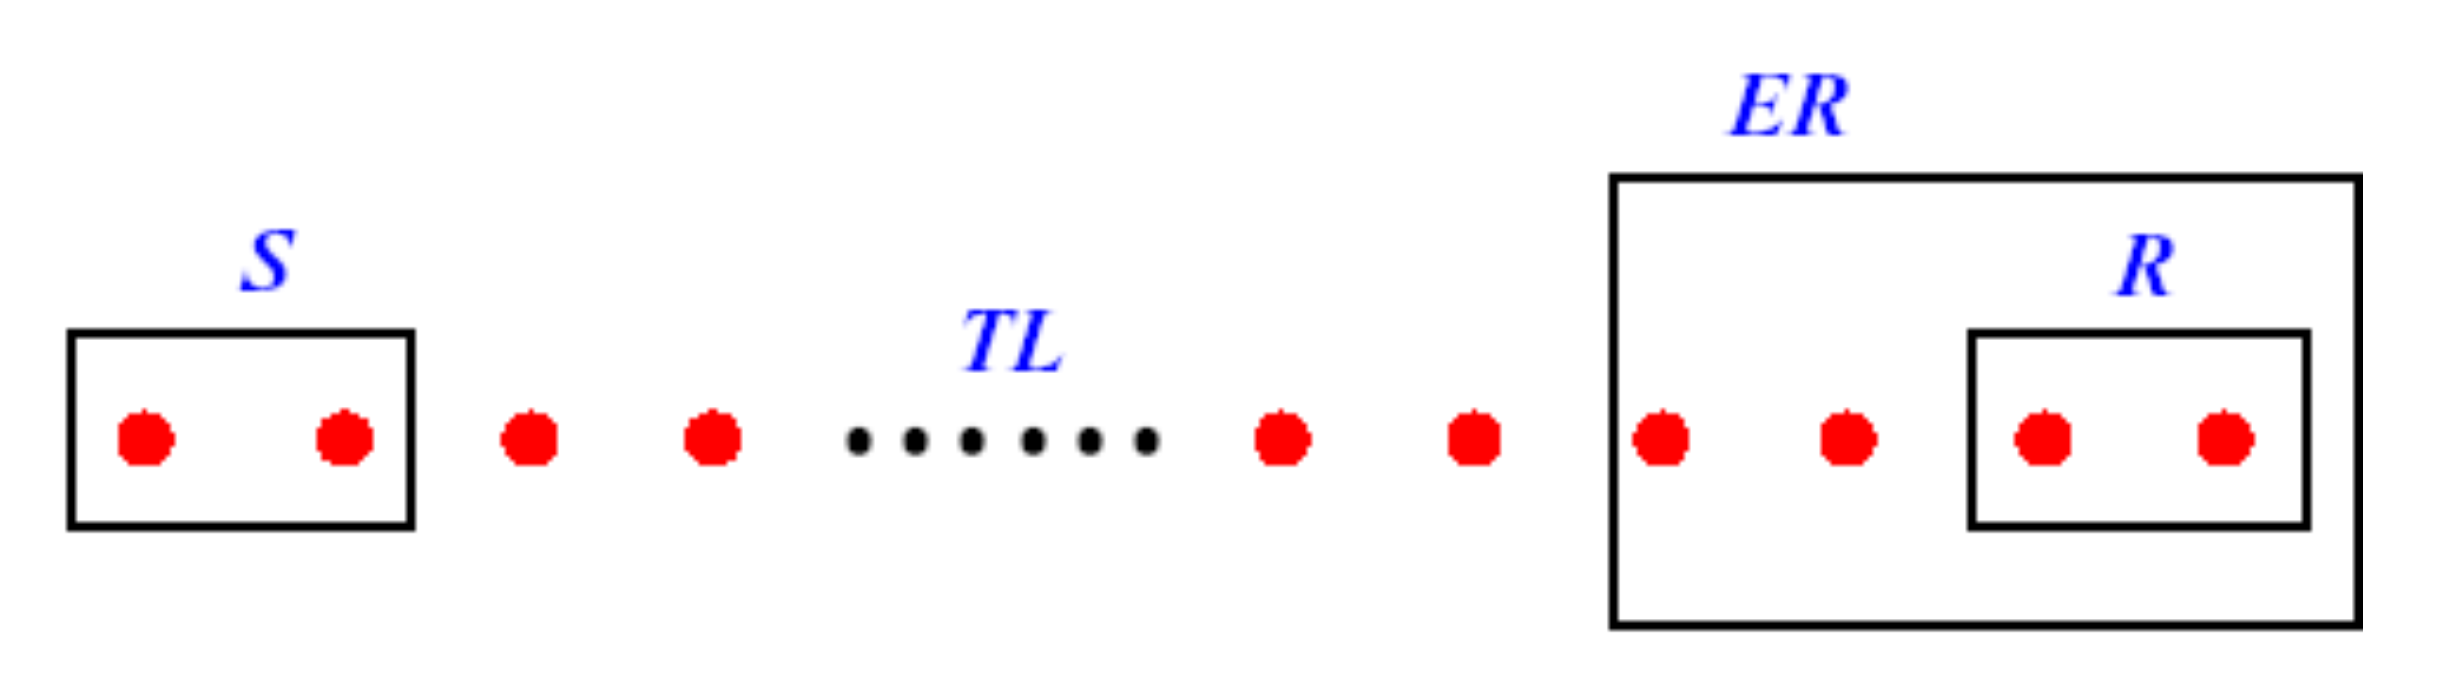
\includegraphics[width=0.9\textwidth]{model-uchain-schema.png}
  \caption{
    Схематичное изображение линии передачи квантовых состояний.
    S --- передатчик,
    TL --- линия передачи,
    ER --- расширенный приемник,
    R --- приемник.
  }
  \label{fig:model-uchain-schema}
\end{figure}

В оригинальной работе Бозе~\cite{Bose2003} был рассмотрен случай передачи однокубитного состояния под действием гейзенберговского гамильтониана.
В рамках МК спектроскопии ЯМР более естественно рассматривать передачу под действием $XX$-гамильтониана,
который для однородной цепочки совпадает с МК гамильтонианом $\hmq$~(\ref{eq:hmq}) с точностью до поворота~(см.~раздел~\ref{sec:model-uniform-chain}).
В приближении ближайших соседей во вращающейся системе координат с Ларморовской частотой $\omega_0$ выражение $XX$-гамильтониана имеет вид:
%
\begin{equation}\label{eq:hxx}
  H_\mathrm{XX} = D\sum_{j=1}^{N-1}\p{I_{j,x}I_{j+1,x} + I_{j,y}I_{j+1,y}},
\end{equation}
где $D$ --- константна ДДВ между соседними узлами,
а N --- число узлов в цепочке.
В базисе бесспиновых фермионных операторов $\gamma_j$ and $\gamma_j ^+$
гамильтониан~(\ref{eq:hxx}) имеет диагональный вид
\begin{equation}\label{Diagonal_Hamiltonian}
  H_\mathrm{XX}=\sum\limits _{k}\varepsilon _{k}\gamma ^{+}_{k}\gamma _{k}.
\end{equation}
Переход к новому базису определяется преобразованием Йордана-Вигнера~\cite{Jordan1928, Feldman1998}:
\begin{equation}\label{eq:jw_operators}
  \gamma _{k}=\sum\limits ^{N}_{j=1}g_{kj} c_{j},
  \quad
  \gamma^+ _{k}=\sum\limits ^{N}_{j=1}g_{kj} c_{j}^+,
\end{equation}
где операторы рождения/уничтожения
\begin{equation}\label{eq:creation_annihilation_operators}
  c_{j}=(-2)^{j-1}I_{1,z}I_{2,z}I_{3,z}...I_{j-1,z}I^-_j,
  \quad
  c_{j}^+=(-2)^{j-1}I_{1,z}I_{2,z}I_{3,z}...I_{j-1,z}I^+_j,
\end{equation}
и
\begin{equation}\label{eq:gammakj}
  \varepsilon_{k} = D \cos(k),
  \quad
  g_{kj} =\sqrt {\frac {2}{N+1}}\sin \left( kj\right),
  \quad
  k=\frac {\pi n}{N+1}\quad n=1\ldots N .
\end{equation}

В общем случае в начальный момент времени однокубитный передатчик --- это произвольное чистое состояние
%
\begin{equation}\label{eq:random-pure-state}
  \ket{\psi_\mathrm{init}} = a\ket{0} + b\ket{1},
  \quad
  |a|^2 + |b|^2 = 1,
\end{equation}
%
а линия передачи и приемник находятся в термодинамическом равновесном состоянии
%
\begin{equation}
    \rho^\mathrm{TL, R}_\mathrm{init} = \otimes_{i=2}^N e^{\beta I_{i, z}}.
\end{equation}

Эволюционная матрица плотности может быть найдена из стационарного уравнения Лиювилля
\begin{equation}\label{eq:eval-rho-liuville}
  \rho(t) = e^{-iH_\mathrm{XX}t}
    \ket{\psi_\mathrm{init}} \bra{\psi_\mathrm{init}}
    \otimes
    \rho^\mathrm{TL, R}_\mathrm{init}
    e^{iH_\mathrm{XX}t}.
\end{equation}
После проведения редукции эволюционной матрицы плотности $\rho(t)$~(\ref{eq:eval-rho-liuville}),
матрица плотности передатчика и приемника определяется выражением
%
\small
\begin{equation}\label{eq:eval-rho-sr}
\rho^\mathrm{S,R}(t) =
\begin{pmatrix}
  \begin{array}{r}
    L(|f|^2+|g|^2) \\
    + \frac{e^{2\beta}}{(e^{\beta}+1)^2}
  \end{array}
  &
  \begin{array}{r}
    -\p{-\tanh\frac{\beta}{2}}^{N-2} \\
    \times \frac{ab^*f^* e^{\frac{\beta}{2}}}{2\cosh\frac{\beta}{2}}
  \end{array}
  &
  \frac{ab^* e^{\beta /2}}{2\cosh\frac{\beta}{2}}g^*
  &
  0\\
  &
  &
  &\\
  \begin{array}{r}
    -\p{-\tanh\frac{\beta}{2}}^{N-2} \\
    \times\frac{a^*bf e^{\frac{\beta}{2}}}{2\cosh\frac{\beta}{2}}
  \end{array}
  &
  \begin{array}{r}
    L(e^{-\beta}|g|^2-|f|^2) \\
    +\frac{1}{2\cosh{\beta}+2}
  \end{array}
  &
  \begin{array}{r}
    {2\p{-\tanh\frac{\beta}{2}}^{n-2}}\\
    \times Lfg^*\cosh\frac{\beta}{2}
  \end{array}
  &
  \frac{ab^* e^{-\beta/2}}{2\cosh\frac{\beta}{2}}g^* \\
  &
  &
  &\\
  \frac{a^*b e^{\beta /2}}{2\cosh\frac{\beta}{2}}g
  &
  \begin{array}{r}
   2\p{-\tanh\frac{\beta}{2}}^{n-2}\\ \times{Lf^*g\cosh\frac{\beta}{2}}
  \end{array}
  &
  \begin{array}{r}
    L(e^{-\beta}|f|^2 -|g|^2) \\
    +\frac{1}{2\cosh{\beta}+2}
  \end{array}
  &
  \begin{array}{r}
    \p{-\tanh\frac{\beta}{2}}^{N-2} \\
    \times \frac{ab^*f^* e^{-\frac{\beta}{2}}}{2\cosh\frac{\beta}{2}}
  \end{array}
  &
  &
  &\\
  0
  &
  \frac{a^*b e^{-\beta /2}}{2\cosh\frac{\beta}{2}}g
  &
  \begin{array}{r}
    \p{-\tanh\frac{\beta}{2}} ^{N-2} \\
    \times \frac{a^*bf e^{-\frac{\beta}{2}}}{2\cosh\frac{\beta}{2}}
  \end{array}
  &
  \begin{array}{r}
    -L e^{-\beta}(|f|^2 +|g|^2)\\
    + \frac{1}{(e^{\beta}+1)^2}
  \end{array}
\end{pmatrix},
\end{equation}
\normalsize
где $f={f_N(t, N)}$, $g={f_N(t, 1)}$, $L=\frac{1-2|b|^2 e^{\frac{\beta}{2}}\cosh\frac{\beta}{2}}{\cosh\frac{\beta}{2}}$
и
%
\begin{equation}
  f_N(t, j) = \frac{2}{N+1}\sum_k e^{i\epsilon_k t}\sin k \sin jk.
\end{equation}

\begin{figure}[H]
  \begin{subfigure}{0.45\textwidth}
    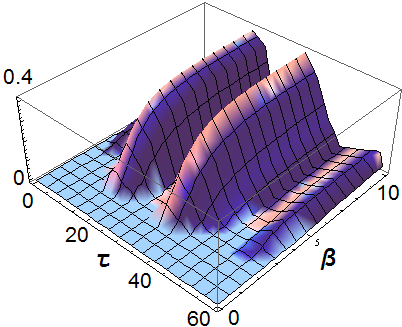
\includegraphics[width=\textwidth]{concurence-temp-uniform-chain-N4.png}
    \caption{
      $\ket{\psi} = \dfrac{\ket{0} + \ket{1}}{\sqrt{2}}$
    }
    \label{fig:concurence-temp-uniform-chain-N4}
  \end{subfigure}
  \hfill
  \begin{subfigure}{0.45\textwidth}
    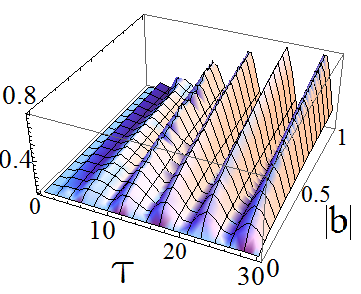
\includegraphics[width=\textwidth]{concurence-polarization-uniform-chain-N4.png}
    \caption{
      $\beta = 5$
    }
    \label{fig:concurence-polarization-uniform-chain-N4}
  \end{subfigure}
  \caption{
    Зависимость согласованности $C$ от безразмерного времени $\tau = Dt$,
    обратной температуры $\beta$
    (cм. Рис.~\ref{fig:concurence-temp-uniform-chain-N4})
    и величины поляризации $|b|$
    (cм. Рис.~\ref{fig:concurence-polarization-uniform-chain-N4})
    при передаче квантового состояния по цепочке из $N=4$ спинов.
  }
  \label{fig:councurence-uniform-chain-N4}
\end{figure}

В качестве критерия запутанности для двухкубитного смешанного состояния удобнее всего использовать критерий Вуттерса~(см. раздел. ~\ref{sec:entanglement-criteria}) на основе согласованности $C$.
Температурная зависимость согласованности $C$ при передаче чистого состояния $\ket{\psi} = \frac{\ket{0} + \ket{1}}{\sqrt{2}}$ ($a=b=\frac{1}{\sqrt{2}}$) представлена на Рис.~\ref{fig:concurence-temp-uniform-chain-N4}.
При обратной температуре $\beta > 1$ приемник и передатчик запутываются.
На Рис.~\ref{fig:concurence-polarization-uniform-chain-N4} представлена зависимость согласованности $C$ от различных значений начальной поляризации передатчика при обратной температуре $\beta = 5$.
Приемник и передатчик запутываются при любой начальной поляризации.

\begin{figure}[H]
    \centering
    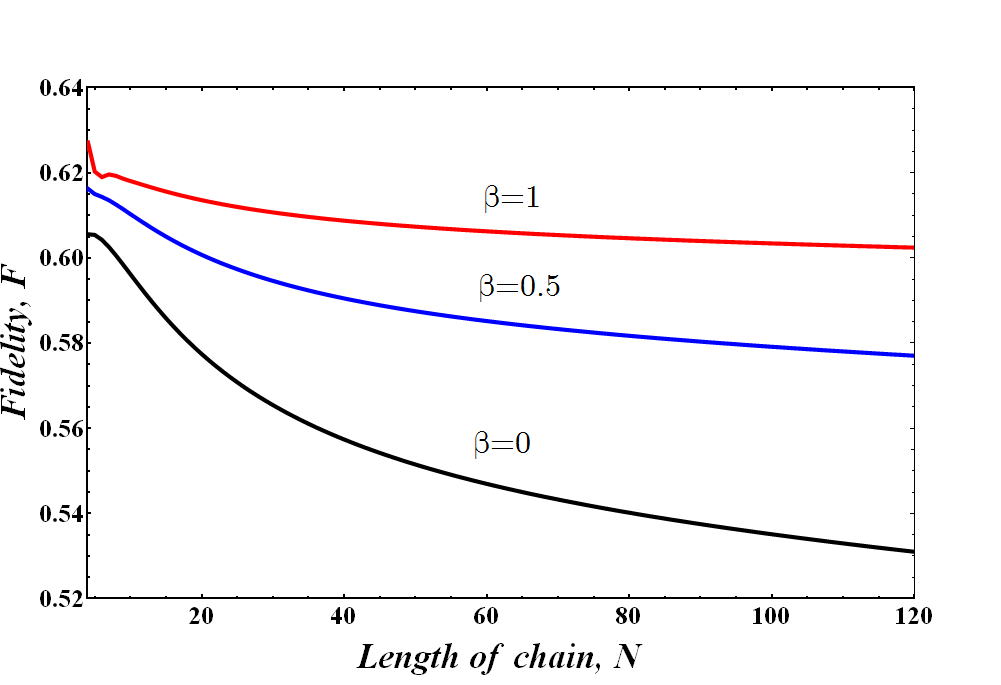
\includegraphics[width=0.8\textwidth]{fidelity-n-beta.png}
    \caption{
      Зависимость фиделити переданного состояния
      $\rho^\mathrm{S}_\mathrm{init}$
      и полученного
      $\rho^\mathrm{R}\p{\bar\tau_N}$
      от количества узлов в цепи.
      Разные линии соответствуют разным значениям обратной температуры $\beta$.
     }
    \label{fig:fidelity-n-beta}
\end{figure}

Идеальная передача произвольного квантового состояния в спиновых цепочках достижима только в очень специфических случаях~\cite{Christandl2004, Karbach2005} и может быть легко разрушена небольшими возмущениями гамильтониана взаимодействия.
В общем случае передача осуществляться не идеально,
но с высокой вероятностью.
Качество передачи можно оценить с помощью фиделити~\cite{Jozsa1994}
%
\begin{equation}\label{generalFidelity}
  F\p{\rho^\mathrm{S}_\mathrm{init}, \rho^\mathrm{R}\p{t}}
  = \tr{\rho^\mathrm{S}_\mathrm{init}, \rho^\mathrm{R}(t)}.
\end{equation}
%
С учетом $\rho^\mathrm{R}\p{t} = \tr{\rho^\mathrm{S,R}(t)}_\mathrm{S}$,
аналитическое выражение для фиделити имеет вид
%
\begin{multline}\label{exactfidelity}
  F\p{\rho^\mathrm{S}_\mathrm{init}, \rho^\mathrm{R}\p{t}}
  = (1-2|b|^2)\p{
    \frac{e^{\beta/2}}{\cosh \beta/2}
    + \p{\frac{e^{-\beta/2}}{\cosh \beta/2} -|b|^2 }
      \left|f_N(t, N)\right|^2
  } \\
  + |b|^2
  + 2 |b|^2 \p{1-|b|^2} \Re\left\{f_N(t, N)\right\}
  \p{-\tanh \p{\frac{\beta}{2}}}^{N-1}.
\end{multline}
%
Время $\bar\tau_{N}$, при котором фиделити достигает первого пика, называется временем передачи~\cite{Feldman2016}.
Оно совпадает с временем первого пика функции $\left|f_N(t, N)\right|^2$.
Фиделити~\cite{Jozsa1994} переданного и полученного квантового состояния в момент времени $\bar\tau_{N}$ уменьшается с увеличением длинны цепочки (см. Рис.\ref{fig:fidelity-n-beta}).


\subsection{Идеальная передача запутанных состояний}
% \subsection{Идеальная передача МК когерентности нулевого порядка}

гамильтониан $H_\mathrm{XX}$ коммутирует с $z$-проекцией $I_z$ полного спинового момента
и сохраняет число возбуждений в процессе эволюции.
В этом случае когерентности разных порядков не перемешиваются~\cite{Feldman2017} и могут быть рассмотрены отдельно~\cite{Bochkin2018qip}.
В частности, было показано~\cite{Feldman2021},
что специальная форма когерентности нулевого порядка может передаваться без потерь
по цепочке из $N$ узлов, находящейся в основном состоянии:
%
\begin{equation}
  \rho^\mathrm{TL}_\mathrm{init} = \otimes^{N_\mathrm{TL}}_{i=1}\ket{0},
  \quad
  \rho^\mathrm{R}_\mathrm{init} = \otimes^{N_\mathrm{R}}_{i=1}\ket{0},
\end{equation}
%
где $N_\mathrm{R}$ --- количество кубитов в приёмнике,
а $N_\mathrm{TL}  = N - 2 N_\mathrm{R}$.
В случае, когда количество кубитов в передатчике $N_\mathrm{S} = N_\mathrm{R} = 3$,
специальная матрица плотности передатчика,
которая может быть передана без потерь,
в базисе с одним возбуждением
$\left \{\ket{000}, \ket{001}, \ket{010}, \ket{100} \right\}$
может быть записана в виде
%
\begin{equation}
  \rho^\mathrm{S}_\mathrm{init} =
  \begin{pmatrix}
    u &    0     &    0    & 0 \\
    0 &   x_1    & \omega  & 0 \\
    0 & \omega^* &   x_2   & 0 \\
    0 &    0     &    0    & v
  \end{pmatrix}.
\end{equation}
%
После редукции $\rho^\mathrm{S}_\mathrm{init}$ по первому спину
матрица плотности оставшихся двух в полном базисе имеет вид
\begin{equation}\label{eq:rho-s-reduced}
  \tr{\rho^\mathrm{S}_\mathrm{init}}_{1} =
  \begin{pmatrix}
    u + v &    0     &    0    & 0 \\
    0     &   x_1    & \omega  & 0 \\
    0     & \omega^* &   x_2   & 0 \\
    0     &    0     &    0    & 0
  \end{pmatrix}.
\end{equation}
Для матрицы вида~(\ref{eq:rho-s-reduced}) согласованность $C$
определяется~(cм.~раздел~\ref{sec:entanglement-criteria}) только величиной недиагональных элементов:
%
\begin{equation}
  C = 2 |w|.
\end{equation}


\begin{figure}[H]
    \centering
    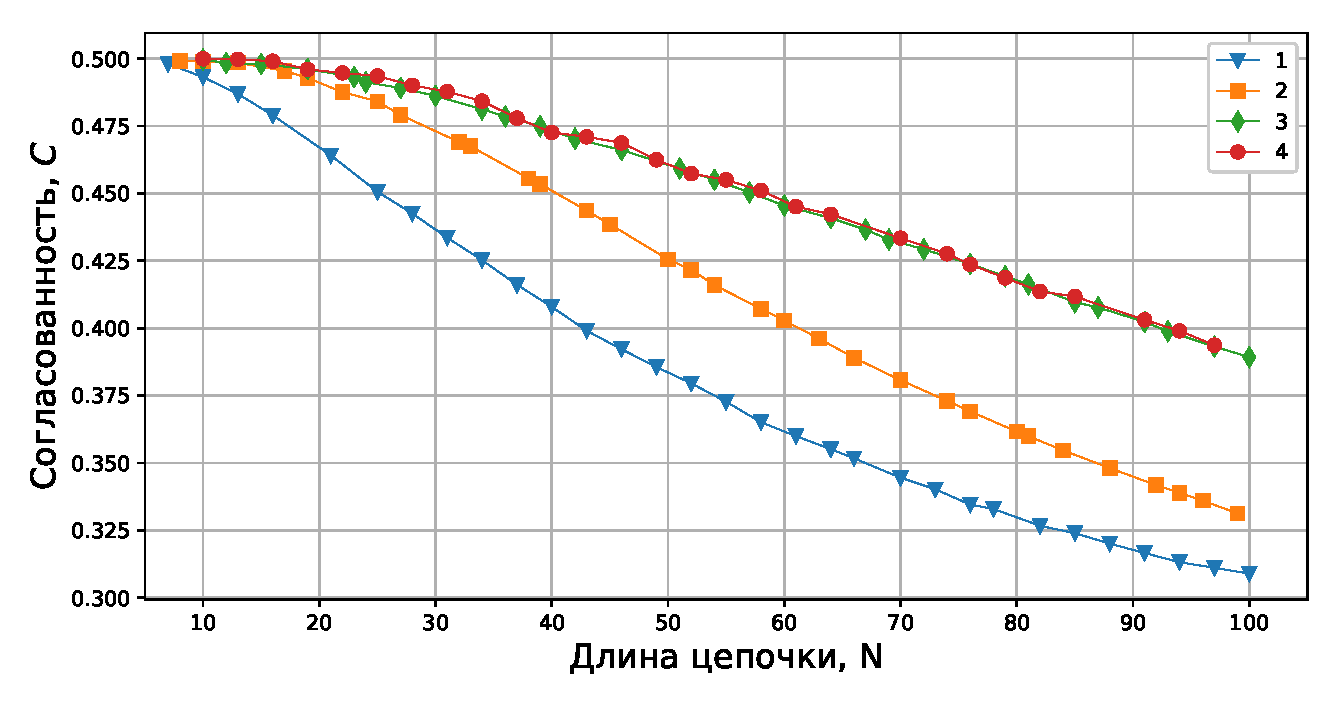
\includegraphics[width=0.9\textwidth]{concurence-n-s3.eps}
    \caption{
      Максимальное значение согласованности второго и третьего спинов передатчика, состояние которого может быть передано без потерь,
      от количества узлов в цепи.
      Разные линии отвечают разным размерам расширенного приемника.
    }
    \label{fig:concurence-n-s3}
\end{figure}


Так как элементы матрицы плотности, вносящие вклад в каждую когерентность, перемешиваются в процессе эволюции,
на расширенном приемнике ER применятся специальное унитарное преобразование $U^\mathrm{ER}(\phi)$ для их распутывания~\cite{Feldman2017}.
По аналогии с работой~\cite{Bochkin2022} можно подобрать такое унитарное преобразование на расширенном приемнике,
которое позволяет передавать состояния с максимальным значением согласованности второго и третьего спинов передатчика.
На Рис.~\ref{fig:concurence-n-s3} приведены максимально возможные значения согласованности от длины цепочки,
полученные путем максимизации модуля недиагонального элемента $\omega$ матрицы плотности $\rho^\mathrm{S}_\mathrm{init}$ по параметрам унитарного преобразования $U^\mathrm{ER}(\phi)$.
Вычисления выполнены с помощью метода дифференциальной эволюции~\cite{Storn1997,Wormington1999,Lampinen2002} из библиотеки SciPy~\cite{SciPy} версии 1.4.1.


\section{Зигзагообразная цепочка}

\begin{wrapfigure}{O}{0.5\textwidth}
    \centering
    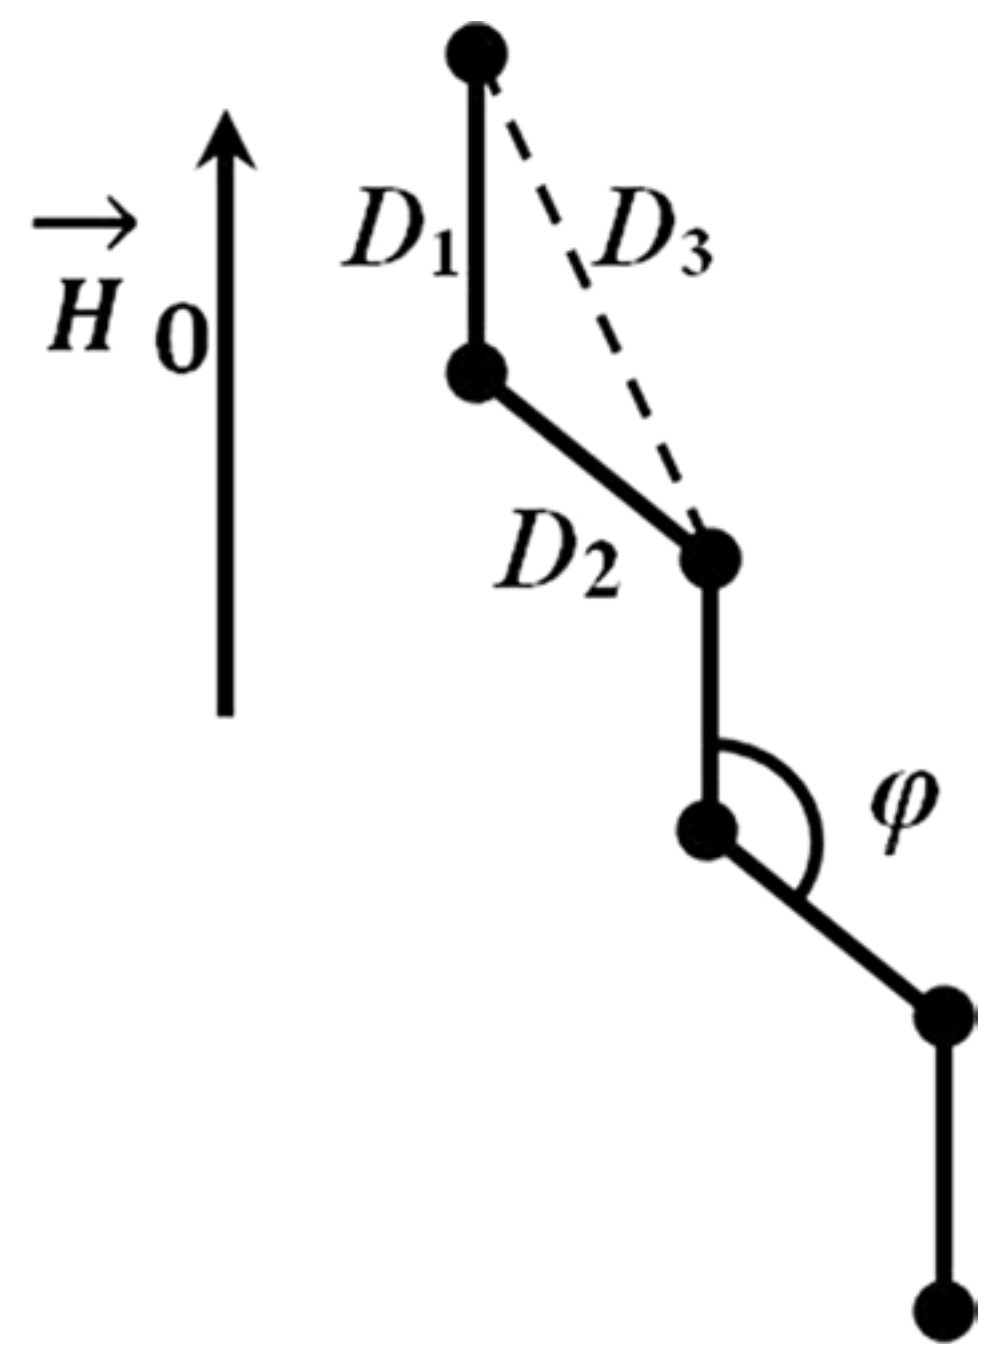
\includegraphics[width=0.3\textwidth]{model-zchain-schema}
    \caption{\protectСхема зигзагообразной цепочки ядерных спинов.
Нечетные звенья параллельны внешнему магнитному полю $\vec{H}_0$,
а $\varphi$ --- угол между соседними звеньями.
% Константы связи $D_1$ и $D_2$ определяются уравнением~(\ref{eq:dipolaconstantsnearest}), а $D_3=D_{n, n+2},\, (n=1,2,...)$
% уравнением~(\ref{eq:dipolaconstantsnextnearest}).
}
    \label{fig:model-zchain-schema}
\end{wrapfigure}

В зигзагообразных цепочках в кристалле гамбергита в МК эксперименте ЯМР,
в отличие от однородных цепочек,
существенны когерентности плюс/минус четвертого порядка (см. раздел~\ref{sec:model-zigzag-chain}).
Данное обстоятельство является важным для исследования многоспиновой запутанности,
поскольку при этом используется второй момент распределения МК когерентностей ЯМР.

На Рис.~\ref{fig:model-zchain-schema} схематично представлена
зигзагообразная цепочка ядерных спинов в сильном внешнем магнитном поле $\vec{\mathcal H}_0$.
Нечетные звенья цепочки параллельны внешнему магнитному полю $\vec{\mathcal H}_0$,
а $\varphi$ - угол между соседними звеньями.
гамильтониан $\hmq$,
описывающий МК динамику ЯМР~(см. раздел~\ref{sec:mq-nrm-experiment}),
задается выражением~\cite{Doronin2000}
%
\begin{equation}\label{hmq-next-nearest}
  \hmqZChainNextNearest = \hmqZChainNextNearestDefinition,
\end{equation}
%
\hmqZChainNextNearestExplanatoryNote
%
Константы диполь-дипольного взаимодействия (ДДВ)
в зигзагообразной цепочке определяются выражениями~\cite{Abragam1982}
%
\begin{equation}\label{eq:dipolaconstantsnearest}
  D_{2n-1, 2n} = D_1 =\dfrac{\gamma^2\hbar }{r^3},
  \quad
  D_{2n, 2n+1} = D_2=\dfrac{\gamma^2\hbar }{2r^3}\p{3\cos^2 \varphi -1},
  \quad
  n=1,2\dots,
\end{equation}
где $\gamma$ -- гиромагнитное отношение,
и $r$ -- расстояние между ближайшими спинами в цепочке.
Также в гамильтониане учитываются взаимодействия со следующими соседями,
константа диполь-дипольного взаимодействия которых определяется как~\cite{Abragam1982}
%
\begin{equation}\label{eq:dipolaconstantsnextnearest}
  D_{n, n+2}=\dfrac{\gamma^2\hbar }{16r^3 \sin^3 \frac{\varphi}{2}}\p{3\sin^2 \frac{\varphi}{2} -1}.
\end{equation}
%
В частности, уравнения~(\ref{eq:dipolaconstantsnearest}),~(\ref{eq:dipolaconstantsnextnearest}) означают,
что для прямой спиновой цепочки, когда  $(\varphi=\pi)$,
константа дипольной связи для ближайших соседей в восемь раз больше,
чем константа дипольной связи между следующими ближайшими соседями.
Тем не менее при $\varphi=\frac{2\pi}{3}$ отношение констант связи
\begin{equation}
  \left|\dfrac{D_{2n, 2n+1}}{D_{2n-1, 2n+1}}\right| = \dfrac{3\sqrt{3}}{5},
\end{equation}
и, следовательно,
диполь-дипольные взаимодействия следующих ближайших соседей
существенны для МК динамики ЯМР при определённых ориентациях зигзагообразной спиновой цепочки
по отношению к направлению внешнего сильного магнитного поля.


\subsection{Температурная зависимость многочастичной запутанности}

\begin{figure}[H]
  \begin{subfigure}[t]{0.31\textwidth}
    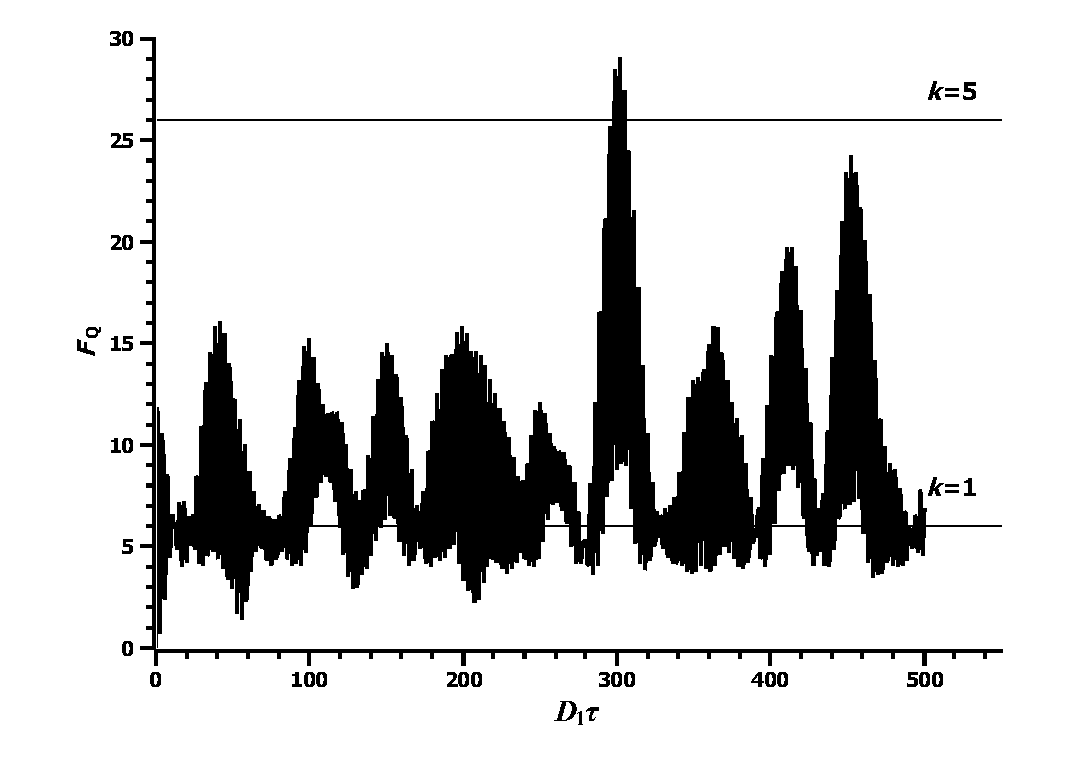
\includegraphics[width=\textwidth]{result-zchain-m2-by-time-n6-beta10}
    \caption{\protect$\beta=10$ ($T = 2.4\times 10^{-3}$~К), $N=6$.
В области выше горизонтальной линии $k=1$ детектируется парная запутанность, выше $k=5$ --- шестиспиновая запутанность.
}
    \label{fig:result-zchain-m2-by-time-n6-beta10}
  \end{subfigure}
  \hfill
  \begin{subfigure}[t]{0.32\textwidth}
    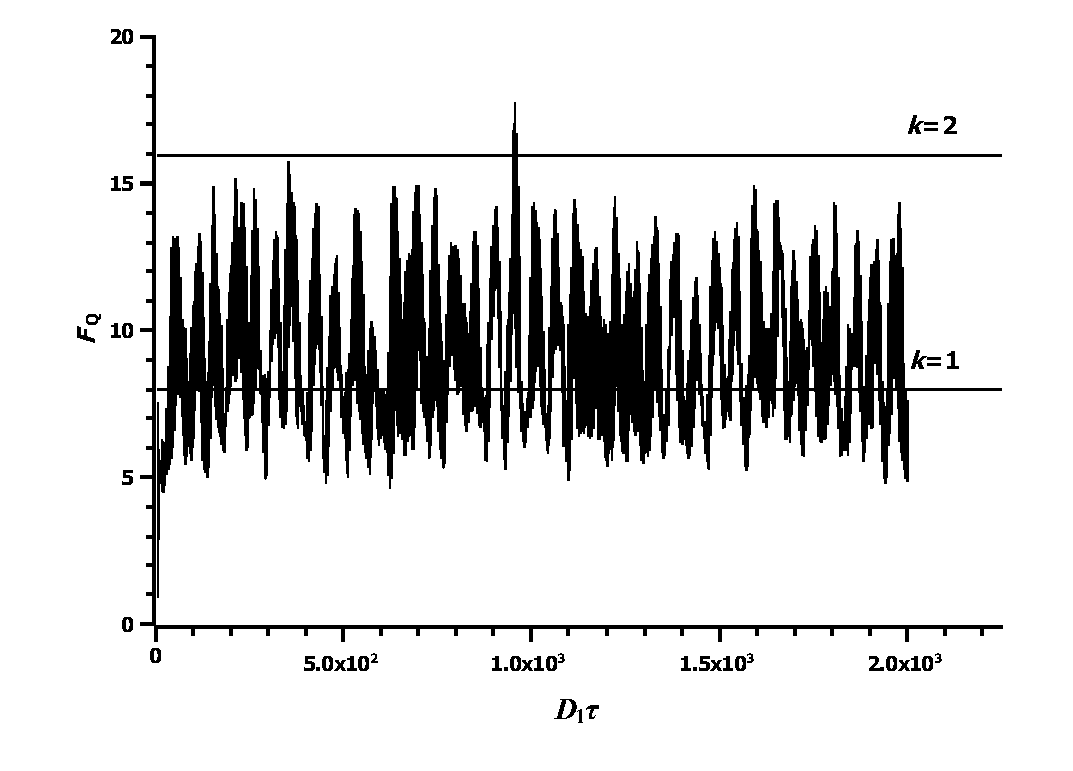
\includegraphics[width=\textwidth]{result-zchain-m2-by-time-n8-beta1}
    \caption{\protect$\beta = 1$ ($T = 2.4\times 10^{-2}$~К), $N=8$.
В области ограниченной горизонтальными линиями $k=1$ и $k=2$
детектируется парная запутанность.
}
    \label{fig:result-zchain-m2-by-time-n8-beta1}
  \end{subfigure}
  \hfill
  \begin{subfigure}[t]{0.31\textwidth}
    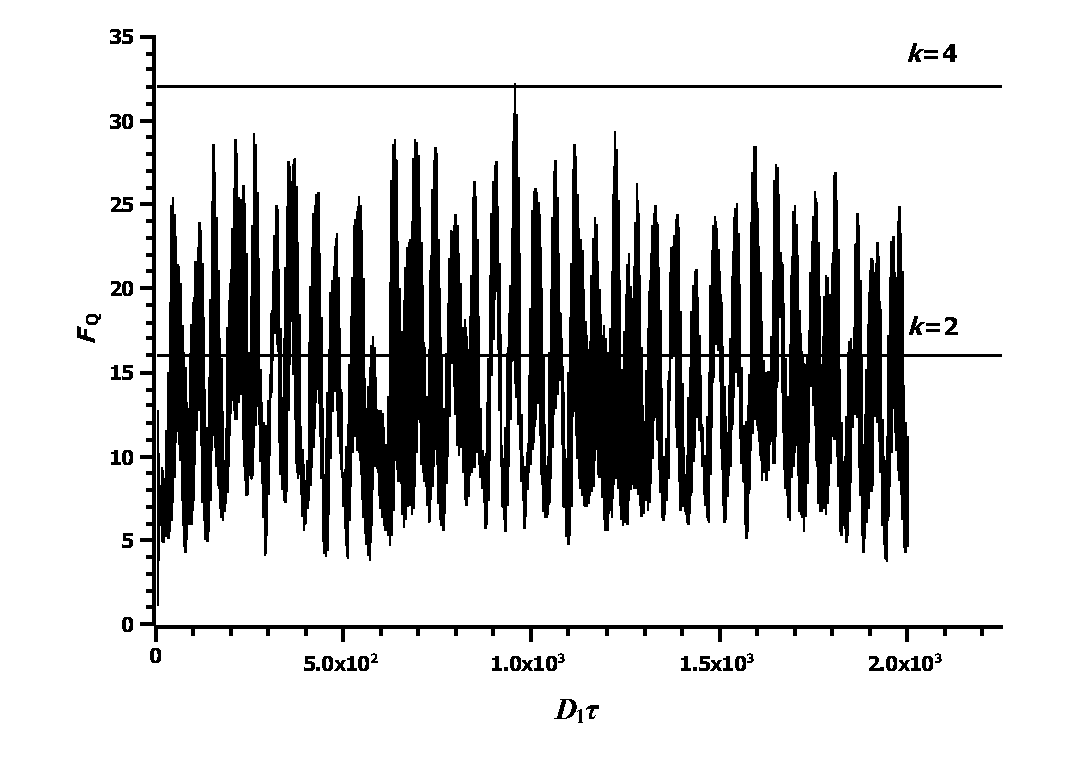
\includegraphics[width=\textwidth]{result-zchain-m2-by-time-n8-beta20}
    \caption{\protect$\beta = 20$ ($T = 1.2\times 10^{-3}$~К), $N=8$.
В области ограниченной горизонтальными линиями $k=2$ и $k=4$
детектируется трехчастичная запутанность.
}
    \label{fig:result-zchain-m2-by-time-n8-beta20}
  \end{subfigure}
  \caption{\protectЗависимость нижней границы квантовой информации Фишера~$F_Q=2M_2(\tau, \beta)$
от безразмерного времени~$D_1\tau$
в зигзагообразной цепочке.
% Горизонтальные линии соответствуют максимальным значениям информации Фишера $k$-разделимых состояний.}
  \label{fig:result-zchain-m2-by-time-ns-betas}
\end{figure}

Для исследования температурной зависимости многочастичной запутанности
в зигзагообразных цепочках
в этом разделе будет рассмотрена МК динамика ЯМР
на подготовительном периоде МК эксперимента ЯМР~(см. раздел~\ref{sec:mq-nrm-experiment})
с начальным термодинамическим равновесным состоянием $\rho_\mathrm{eq}$.
Матрица плотности системы в начальный момент времени имеет вид:
\begin{equation}
  \rho(0, \beta)
  = \rho_\mathrm{eq}
  = \dfrac{e^{\frac{\hbar\omega_{0}}{kT} I_z}}{Z},
  = \dfrac{e^{\beta I_z}}{Z},
\end{equation}
где $Z = \tr{e^{\beta I_z}}$ --- статистическая сумма,
$\hslash$ и $k$ --- константы Планка и Больцмана,
$\omega_{0}$ --- частота Лармора,
$I_\mathrm{z}$ ---  оператор проекции полного углового спинового момента  на ось~$z$,
который направлен вдоль сильного внешнего магнитного поля.

Интенсивности приведенных МК когерентностей ЯМР определяются уравнением~(\ref{eq:reduced-mq-coherences})~(см. раздел~\ref{sec:reduced-mq-coherences}).
Для $\beta=0.5$,
что соответствует температуре $T=4.8 \times 10^{-2}\,\mbox{K}$
при Ларморовской частоте $\omega_0=2\pi\times 500\times 10^6 \,\mbox{s}^{-1}$,
было обнаружено,
что неравенство~(\ref{eq:entanglement-criteria}) может быть выполнено только при $k=1$ для спиновых цепочек с $N=6$ и $N=8$.
Это означает, что в высокотемпературном случае~\cite{Doronin2019}
детектируется парная запутанность,
что согласуется с работой~\cite{Feldman2012}.

% \begin{figure}[H]
%   \begin{subfigure}[t]{0.49\textwidth}
%     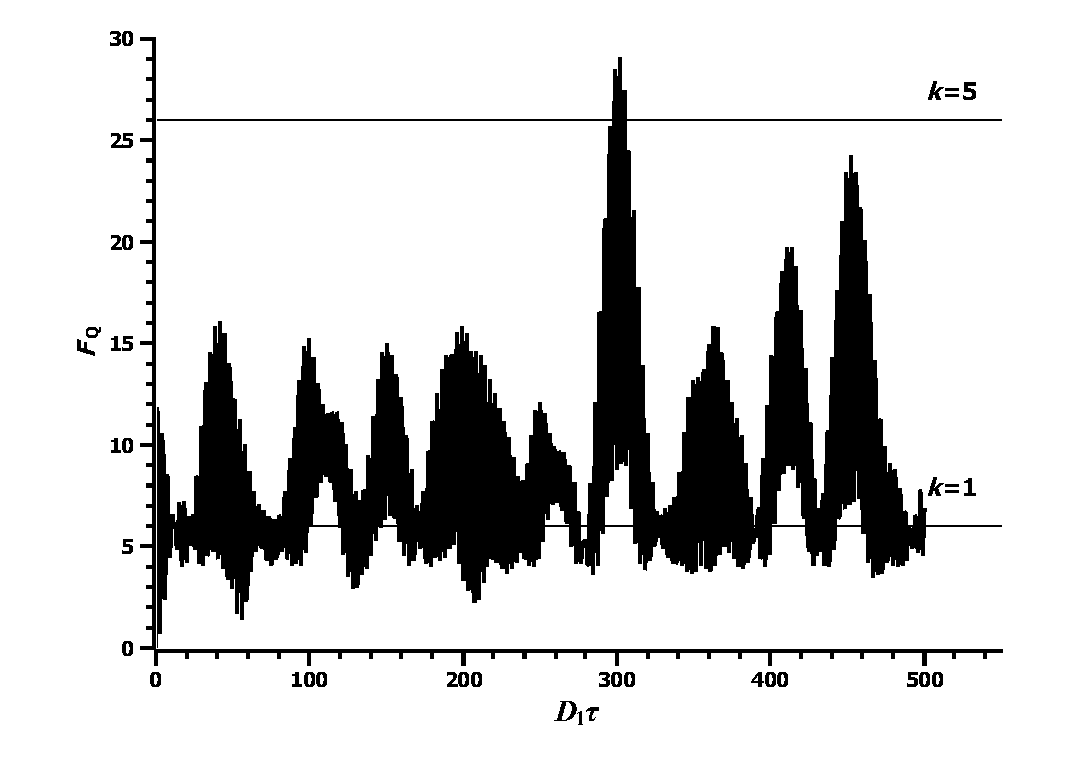
\includegraphics[width=\textwidth]{result-zchain-m2-by-time-n6-beta10}
%     \caption{
%       Зависимость нижней границы квантовой информации
%       Фишера~$F_Q=2M_2(\tau, T)$
%       от безразмерного времени~$D_1\tau$
%       для зигзагообразной цепочки из 6 спинов
%       при температуре $2.4\times 10^{-3}\,\mbox{K}$ $(b=10)$.
%       В области выше горизонтальной линии $k=1$
%       гарантировано существует как минимум парная запутанность.
%       В области выше горизонтальной линии $k=5$
%       гарантировано существует шестиспиновая запутанность.
%     }
%     \label{fig:result-zchain-m2-by-time-n6-beta10}
%   \end{subfigure}
%   \hfill
%   \begin{subfigure}[t]{0.49\textwidth}
%     
\includegraphics[width=\textwidth]{result-zchain-nent-by-n-beta10}
%     \caption{
%       Зависимость оценки максимального количества запутанных спинов $N_{ent}$ от длины цепочки при температуре $2.4\times 10^{-3}\,\mbox{K}$.
%     }
%     \label{fig:result-zchain-nent-by-n-beta10}
%   \end{subfigure}
%   \caption{}
% \end{figure}

Зависимости многоспиновой запутанности от длины цепочки $N$ и температуры исследованы для спиновых цепочек с $4\leqslant N \leqslant 12$.
Временная эволюция нижней границы квантовой информации Фишера,
соответствующая  удвоенному второму моменту распределения интенсивностей МК когерентностей для шестиспиновой цепочки представлена на Рис.~\ref{fig:result-zchain-m2-by-time-n6-beta10} при температуре $2.4\times 10^{-3}\,\mbox{K}$ $(\beta=10)$.
На Рис.~\ref{fig:result-zchain-m2-by-time-n6-beta10} видна полоса,
в которой неравенство~(\ref{eq:entanglement-criteria}) может быть удовлетворено при $1\leqslant k \leqslant 5$.
Таким образом, существует многоспиновая запутанность в спиновых кластерах, состоящих из 2-6 спинов при температуре $2.4\times 10^{-3}\,\mbox{K}$.
Зависимость оценки максимального количества запутанных спинов от длины цепи приведена на Рис.~\ref{fig:result-zchain-nent-by-n-beta10} при температуре $2.4\times 10^{-3}\,\mbox{K}$.

% \begin{figure}[H]
%   \begin{subfigure}[t]{0.49\textwidth}
%     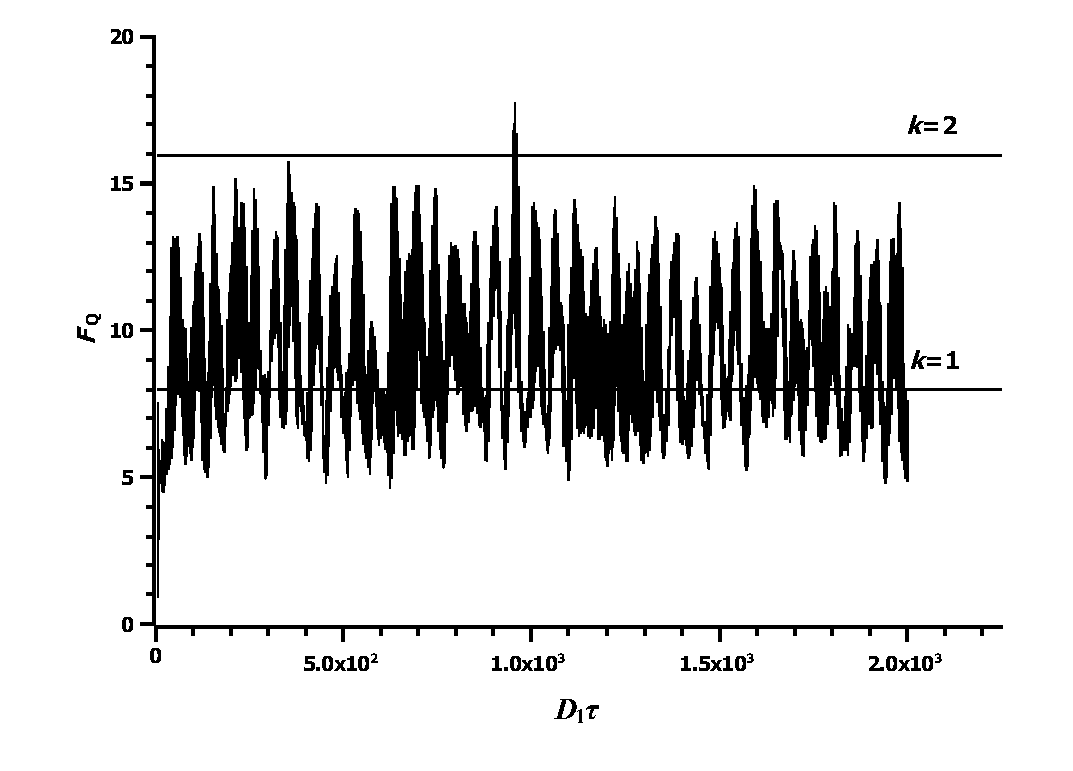
\includegraphics[width=\textwidth]{result-zchain-m2-by-time-n8-beta1}
%     \caption{
%       При температуре $2.4\times 10^{-2}\,\mbox{K}$
%       в области ограниченной горизонтальными линиями $k=1$ и $k=2$
%       присутствует как минимум парная запутанность.
%     }
%     \label{fig:result-zchain-m2-by-time-n8-beta1}
%   \end{subfigure}
%   \hfill
%   \begin{subfigure}[t]{0.49\textwidth}
%     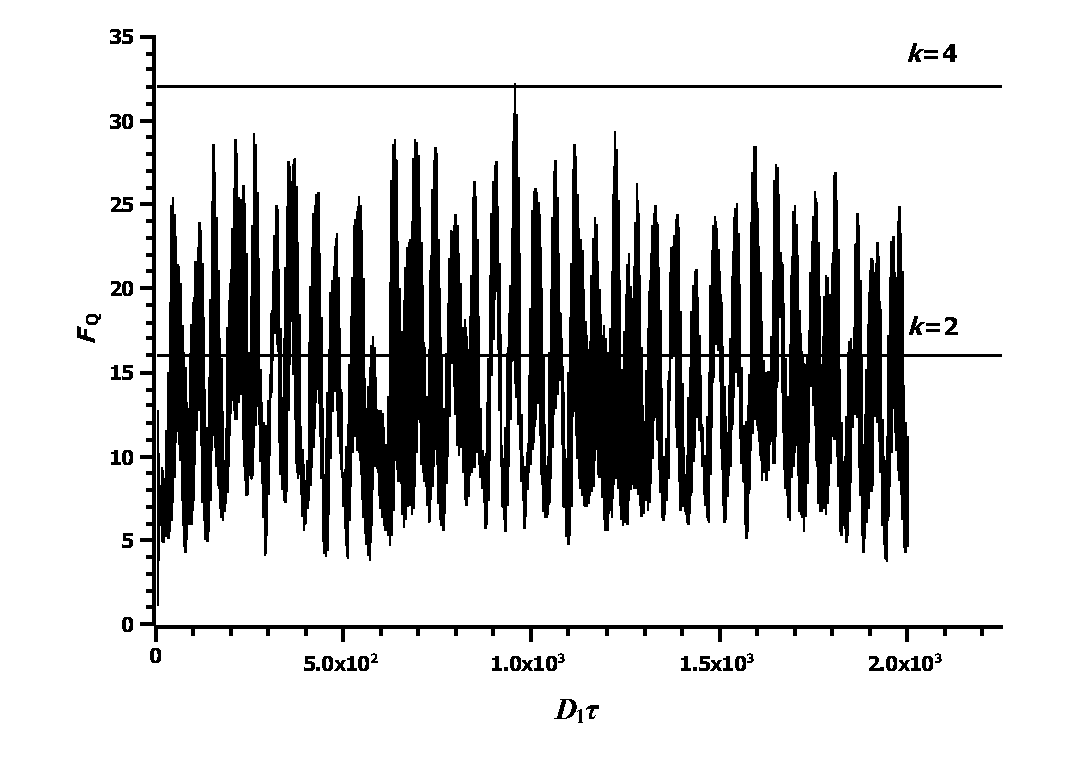
\includegraphics[width=\textwidth]{result-zchain-m2-by-time-n8-beta20}
%     \caption{
%        При температуре $1.2\times 10^{-3}\,\mbox{K}$
%        в области ограниченной горизонтальными линиями $k=2$ и $k=4$
%        наблюдается как минимум трехчастичная запутанность.
%     }
%     \label{fig:result-zchain-m2-by-time-n8-beta20}
%   \end{subfigure}
%   \caption{
%     Временная эволюция нижней границы информации Фишера~$F_Q=2M_2(\tau, T)$
%     от безразмерного времени~$D_1\tau$
%     в восьмиспиновой зигзагообразной цепочке.
%   }
% \end{figure}


\begin{figure}[H]
  \begin{subfigure}[t]{0.48\textwidth}
    \centering
    
\includegraphics[width=\textwidth]{result-zchain-nent-by-n-beta10}
    \caption{}
    % \caption{\protectЗависимость максимального задетектированного размера запутанного кластера~$N_{ent}$ от длины цепочки $N$ при температуре $\beta = 10$ ($T = 2.4\times 10^{-3}$~К).
}
    \label{fig:result-zchain-nent-by-n-beta10}
  \end{subfigure}
  \hfill
  \begin{subfigure}[t]{0.48\textwidth}
    \centering
    
\includegraphics[width=\textwidth]{result-zchain-nent-by-beta-n8-n6}
    \caption{}
    % \caption{\protectЗависимость максимального измеренного числа запутанных спинов~$N_{ent}$ от обратной температуры $\beta$
в зигзагообразной цепочке,
состоящей из шести и восьми спинов.}
    \label{fig:result-zchain-nent-by-beta-n8-n6}
  \end{subfigure}
  \label{fig:result-zchain-nent-by-betaand-n}
  \caption{\protect Зависимость максимального числа запутанных спинов~$N_{ent}$ от
\subref{fig:result-zchain-nent-by-n-beta10}) длины зигзагообразной цепочки $N$ при температуре $\beta = 10$ ($T = 2.4\times 10^{-3}$~К);
\subref{fig:result-zchain-nent-by-beta-n8-n6}) температуры $\beta$ в зигзагообразной цепочке, состоящей из шести и восьми спинов.}
\end{figure}


% \begin{wrapfigure}{O}{0.5\textwidth}
%   \centering
%   
\includegraphics[width=0.5\textwidth]{result-zchain-nent-by-beta-n8-n6}
%   \caption{
%     Зависимость оценки максимального числа запутанных спинов от обратной температуры $b$
%     для зигзагообразной цепочки,
%     состоящей из шести и восьми спинов.
%     }
%     \label{fig:result-zchain-nent-by-beta-n8-n6}
% \end{wrapfigure}

Временная эволюция восьмиспиновой зигзагообразной цепочки представлена при $T=2.4\times 10^{-2}\,\mbox{K}$ (Рис.~\ref{fig:result-zchain-m2-by-time-n8-beta1}) и $T=1.2\times 10^{-2}\,\mbox{K}$ (Рис.~\ref{fig:result-zchain-m2-by-time-n8-beta20}).  Видно, что при температуре $T=2.4\times 10^{-2}\,\mbox{K}$ возникают многоспиновые запутанные кластеры, состоящие из двух или трех спинов, а при температуре $T=1.2\times 10^{-2}\,\mbox{K}$ возникают кластеры с $2\leqslant k \leqslant 5$.
Число запутанных спинов увеличивается с понижением температуры.

Зависимость числа запутанных спинов от температуры для зигзагообразных цепочек,
состоящих из шести или восьми спинов, приведена на Рис.~\ref{fig:result-zchain-nent-by-beta-n8-n6}.
% В этих цепочках почти все спины запутаны при низких температурах.
Так же как и в случае системы эквивалентных спинов,
при низких температурах почти все спины в цепочке запутанны.
% Результаты получены на небольшом интервале времени,
% поэтому эффектами декогеренции можно пренебречь.


% The creation of entangled clusters in the considered zigzag chains is limited by weak DDIs of remote spins.  Accordingly, that process requires a large time interval. Practically, the role of decoherence gets very important in that case.  We note also that the analysis of the inequality \eqref{inequalityforfq} shows that an increase in chain length does not result in an increase of the number of the entangled spins even at long times. Indeed, we can rewrite \eqref{inequalityforfq} in the approximate simple form
% \begin{equation}\label{inequalityforfq2}
% F_Q>k N.
% \end{equation}
% In order to estimate the Fisher information we use the Gaussian approximation for the distribution of the intensities of MQ coherences \cite{baum}
% \begin{equation}\label{gaussaprox}
% J(\tau, T)=\dsfrac{1}{\sqrt{\pi N_c(T)}} \exp\p{{-\frac{n^2}{N_c(T)}}},
% \end{equation}
% where $N_c(T)$ is the number of the correlated spins which are responsible for the creation of the MQ coherence profile. Since twice the second moment $2M_2(\tau, T)$ is a lower bound on the quantum Fisher information $F_Q$ \cite{toth, pezze} one can find from Eq. \eqref{gaussaprox} that
% \begin{equation}\label{qfisheinf}
% F_Q=N_c(T).
% \end{equation}
% Since $N\geqslant N_c(T)$, one can conclude that in the Gaussian model \cite{baum} only two-spin entanglement is possible.
%
% Numerical calculations for the zigzag spin chain yield similar results. We find that the Fisher information depends only weakly on the number of spins. It means (see Eq. \eqref{inequalityforfq2}) that the number of the entangled spins decreases when $N$ increases. We have found that in the zigzag six-spin system all six spins can be entangled. On the contrary, only three spins are entangled in the zigzag ten-spin system.
%
% Finally, the number of the entangled spins for the zigzag chain with $4\leqslant N\leqslant 12$ increases with decreasing temperature.


\section{Выводы}
В этом разделе была исследована многочастичная запутанность,
возникающая на подготовительном периоде МК эксперимента ЯМР
в зигзагообразной цепочке ядерных спинов.
Несмотря на то, что в одномерных системах
создание запутанных кластеров ограничено слабыми ДДВ удаленных спинов,
удалось показать что качественное поведение температурной зависимости многочастичной запутанности
в зигзагообразной цепочке совпадает с поведением в системе эквивалентных спинов.
%Несмотря на то, что одномерные системы демонстрируют
%более скромные оценки количества запутанных частиц
%из-за отсутствия сильных дальнодействующих связей,
%можно заключить,
%что качественное поведение температурной зависимости многочастичной запутанности
%совпадает с поведением в системе эквивалентных спинов.
Более того, полученные результаты исследования запутанности
соответствуют результатам, представленным в литературе.
Таким образом, можно заключить,
что разработанный в данной диссертации метод
является мощным инструментом для исследования многочастичной запутанности в любой системе.

\chapter{Измерение информации Вигнера-Янасе в МК эксперименте ЯМР}
\label{chapter:wyi-mesuarement}

% PLA-2021

В разделе~\ref{sec:manyparticle-entanglement-criteria} был обсужден критерий многочастичной запутанности
в терминах обобщенной информации.
В свою очередь в разделах~\ref{sec:quantum-fisher-information}~и~\ref{sec:skew-wigner-yanase-information}
было показано,
что в качестве такой обобщённой меры информации могут выступать
квантовая информация Фишера и косая информация Вигнера-Янасе.
Тем не менее в прошлых разделах многочастичная запутанность была исследована исключительно
на основе квантовой информации Фишера.
Главной причиной такого выбора является тот факт,
что нижняя граница квантовой информации Фишера может быть измерена в МК эксперимента ЯМР~(см.  раздел~\ref{sec:quantum-fisher-information-mesuarement-at-high-temperature}),
и, следовательно, многочастичная запутанность может быть исследована экспериментально.
В этой главе будет продемонстрировано,
что и косая информация Вигнера-Янасе связана с
со вторым моментом МК спектра ЯМР,
а также проведено сравнение оценок многоспиновой запутанности
на основе косой информации Вигнера-Янаса и квантовой информации Фишера.



\section{Связь косой информации и второго момента МК спектра ЯМР}
\label{sec:wyi-mesuarement}

Для прояснения связи косой информации Вигнера-Янаса и
второго момента интенсивностей МК когерентностей ЯМР,
ниже будет получено выражение для косой информации
на подготовительном периоде МК эксперимента ЯМР~(см. раздел~\ref{sec:mq-nrm-experiment})
с начальным термодинамически равновесным состоянием $\rho_\mathrm{eq}$.
Матрица плотности системы в начальный момент времени имеет вид:
\begin{equation}
  \rho(0, \beta)
  = \rho_\mathrm{eq}
  = \dfrac{e^{\frac{\hbar\omega_{0}}{kT} I_z}}{Z},
  = \dfrac{e^{\beta I_z}}{Z},
\end{equation}
где $Z = \tr{e^{\beta I_z}}$ --- статистическая сумма,
$\hslash$ и $k$ --- константы Планка и Больцмана,
$\omega_{0}$ --- частота Лармора,
$I_\mathrm{z}$ ---  оператор проекции полного углового спинового момента  на ось~$z$,
который направлен вдоль сильного внешнего магнитного поля.
Эволюционная матрица плотности $\rho(\tau,\beta)$ на подготовительном периоде
под действием стационарного гамильтониана $H_\mathrm{MQ}$
может быть получена из уравнения Лиувилля,
которое имеет вид
%
\begin{equation}\label{eq:rho-eval}
  \rho(\tau,\beta)
  = V^+(\tau) \rho(0, \beta) V(\tau)
  = V^+(\tau) \frac{e^{\beta I_z}}{Z} V(\tau),
\end{equation}
где $V(\tau) = e^{iH_\mathrm{MQ}\tau}$
--- это оператор эволюции.

Косая информация Вигнера-Янасе определяется выражением~(см. раздел~\ref{sec:skew-wigner-yanase-information})
%
\begin{equation}\label{eq:wyi}
  I_{WY}(\rho(\tau,\beta),I_z)
  = -\frac{1}{2} Tr([\sqrt{\rho(\tau,\beta)},\sigma_z])^2
  = -2 Tr([\sqrt{\rho(\tau,\beta)},I_z])^2,
\end{equation}
%
где $\sigma_z=2I_z$ --- это оператор Паули.
Интригующей особенностью определения косой информации Вигнера-Янасе
является наличие корня из матрицы плотности.
Корень из матрицы плотности $\rho(\tau,\beta)$ определяется выражением
%
\begin{equation}\label{eq:rho-eval-sqrt}
  \sqrt{\rho(\tau,\beta)}
  = \sqrt{V^+(\tau)\frac{e^{\beta I_z}}{Z}V(\tau)}
  = V^+(\tau) \frac{e^{\frac{\beta}{2}I_z}}{\sqrt{Z}}V(\tau),
\end{equation}
которое может быть проверено простым вычислением:
\begin{equation}\label{eq:18}
   \sqrt{\rho}\sqrt{\rho}
   = V^+(\tau)\frac{e^{\frac{\beta}{2}I_z}}{\sqrt{Z}}
     V(\tau)V^+(\tau)\frac{e^{\frac{\beta}{2}I_z}}{\sqrt{Z}}V(\tau)
   = V^+(\tau)\frac{e^{\beta I_z}}{Z}V(\tau)
   = \rho(\tau,\beta).
\end{equation}
%
Выражение~(\ref{eq:rho-eval-sqrt}) для корня эволюционной матрицы плотности отражает интересное физическое свойство.
В действительности можно отказаться от корня
в выражении~(\ref{eq:wyi}) косой информации Вигнера-Янасе
и перейти к рассмотрению системы при вдвое большей температуре
с матрицей плотности $\rho\p{\tau,\frac \beta 2}$.
Для анализа вкладов отдельных МК когерентностей ЯМР в эволюционную матрицу плотности
$\rho(\tau,\frac \beta 2)$ можно представить ее в виде ряда~\cite{Feldman1996}
%
\begin{equation}\label{eq:}
  \rho\p{\tau,\frac \beta 2} = \sum_n \rho_{n}\p{\tau,\frac \beta 2},
\end{equation}
%
Тогда коммутатор в выражении~(\ref{eq:wyi}) можно переписать как
%
\begin{equation} \label{eq:19}
    \left[I_z,\sqrt{\rho(\tau,\beta)}\right]
    = \left[I_z, \sum_k \rho_k \left(\tau, \frac{\beta}{2}\right)\right]
    = \sum_k k\rho_k \left(\tau, \frac{\beta}{2}\right),
\end{equation}
%
и
%
\begin{equation} \label{eq:20}
	Tr\left[I_z,\sqrt{\rho(\tau,\beta)} \right]^2
	= Tr\left\{\sum_{k,k'}kk'
		\rho_k\left(\tau,\frac{\beta}{2}\right)
		\rho_{k'}\left(\tau,\frac{\beta}{2}\right)
	\right\}
	= \sum_k k^2 J_k\left(\tau,\frac{\beta}{2}\right).
\end{equation}
%
В итоге, получаем выражение для косой информации Вигнера-Янасе
через второй момент интенсивности МК когерентностей ЯМР
%
\begin{equation}\label{eq:wyi-via-second-moment}
    I_{WY}\left(\rho(\tau, \beta), I_z\right)
    = 2\sum_k k^2 J_k\left(\tau, \frac{\beta}{2}\right)
    = 2M_2\left(\tau, \frac{\beta}{2}\right).
\end{equation}
%
Таким образом, мы получаем важное наблюдение.
Если спиновая система исследуется с помощью МК ЯМР при температуре $T\sim\beta^{-1}$,
то косая информация Вигнера-Янаса равна удвоенному второму моменту
распределения интенсивностей когерентностей МК ЯМР при температуре $2T \sim 2\beta^{-1}$
в любой момент времени эволюции спиновой системы на подготовительном периоде МК эксперимента ЯМР.

Полученное равенство~(\ref{eq:wyi-via-second-moment}) позволяет экспериментально исследовать
косую информацию Вигнера-Янасе в МК эксперименте ЯМР.
В частности, по аналогии с квантовой информации Фишера
может быть исследована многочастичная запутанность (см. следующий раздел~\ref{sec:qfi-wyi-entanglement-comparison}).


\section{Сравнение оценок количества запутанных частиц}
\label{sec:qfi-wyi-entanglement-comparison}

В разделах~\ref{sec:quantum-fisher-information}~и~\ref{sec:skew-wigner-yanase-information} обсуждалось,
что квантовая информация Фишера и косая информация Вигнера-Янасе
могут быть независимо использованы для оценки количества запутанных частиц.
Ввиду результатов, полученных в разделах~\ref{sec:reduced-mq-coherences}~и~\ref{sec:wyi-mesuarement},
можно заключить,
что обе информации могут быть измерены в МК эксперименте ЯМР.
Более того, в отличие от квантовой информации Фишера,
косая информация Вигнера-Янасе может быть измерена точно.
Следовательно, возникает естественная мотивация провести сравнение
этих информаций в контексте исследования многочастичной запутанности.
Результаты такого сравнения представлены в данном разделе.

% \begin{figure}[H]
% 	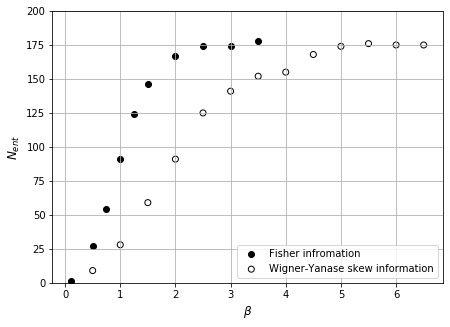
\includegraphics[width=0.95\linewidth]{nanopora_entangled_spins_by_temp}
% 	\caption{
% 		Зависимость оценки числа запутанных спинов в системе от обратной температуры $\beta = \frac{\pi \omega_0}{kT}$
% 		в нанопоре.
% 		Черные круги --- результаты полученные на основе квантовой информации Фишера.
% 		Белые круги --- результаты полученные на основе косой информации Вигнера-Янасе.
% 	}
% 	\label{fig:2}
% \end{figure}
%
% \begin{figure}[H]
% 	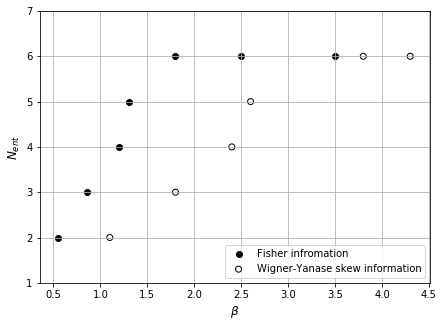
\includegraphics[width=0.95\linewidth]{zigzag_entangled_spins_by_temp}
% 	\caption{
% 		Зависимость оценки числа запутанных спинов  $N_\mathrm{ent}$
% 		от параметра обратной температуры $\beta = \frac{\pi \omega_0}{kT}$
% 		в зигзагообразной цепочке, состоящей из шести спинов.
% 		Черные круги --- результаты полученные на основе квантовой информации Фишера.
% 		Белые круги --- результаты полученные на основе косой информации Вигнера-Янасе.
% 	}
% 	\label{fig:3}
% \end{figure}

\begin{figure}[H]
  \centering
  \begin{subfigure}[t]{0.49\textwidth}
    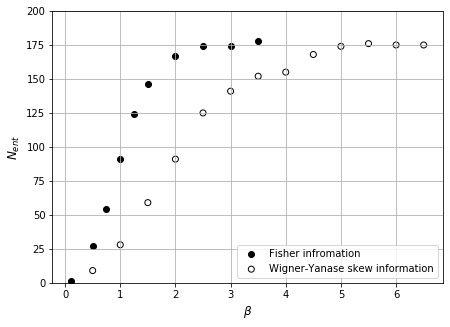
\includegraphics[width=\linewidth]{nanopora_entangled_spins_by_temp}
	\caption{
		Нанопора заполненная спин-несущими частицами.
	}
	\label{fig:qfi-wyi-comparison-nanopora}
  \end{subfigure}
  \hfill
  \begin{subfigure}[t]{0.49\textwidth}
    \includegraphics[width=\linewidth]{zigzag_entangled_spins_by_temp}
	\caption{
		Зигзагообразная цепочка, состоящей из шести спинов.
	}
	\label{fig:qfi-wyi-comparison-zigzag-chain}
  \end{subfigure}
  \caption{
    Зависимость оценки снизу числа запутанных спинов  $N_\mathrm{ent}$
	от параметра обратной температуры $\beta = \frac{\pi \omega_0}{kT}$
	Черные круги --- результаты полученные на основе квантовой информации Фишера.
	Белые круги --- результаты полученные на основе косой информации Вигнера-Янасе.
  }
  \label{fig:qfi-wyi-comparison}
\end{figure}

Величины квантовой информации Фишера~$I_\mathrm{F}(\rho(\tau,\beta),I_z)$ и косой информации Вигнера-Яанасе~$I_{WY}(\rho(\tau,\beta),I_z)$
связаны с количеством запутанных частиц в системе (см. раздел~\ref{sec:manyparticle-entanglement-criteria}).
Если величина информации превышает значение $mk^2 + (N - mk)^2$,
где $k, m$ целые числа и $m$ --- это целая часть $N/k$,
тогда гарантируется,
что в системе как минимум $k+1$ частиц связаны в одно несепарабельное состояние.

В разделе~\ref{sec:qfi-wyi-comparison} было получено следующее неравенство
для квантовой информации Фишера и косой информации Вигнера-Янасе:
%
\begin{equation} \label{eq:qfi-wyi-inequality}
    I_{WY}\left(\rho(\tau,\beta), I_z\right)
    \leq I_F\left(\rho(\tau,\beta), I_z\right)
    \leq 2I_{WY}\left(\rho(\tau,\beta), I_z\right).
\end{equation}
%
Неравенство~(\ref{eq:qfi-wyi-inequality}) позволяет надеяться,
что полученные результаты для оценки числа запутанных спинов не будут значительно отличаться.

На Рис.~\ref{fig:qfi-wyi-comparison} представлены результаты зависимости
оценки снизу количества запутанных частиц в системе от обратной температуры $\beta$.
Оценки количества запутанных частиц были полученных на основе квантовой информации Фишера и косой информации Вигнера-Янасе.
Величины обеих информаций были вычислены через второй момент распределения МК когерентностей ЯМР~(cм.
разделы~\ref{sec:reduced-mq-coherences}~и~\ref{sec:wyi-mesuarement}).
На Рис.~\ref{fig:qfi-wyi-comparison-nanopora} сравнение проведено для модели несферической нанопоры,
заполненной газом спин-несущих атомов (например, ксеноном) или молекул в сильном внешнем магнитном поле~(см. раздел~\ref{sec:model-equivalent-spins}).
Расчеты второго момента $M_2(\tau, \beta)$ были сделаны по аналогии с разделом~\ref{sec:nanopora-thermodynamic-equilibrium} для системы из 201 спина.
На Рис.~\ref{fig:qfi-wyi-comparison-zigzag-chain} сравнение проведено
для модели зигзагообразной цепочки ядерных спинов в кристалле гамбергита~(см. раздел~\ref{sec:model-zigzag-chain}).
Расчеты второго момента $M_2(\tau, \beta)$ были сделаны по аналогии с главой~\ref{chapter:manayparticle-entantlement-in-zigzag-chain}

% \section{Обобщения косой информации}
% \begin{align}
%     I_{WY}\left( \rho(t, T), I_z \right) & = 2\sum\limits_k k^2 J_k(t, 2T) = 2M_2(t, 2T) \\
%     I_{WYG}\left( \rho(t, T), I_z \right) &  = -2 \tr{\left[\rho(t, T), I_z\right]} = 2M_2(t, T) \\
%     I_{WYD} \left( \rho(t, T), I_z \right) &  = -2 \mathrm{Tr} \left\{
%         \left[\rho^\alpha, I_z \right] \left[\rho^{1 - \alpha}, I_z \right]
%     \right\}
% \end{align}

\section{Выводы}
Косая информация Вигнера-Янасе, так же как и информация Фишера,
является одной из важнейших мер в теории квантовой информации.
Полученный в этом разделе результат открывает множество возможностей
экспериментального исследования косой информации в различных системах.
В частности, она может быть применена для экспериментального исследования многочастичной запутанности.
Подобные исследования многочастичной запутанности требуют крайне низких температур $<10^{-3}$~K.
В этом случае информация Вигнера-Янасе имеет существенное преимущество перед информацией Фишера,
так как измерение первой для системы с температурой $T$
может быть проведено на установке с вдвое большей температурой $2T$.
\chapter*{Заключение}
\addcontentsline{toc}{chapter}{Заключение}

\begin{thebibliography}{}


% -- INTRODUCTION --

\bibitem{Yurishchev2011} Mikhail A. Yurishchev Phys. Rev. B 84, 024418 (2011).
\bibitem{Bera2017} A. Bera et al 2018 Rep. Prog. Phys. 81 024001 (2017).
\bibitem{Arute2019} F. Arute, R. Babbush, J. C. Bardin et al., Nature 574, 505 (2019).
\bibitem{Gisin2002} Nicolas Gisin, Grégoire Ribordy, Wolfgang Tittel, and Hugo Zbinden, Rev. Mod. Phys. 74, 145 (2002)
\bibitem{Nielsen2000} M. A. Nielsen and I. L. Chuang, Quantum Computation and Quantum Information (Cambridge University Press, 2000).
\bibitem{Yin2017} Yin, J., et al.: Satellite-based entanglement distribution over 1200 kilometers, Science 356 (6343), 1140–1144 (2017). https://doi.org/10.1126/science.aan3211
% \bibitem{Horodecki2009} Ryszard Horodecki, Pawel Horodecki, Michał Horodecki, and Karol Horodecki, Rev. Mod. Phys. 81, 865 (2009)

% Garttner2018
\bibitem{Schrodinger1935} E. Schr\"odinger, Math. Proc. Cambridge Philos. Soc. 31, 555 (1935).
% \bibitem{Hosur2016} P. Hosur, X.-L. Qi, D. A. Roberts, and B. Yoshida, J. High Energy Phys. 2016, 1 (2016).
\bibitem{DAlessio2016} L. D’Alessio, Y. Kafri, A. Polkovnikov, and M. Rigol, Adv. Phys. 65, 239 (2016).
\bibitem{Kaufman2016} A. M. Kaufman, M. E. Tai, A. Lukin, M. Rispoli, R. Schittko, P. M. Preiss, and M. Greiner, Science 353, 794 (2016).
\bibitem{Neill2016} C. Neill, P. Roushan, M. Fang, Y. Chen, M. Kolodru- betz, Z. Chen, A. Megrant, R. Barends, B. Campbell, B. Chiaro, A. Dunsworth, E. Jeffrey, J. Kelly, J. Mutus, P. J. J. O’Malley, C. Quintana, D. Sank, A. Vainsencher, J. Wenner, T. C. White, A. Polkovnikov, and J. M. Martinis, Nat. Phys. 12, 1037 (2016).
\bibitem{Doronin2003} S. I. Doronin, Phys. Rev. A 68, 052306 (2003).
\bibitem{Furman2008} G. B. Furman, V. M. Meerovich, and V. L. Sokolovsky, Phys. Rev. A 78, 042301 (2008).
\bibitem{Furman2009} G. B. Furman, V. M. Meerovich, and V. L. Sokolovsky, Quantum Inf. Process. 8, 379 (2009).
\bibitem{Feldman2008} E. B. Fel'dman and A. N. Pyrkov, JETP Lett. 88, 398 (2008).
% \bibitem{Feldman2012} E. B. Fel'dman, A. N. Pyrkov, and A. I. Zenchuk, Phil. Trans. R. Soc. A 370, 4690 (2012).

\bibitem{Alvarez2010} G. A. Alvarez and D. Suter, Phys. Rev. Lett. 104, 230403 (2010)
\bibitem{Alvarez2013} G. A. Alvarez, R. Kaiser, and D. Suter, Ann. Phys. 525,
833 (2013).
% \bibitem{Alvarez2015} G. A. Alvarez, D.Suter, and R. Kaiser, Science 349, 846 (2015)
% \bibitem{Wei2018} K. X. Wei, C. Ramanathan, and P. Cappellaro, Phys. Rev. Lett. 120, 070501 (2018)
%
\bibitem{Ball2011} Ball, P. Physics of life: The dawn of quantum biology. Nature 474, 272–274 (2011). https://doi.org/10.1038/474272a
\bibitem{Yin2007} JUAN YIN DOI: 10.1126/science.aan3211
% \bibitem{Yurishchev2011} Mikhail A. Yurishchev Phys. Rev. B 84, 024418 (2011)
\bibitem{Toth2012} G\'eza T\'oth Phys. Rev. A 85, 022322 (2012)
\bibitem{Toth2014} G. T\'oth and I. Apellaniz, J. Phys. A 47, 424006 (2014).
\bibitem{Hosur2016} P. Hosur, X.-L. Qi, D. A. Roberts, and B. Yoshida, J. High Energy Phys. 2016, 1 (2016).
\bibitem{Fan2017} R. Fan, P. Zhang, H. Shen, and H. Zhai, Science Bulletin 62, 707 (2017).

% JETP2018
\bibitem{Krojanski2004} H. G. Krojanski and D. Suter, Phys. Rev. Lett. 93, 090501 (2004).
% \bibitem{Cho2006} H. Cho, P. Cappellaro, D. G. Cory, and C. Ramana- than, Phys. Rev. B 74, 224434 (2006).
\bibitem{Bochkin2018} G. A. Bochkin, E. B. Fel’dman, S. G. Vasil’ev, and V. I. Volkov, Appl. Magn. Reson. 49, 25 (2018).

% --

\bibitem{Einstein1935} A. Einstein, B. Podolsky, and N. Rosen \textit{Phys. Rev.} \textbf{47}, 777 (1935)
\bibitem{Bell1964} J.S. Bell \textit{Physics Physique Fizika} \textbf{1}, 195 (1964)
\bibitem{Scheidl2010} T. Scheidl et al. \textit{PNAS} \textbf{107}, 46, 19708-19713 (2010)

\bibitem{Bernabeu2012} Bernabéu, J., Martínez-Vidal, F. and Villanueva-Pérez, P. J. High Energ. Phys. 2012, 64 (2012).

\bibitem{Alain1976} Alain Aspect Phys. Rev. D 14, 1944 – Published 15 October 1976

% Zeqian Chen Phys. Rev. A 71, 052302
\bibitem{Gisin1991} N. Gisin, Phys. Lett. A 154, 201 (1991).
\bibitem{Clauser1969} J. F. Clauser, M. A. Horne, A. Shimony, and R. A. Holt, Phys. Rev. Lett. 23, 880 (1969).
\bibitem{Seevinck2002} M. Seevinck and G. Svetlichny, ibid. 89, 060401 (2002).
\bibitem{Uffink2002}  J. Uffink, Phys. Rev. Lett. 88, 230406 (2002O); K. Nagata, M. Koashi, and N. Imoto, ibid. 89, 260401 (2002).
%

\bibitem{Bennett1996} C.H.Bennett et al. \textit{Phys. Rev. A} \textbf{54}, 3824 (1996)
\bibitem{Eisert2001} Eisert J. and Briegel H. J. \textit{Phys. Rev. A} \textbf{64}, 022306 (2001)
\bibitem{Wootters1998} W.K. Wootters, \textit{Phys. Rev. Lett.} \textbf{80}, 2245 (1998)


% [5 - 31] P. Hyllus et al. Phys. Rev. A 85, 022321 (2012)
\bibitem{Plenio2007} M.B. Plenio and S. Virmani, Quant. Inf. Comp. 7, 1 (2007).
\bibitem{Amico2008} L. Amico, R. Fazio, A. Osterloh, and V. Vedral, Rev. Mod. Phys. 80, 517 (2008).
\bibitem{Horodecki2009} R. Horodecki, P. Horodecki, M. Horodecki, and K. Horodecki, Rev. Mod. Phys. 81, 865 (2009).
\bibitem{Guhne2009} O. G\"uhne and G. Toth, Physics Reports 474, 1 (2009).
\bibitem{Bourennane2004} M. Bourennane, M. Eibl, C. Kurtsiefer, S. Gaertner, H. Weinfurter, O. G\"uhne, P. Hyllus, D. Bruß, M. Lewenstein, and A. Sanpera, Phys. Rev. Lett. 92, 087902
\bibitem{Kaszlikowski2008} D. Kaszlikowski and A. Kay, New. J. Phys. 10, 053026 (2008).
\bibitem{Krammer2009} P. Krammer, H. Kampermann, D. Bruß, R.A. Bertlmann, L.C. Kwek, C. Macchiavello, Phys. Rev. Lett. 103, 100502 (2009).
\bibitem{Bancal2011} J.-D. Bancal, N. Gisin, Y.-C. Liang, and S. Pironio, PRL 106, 250404 (2011).
\bibitem{Svetlichny1987} G. Svetlichny, Phys. Rev. D 35, 3066 (1987).
\bibitem{Gisin1998} N. Gisin and H. Bechmann-Pasquinucci, Phys. Lett. A 246, 1 (1998).
\bibitem{Collins2002} D. Collins, N. Gisin, S. Popescu, D. Roberts, and V. Scarani, Phys. Rev. Lett. 88, 170405 (2002).
\bibitem{Seevinck2001} M. Seevinck and J. Uffink, Phys. Rev. A 65, 012107 (2001);
\bibitem{Toth2005} G. T\'oth, O. G\"uhne, M. Seevinck, and J. Uffink, Phys. Rev. A 72, 014101 (2005).
\bibitem{Nagata2002} K. Nagata, M. Koashi, and N. Imoto, Phys. Rev. Lett. 89, 260401 (2002).
\bibitem{Yu2003} S. Yu, Z.-B. Chen, J.-W. Pan, and Y.-D. Zhang, Phys. Rev. Lett. 90, 080401 (2003)
\bibitem{Laskowski2005} W.Laskowski and M.Zukowski, Phys.Rev.A72, 062112 (2005).
\bibitem{Schmid2008} C. Schmid, N. Kiesel, W. Laskowski, W. Wieczorek, and M.Z\'ukowski,and H.Weinfurter,Phys.Rev.Lett.100, 200407 (2008).
\bibitem{Bancal2009} J.-D. Bancal, C. Branciard, N. Gisin, and S. Pironio, Phys. Rev. Lett. 103, 090503 (2009).
\bibitem{Sorensen2001} A.S. Sørensen and K. Mølmer, Phys. Rev. Lett. 86, 4431 (2001).
\bibitem{Durkin2005} G.A. Durkin and C. Simon, Phys. Rev. Lett. 95, 180402 (2005).
\bibitem{Vitagliano2011} G. Vitagliano, P. Hyllus, I.L. Egusquiza, G. T\'oth, Phys. Rev. Lett. 107, 240502 (2011).
\bibitem{Duan2011} L.-M. Duan, Phys. Rev. Lett. 107, 180502 (2011).
\bibitem{Guhne2010} O. Guhne and M. Seevinck, New J. Phys. 12, 053002 (2010).
\bibitem{Huber2010} M. Huber, F. Mintert, A. Gabriel, and B.C. Hiesmayr, Phys. Rev. Lett. 104, 210501 (2010).
\bibitem{Li2010} C.-M. Li, K. Chen, A. Reingruber, Y.N. Chen, and J.W. Pan, Phys. Rev. Lett. 105, 210504 (2010).
\bibitem{Jungnitsch2011} B. Jungnitsch, T. Moroder, and O. G\"uhne, Phys. Rev. Lett. 106, 190502 (2011).
\bibitem{Vicente2011} J.I. de Vicente and M. Huber, Phys. Rev. A 84, 062306 (2011).
\bibitem{Huber2011} M. Huber, P. Erker, H. Schimpf, A. Gabriel, and B. Hiesmayr, Phys. Rev. A 83, 040301(R) (2011).
% [44]
\bibitem{Chen2005} Z. Chen, Phys. Rev. A 71, 052302 (2005).
% [45]
\bibitem{Guhne2005} O. G\"uhne, G. T\'oth, and H. J. Briegel, New J. Phys. 7, 229 (2005);
\bibitem{Guhne2006}  O. G\"uhne and G. T\'oth, Phys. Rev. A 73, 052319 (2006).
% [46]
\bibitem{Dur1999} W. D\"ur, J.I. Cirac, and R. Tarrach, Phys. Rev. Lett. 83, 3562(1999);
\bibitem{Dur2000} W. D\"urand J. I. Cirac, Phys. Rev. A61, 042314 (2000).
% [47]
\bibitem{Peres1996} A. Peres, Phys. Rev. Lett. 77, 1413 (1996);
\bibitem{Horodecki1996} M. Horodecki, P. Horodecki, and R. Horodecki, Phys. Lett. A 223, 1 (1996).
% [48]
\bibitem{Acin2001} A. Acın, D. Bruß, M. Lewenstein, and A. Sanpera, Phys. Rev. Lett. 87, 040401 (2001).
%---


\bibitem{Zeqian2005} Zeqian Chen \textit{Phys. Rev. A} \textbf{71}, 052302 (2005)

\bibitem{Hyllus2012} P. Hyllus et al. \textit{Phys. Rev. A} \textbf{85}, 022321 (2012)


% [19] Phys. Rev. A 71, 052302 (2005)
\bibitem{Wheeler2004} J.Wheeler, in Complexity, Entropy, and Physics of Information, edited by Z.H.Zurek (Addison-Wesley, Reading, MA, 1990), pp.3-28;
\bibitem{Summhammer2004}
J.Summhammer, Int.J.Theor.Phys. 33, 171(1994);
\bibitem{Frieden2004} B.R.Frieden, Science from Fisher Information: A Unification(Cambridge University Press, Cambridge, England, 2004).

\bibitem{khitrin1997} A. Khitrin, Chem. Phys. Lett. 274, 217 (1997)

\bibitem{g_arttner2018} M. G\"arttner, P. Hauke, and A. M. Rey, Phys. Rev. Lett. 120, 040402 (2018)

\bibitem{t_oth2014} G. T\"oth and I. Apellaniz, J. Phys. A 47, 424006 (2014)

\bibitem{pezz_e2018} L. Pezz\'e, A. Smerzi, M. K. Oberthaler et al., Rev. Mod. Phys. 90, 035005 (2018).

\bibitem{liu2014} J. Liu, H.-N. Xiong, F. Song, and X. Wang, Physica A 410, 167 (20


% Quatntum Fisher Information
\bibitem{Helstrom1976} C. W. Helstrom, Quantum detection and estimation theory, Academic Press, New York, 1976.
\bibitem{Holevo1982} A. S. Holevo, Probabilistic and statistical aspects of quantum theory, North-Holland, Amsterdam, 1982.


% Wigner yanase

% 10.1103/PhysRevLett.91.180403
% [3]
\bibitem{Araki1961} H. Araki and M. M. Yanase, Phys. Rev. 120, 622 (1960). [4] M. M. Yanase, Phys. Rev. 123, 666 (1961).
% [5]
\bibitem{Ozawa1991} M. Ozawa, Phys. Rev. Lett. 67, 1956 (1991).
% [6]
\bibitem{Ozawa2002a} M. Ozawa, Phys. Rev. Lett. 88, 050402 (2002).
% [7]
\bibitem{Ozawa2002b} M. Ozawa, Phys. Rev. Lett. 89, 057902 (2002).
% [8]
\bibitem{Matsumoto1993} S. Matsumoto, Prog. Theor. Phys. 90, 35 (1993).
% [9]
\bibitem{Kakazu3469} K. Kakazu and S. Pascazio, Phys. Rev. A 51, 3469
(1995).

% Chen2005
% 10.1103/PhysRevA.71.052302
% 3
% \bibitem{Einstein1935} A. Einstein, B. Podolsky, and N. Rosen, Phys. Rev. 47, 777 (1935).
% % 4
% \bibitem{Gisin1991} N. Gisin, Phys. Lett. A 154, 201 (1991).
% % 5
% \bibitem{Clauser1969} J. F. Clauser, M. A. Horne, A. Shimony, and R. A. Holt, Phys. Rev. Lett. 23, 880 (1969).
% ��6�� D. Collins, N. Gisin, S. Popescu, D. Roberts, and V. Scarani,
% Phys. Rev. Lett. 88, 170405 ��2002��; M. Seevinck and G.
% Svetlichny, ibid. 89, 060401 ��2002��.
% ��7�� J. Uffink, Phys. Rev. Lett. 88, 230406 ��2002��; K. Nagata, M.
% Koashi, and N. Imoto, ibid. 89, 260401 ��2002��.
% ��8�� S.-X. Yu, Z.-B. Chen, J.-W. Pan, and Y.-D. Zhang, Phys. Rev.
% Lett. 90, 080401 ��2003��.
% ��9�� E. P. Wigner, Z. Phys. 133, 101 ��1952��; Physikertagung Wien
% ��Physik-Verlag, Mosbach, 1952��, p. 1.

% E. P. Wigner and M. M. Yanase, \textit{Proc. Nat. Acad. Sci. USA}, \textbf{49}, 910–918 (1963)
% [1]
\bibitem{Weaver1949} W. Weaver's article in The Mathematical Theory of Communication (Urbana: The University of IllinoisPress,1949),p.45. SeealsothelastfewpagesofM.v.Smoluchowski'sarticleinVortrage fiberdie kinetische Theorie der Materie und Elektrizit4t (Leipzig: B. G. Teubner, 1914).
% [2]
\bibitem{Wigner1960} Wigner, E. P., Z. Physik, 131, 101 (1952); Araki, H., and M. M. Yanase, Phys. Rev., 120, 622(1960).
% [3]
\bibitem{Wigner1962} Wigner,E.P.,PhysikertagungWien(Mosbach/Baden: PhysikVerlag,1962),p.1

\bibitem{Wigner1963} E. P. Wigner and M. M. Yanase, \textit{Proc. Nat. Acad. Sci. USA}, \textbf{49}, 910–918 (1963) https://www.pnas.org/doi/abs/10.1073/pnas.49.6.910

\bibitem{Luo2003prl} S. Luo, \textit{Phys. Rev. Lett.} \textbf{91}, 180403 (2003)

\bibitem{Lieb1973prl} E. H. Lieb and M. B. Ruskai, “A fundamental property of quantum-mechanical entropy,” Phys. Rev. Lett., 30, 434–436 (1973).
\bibitem{Lieb1973} E. H. Lieb, “Convex trace functions and the Wigner–Yanase–Dyson conjecture,” Adv. Math., 11, 267–288 (1973).
\bibitem{Wehrl1978} A. Wehrl, “General properties of entropy,” Rev. Modern Phys., 50, 221–260 (1978).

\bibitem{Luo2005} S. L. Luo, “Quantum versus classical uncertainty,” Theor. Math. Phys., 143, 681–688 (2005).
\bibitem{Luo2005pra} S. Luo, “Heisenberg uncertainty relation for mixed states,” Phys. Rev. A, 72, 042110 (2005).
\bibitem{Luo2006} S. Luo, “Quantum uncertainty of mixed states based on skew information,” Phys. Rev. A, 73, 022324 (2006).
\bibitem{Luo2017pra} S. Luo and Y. Sun, “Quantum coherence versus quantum uncertainty,” Phys. Rev. A, 96, 022130 (2017).

\bibitem{Luo2020} S. Luo, Theoretical and Mathematical Physics, 202(1): 104–111 (2020)
% [9-23] Luo, Theoretical and Mathematical Physics, 202(1): 104–111 (2020)
% 9.
\bibitem{Luo2012} S. Luo, S. Fu, and C. H. Oh, “Quantifying correlations via the Wigner–Yanase skew information,” Phys. Rev. A,
85, 032117 (2012).
\bibitem{Luo2003} S. Luo, Proc. Am. Math. Soc. 132 (o) (2003) 885–890.
%10.
\bibitem{Li2016a} L. Li, Q.-W. Wang, S.-Q. Shen, and M. Li, “Measurement-induced nonlocality based on Wigner–Yanase skew
information,” Europhys. Lett., 114, 10007 (2016).
%11.
\bibitem{Sun2017} Y. Sun, Y. Mao, and S. Luo, “From quantum coherence to quantum correlations,” Europhys. Lett., 118, 60007
(2017).
% 12.
\bibitem{Girolami2014} D. Girolami, “Observable measure of quantum coherence in finite dimensional systems,” Phys. Rev. Lett., 113,
170401 (2014); arXiv:1403.2446v3 [quant-ph] (2014).
% 13.
\bibitem{Yu2017} C. Yu, “Quantum coherence via skew information and its polygamy,” Phys. Rev. A, 95, 042337 (2017); arXiv:
1704.04871v1 [quant-ph] (2017).
% 14.
\bibitem{Luo2017} S. Luo and Y. Sun, “Partial coherence with application to the monotonicity problem of coherence involving skew
information,” Phys. Rev. A, 96, 022136 (2017).
% 15.
\bibitem{Luo2018} S. Luo and Y. Sun, “Coherence and complementarity in state-channel interaction,” Phys. Rev. A, 98, 012113
(2018).
% 16.
\bibitem{Karpat2014} G. Karpat, B. Cakmak, and F. F. Fanchini, “Quantum coherence and uncertainty in the anisotropic XY chain,”
Phys. Rev. B, 90, 104431 (2014); arXiv:1404.6427v3 [quant-ph] (2014).
% 17.
\bibitem{Malvezzi2016} A. L. Malvezzi, G. Karpat, B. Cakmak, F. F. Fanchini, T. Debarba, and R. O. Vianna, “Quantum correlations and coherence in spin-1 Heisenberg chains,” Phys. Rev. B, 93, 184428 (2016); arXiv:1602.03731v2 [quant-ph] (2016).
% 18.
\bibitem{Li2016b} Y.-C. Li and H.-Q. Lin, “Quantum coherence and quantum phase transitions,” Sci. Rep., 6, 26365 (2016).
% 19.
\bibitem{Lei2016} S. Lei and P. Tong, “Wigner–Yanase skew information and quantum phase transition in one-dimensional quantum spin-1/2 chains,” Quantum Inf. Process., 15, 1811–1825 (2016).
% 20.
\bibitem{Qiu2017} L. Qiu, D. Quan, F. Pan, and Z. Liu, “Skew information in the XY model with staggered Dzyaloshinskii–Moriya
interaction,” Phys. B, 514, 13–18 (2017).
% 21.
\bibitem{Yanagi2005} K. Yanagi, S. Furuichi, and K. Kuriyama, “A generalized skew information and uncertainty relation,” IEEE Trans. Inform. Theory, 51, 4401–4404 (2005).
% 22.
\bibitem{Furuichi2010} S. Furuichi, “Schrodinger uncertainty relation with Wigner–Yanase skew information,” Phys. Rev. A, 82, 034101 (2010); arXiv:1005.2655v2 [quant-ph] (2010).
% 23.
\bibitem{Chen2016} B. Chen, S.-M. Fei, and G.-L. Long, “Sum uncertainty relations based on Wigner–Yanase skew information,” Quantum Inf. Process., 15, 2639–2648 (2016); arXiv:1606.01533v1 [quant-ph] (2016).
/Furuichi2010
% 24
\bibitem{Yadin2016} B. Yadin and V. Vedral, “General framework for quantum macroscopicity in terms of coherence,” Phys. Rev. A, 93, 022122 (2016); arXiv:1505.03792v2 [quant-ph] (2015).

% mq expreimetn
% \bibitem{Baum1985} J. Baum, M. Munowitz, A. N. Garroway, and A. Pines, J. Chem. Phys. 83, 2015 (1985).


% models
\bibitem{Baugh2001}J. Baugh, A. Kleinhammes, D. Han, Q. Wang, and Y. Wu, \textit{Science} \textbf{294}, 1505 (2001).


% MQ NMR

%% Master diploma
\bibitem{vesta} Koichi Momma and Fujio Izumi. VESTA 3 for three-dimensional visualization of crystal, volumetric and morphology data. Journal of Applied Crystallography, 44(6):1272–1276, Dec 2011.

\bibitem{Elliott1994} J. C. Elliott. Structure and chemistry of the apatites and other calcium orthophosphates. Studies in Inorganic Chemistry 18. Elsevier Science, Amsterdam, 1994.

%% JETP Lett. 2015
%\bibitem{Baum1985} J. Baum, M. Munoviz, A. N. Garroway, and A. Pines. Multiple quantum dynamics in solid state NMR. The Journal of Chemical Physics, 83(5):2015– 2025, 1985.
\bibitem{Mattis1993} D. C. Mattis, The many-body problem: An encyclopedia of exactly solved models in one-dimension, World Scintific, Singapore (1993).
\bibitem{Shykind1988} D.N. Shykind, J. Baum, S.-B. Liu, A. Pines, and A. N. Garroway, J. Magn. Reson. 76, 149 (1988).
\bibitem{Rhim1971} W.-K. Rhim, A. Pines, and J. S. Waugh, Phys. Rev. B 3, 684 (1971).
\bibitem{Haberlen1969} U. Haberlen and J.S. Waugh, Phys. Rev. 185, 420 (1969).

%%
\bibitem{Bochkin2019jmr} G.A. Bochkin, E.B. Fel’dman, I.D. Lazarev, A.A. Samoilenko, S.G. Vasil’ev, Orientational dependencies of dynamics and relaxation of multiple quantum NMR coherences in one-dimensional systems, Journal of Magnetic Resonance (2019), doi: https://doi.org/10.1016/j.jmr.2019.02.004



% Quantum fisher information mesuarment

% PRA 2019
% [1] J. Baum, M. Munowitz, A. N. Garroway, and A. Pines, J. Chem. Phys. 83, 2015 (1985).
% [2] J. Baum and A. Pines, J. Am. Chem. Soc. 108, 7447 (1986).
% [3] J. Baum, K. K. Gleason, A. Pines, A. N. Garroway, and J. A. Reimer, Phys. Rev. Lett. 56, 1377 (1986).
% [4] H. G. Krojanski and D. Suter, Phys. Rev. Lett. 93, 090501 (2004).
% [5] H. J. Cho, P. Cappellaro, D. G. Cory, and C. Ramanathan, Phys. Rev. B 74, 224434 (2006).
% [6] G. A. Bochkin, E. B. Fel’dman, S. G. Vasil’ev, and V. I. Volkov, Appl. Magn. Reson. 49, 25 (2018).
% [7] C. M. Sánchez, R. H. Acosta, P. R. Levstein, H. M. Pastawski, and A. K. Chattah, Phys. Rev. A 90, 042122 (2014).
% [8] M. Munowitz, A. Pines, and M. Mehring, J. Chem. Phys. 86, 3172 (1987).
% [9] G. A. Álvarez, D. Suter, and R. Kaiser, Science 349, 846 (2015).
% [10] K. X. Wei, C. Ramanathan, and P. Cappellaro, Phys. Rev. Lett. 120, 070501 (2018).
% [11] S. I. Doronin, Phys. Rev. A 68, 052306 (2003).
% [12] G. B. Furman, V. M. Meerovich, and V. L. Sokolovsky, Phys. Rev. A 78, 042301 (2008).
% [13] G. B. Furman, V. M. Meerovich, and V. L. Sokolovsky, Quantum Inf. Process. 8, 283 (2009).
% [14] M. Horodecki, P. Horodecki, and R. Horodecki, Phys. Lett. A 223, 1 (1996).
% [15] E. B. Fel’dman and A. N. Pyrkov, JETP Lett. 88, 398 (2008).
% [16]
% \bibitem{Feldman2012} E. B. Fel’dman, A. N. Pyrkov, and A. I. Zenchuk, Philos. Trans. R. Soc. London A 370, 4690 (2012).
% [17] M. Gärttner, P. Hauke, and A. M. Rey, Phys. Rev. Lett. 120, 040402 (2018).
% [18]
% \bibitem{Toth2014} G. T\'oth and I. Apellaniz, J. Phys. A 47, 424006 (2014).
% [19]
\bibitem{Pezze2018} L. Pezz\'e, A. Smerzi, M. K. Oberthaler, R. Schmied, and P. Treutlein, Rev. Mod. Phys. 90, 035005 (2018).
% [20] E. B. Fel’dman and S. Lacelle, Chem. Phys. Lett. 253, 27 (1996).
% [21]
% \bibitem{Feldman1997} E. B. Fel'dman and S. Lacelle, J. Chem. Phys. 107, 7067 (1997).
% [22] S. I. Doronin, I. I. Maksimov, and E. B. Fel’dman, J. Exp. Theor. Phys. 91, 597 (2000).
% [23] J. Baugh, A. Kleinhammes, D. Han, Q. Wang, and Y. Wu, Science 294, 1505 (2001).
% [24] E. B. Fel’dman and M. G. Rudavets, J. Exp. Theor. Phys. 98, 207 (2004).
% [25]
\bibitem{Doronin2009} S. I. Doronin, A. V. Fedorova, E. B. Fel’dman, and A. I. Zenchuk, J. Chem. Phys. 131, 104109 (2009).
% [26]
\bibitem{Goldman1970} M. Goldman, Spin Temperature and Nuclear Magnetic Resonance in Solids (Clarendon, Oxford, 1970).
% [27] E. B. Fel’dman and S. Lacelle, J. Chem. Phys. 106, 6768 (1997).
% [28]
\bibitem{Landau3} L. Landau and E. M. Lifshitz, Quantum Mechanics: Non-Relativistic Theory (Pergamon, New York, 1977).
\bibitem{Landau5} L. Landau and E. M. Lifshitz, Statistical Physics (Elsevier Science, 1980)
% [29] A. Khitrin, Chem. Phys. Lett. 274, 217 (1997).
% [30] P. Hyllus, W. Laskowski, R. Krischek, C. Schwemmer, W. Wieczorek, H. Weinfurter, L. Pezzé, and A. Smerzi, Phys. Rev. A 85, 022321 (2012).
% [31] S.-Y. Hou, H. Li, and G.-L. Long, Sci. Bull. 62, 863 (2017).


%% Many-particle entanglement

% JETP 2020
% \bibitem{Nielsen2009}
% M.A.~Nielsen, and  I.L.~Chuang, Cambridge University Press, (2009).
%
% \bibitem{Arute2019}
% F.~Arute, R.~Babbush, J.C.~Bardin et al., Nature 574, 505–510 (2019).
%
% \bibitem{Baum1985}
% J.~Baum, M.~Munowitz, A.N.~Garroway and A.~Pines, J.~Chem.~Phys.~83, 2015–2025 (1985).
%
% \bibitem{Furman2008}
% G.B.~Furman, V.M.~Meerovich, and V.L.~Sokolovsky, Phys.~Rev.~A ~78,~042301 (2008).
%
% \bibitem{Furman2009}
% G.B.Furman, V.M.~Meerovich, and V.L.~Sokolovsky, Quantum Information Processing 8, 283–291 (2009).
%
% \bibitem{Feldman2008}
% E.B.~Fel’dman, and A.N.~Pyrkov, JETP Lett.~88,~398–401 (2008).~
%
% \bibitem{Feldman2012}
% E.B.~Fel'dman, A.N.~Pyrkov, and  A.I.~Zenchuk, Philosophical Transactions of the Royal Society A: Mathematical, Physical and Engineering Sciences~370,~4690–4712~(2012).
%
% \bibitem{G_rttner2018}
% M.~G\"arttner, P.~Hauke, and  A.M.~Rey, Phys.~Rev.~Lett.~120, 040402 (2018).
%
% \bibitem{T_th2014}
% G.~T\'oth, and I.~Apellaniz,~J Physics A: Mathematical and Theoretical~47,~424006 (2014).
%
% \bibitem{Pezz_2018}
% L.~Pezz\'e, A.~Smerzi, M.K.~Oberthaler et al., Rev.~Mod.~Phys.~90,~035005 (2018).
%
% \bibitem{Liu2014}
% J.~Liu, H.-N.~Xiong, F.~Song and X. Wang., Physica A: Statistical Mechanics and its Applications.~410,~167–173 (2014).
%
\bibitem{Khitrin1997}
A.~Khitrin, Chem.~Phys.~Lett.~274,~217–220 (1997).
%
%\bibitem{Doronin2019}
%S.I.~Doronin, E.B.~Fel'dman, and  I.D.~Lazarev,~Phys.~Rev.~A~100,~022330~(2019).
%
% \bibitem{Baugh2001}
% J.~Baugh, A.~Kleinhammes, D.~Han, and Q.~Wang  et al.~Science~294,~1505–1507 (2001).
%
% \bibitem{Doronin2009}
% S.I.~Doronin, A.V.Fedorova, E.B.~Fel’dman and A. I. Zenchuk.~J Chem.~Phys.~131,~104109~(2009).
%
\bibitem{Doronin2007a}
S.I.~Doronin, E.B.~Fel’dman, E.I.~Kuznetsova et al.~Phys.~Rev.~B~76,~144405~(2007).
%
% \bibitem{Goldman1970}
% .Goldman, Clarendon Press, (1970).
%
\bibitem{Slichter1961}
C.P.~Slichter, and  W.C.~Holton, Phys.~Rev.~122,~1701–1708~(1961).
%
\bibitem{Jeener1967}
J.~Jeener, and P.~Broekaert, Phys.~Rev.~157,232–240~(1967).
%
% \bibitem{Doronin2007b}
% S.I.~Doronin, E.B.~Fel’dman, E.I.~Kuznetsova et al.~JETP Lett.~86,~24–27 (2007).
%
\bibitem{Doronin2011}
S.I.~Doronin, E.B.~Fel’dman, and  A.I.~Zenchuk, JETP~113,~495–501 (2011).
%
\bibitem{Abragam1982}
A.~Abragam, and M.~Goldman, Clarendon Press, United Kingdom, (1982).
%
% \bibitem{Baum1986}
% J.Baum, and A.~Pines, JACS~108,~7447–7454~(1986).
%
% \bibitem{S_nchez2014}
% C.M.~S\'anchez, R.H.~Acosta, P.R.~Levstein et al.~Phys.~Rev.~A~90,~042122~(2014).
%
\bibitem{Munowitz1987}  M.~Munowitz, A.~Pines, and M.~Mehring, J Chem.~Phys.~86,~3172–3182 (1987).
%
% \bibitem{Alvarez2015} G.A.~Alvarez, D.~Suter, and R.~Kaiser, Science~349,~846–848 (2015).
%
% \bibitem{Wei2018} K.X.~Wei, C.~Ramanathan, and P.~Cappellaro, Phys.~Rev.~Lett.~120, 070501 (2018).
%
\bibitem{Feldman2004}
E.B.~Fel’dman, and M.G.~Rudavets, JETP 98,~207–219 (2004).
%
\bibitem{Feldman1996}
E.B.~Fel’dman, and S.~Lacelle, Chem.~Phys.~Lett.~253,~27–31 (1996).
%
% \bibitem{Zhang2009}
% W.~Zhang et al., Phys.~Rev.~A 80, 052323 (2009).
%
% \bibitem{Girolami2017}
% D.~Girolami, and B.~Yadin, Entropy~19,~124 (2017).
%
% \bibitem{Helstrom1976}
% C.W.~Helstrom, New York: Academic Press, (New York, 1976).
%
% \bibitem{Pezz_2009}
% L.~Pezz\'e, and A.~Smerzi, Phys.~Rev.~Lett.~102,~100401 (2009).
%
% \bibitem{Hyllus2012}
% P.~Hyllus et al., Phys.~Rev.~A~85,~022321 (2012).
%
% \bibitem{Toth2012}
% G.~T\'oth, Phys.~Rev.~A~85,~022322 (2012).


\bibitem{Doronin2000}  S.I. Doronin, I.I. Maksimov, E.B. Fel'dman, J. Exp. Theor. Phys. {\bf 91}, 597 (2000).

\bibitem{Feldman2012} E.B. Fel'dman, A.N. Pyrkov, A.I. Zenchuk, Phil. Trans. R. Soc. A {\bf 370}, 4690 (2012).

%% JMR 2020
% [1]
\bibitem{Baum1985} J. Baum, M. Munowitz, A.N. Garroway, A. Pines, J. Chem. Phys. 83 (5) (1985) 2015–2025.
% [2]
\bibitem{Hughes2004} C.E. Hughes, Prog. Nucl. Magn. Reson. Spectrosc. 45 (3–4) (2004) 301–313.
% [3]
\bibitem{Vasilev2018} S.G. Vasil’ev, V.I. Volkov, E.A. Tatarinova, A.M. Muzafarov, N.A. Sipyagina, S.A.Lermontov, J. Non-Cryst. Solids 489 (2018) 6–15.
% [4]
\bibitem{Avilova2019} I.A. Avilova, A.V. Chernyak, S.G. Vasil’ev, Appl. Magn. Resonan. 50 (12) (2019) 1419–1428.
% [5]
\bibitem{Mogami2014} Y. Mogami, S. Yamazaki, S. Matsuno, K. Matsui, Y. Noda, K. Takegoshi, Cem. Concr. Res. 66 (2014) 115–120.
% [6]
\bibitem{Krojanski2006} H.G. Krojanski, D. Suter, Phys. Rev. A 74 (6) (2006) 062319.
% [7]
\bibitem{Cho2006} H. Cho, P. Cappellaro, D.G. Cory, C. Ramanathan, Phys. Rev. B 74 (22) (2006) 224434.
% [8]
\bibitem{Bochkin}2018 G.A. Bochkin, E.B. Fel’dman, S.G. Vasil’ev, V.I. Volkov, Appl. Magn. Reson. 49 (1) (2018) 25–34.
% [9]
\bibitem{Sanchez2014} C.M. Sánchez, R.H. Acosta, P.R. Levstein, H.M. Pastawski, A.K. Chattah, Phys. Rev. A 90 (4) (2014) 042122.
% [10]
\bibitem{Alvarez2015} G.A. Álvarez, D. Suter, R. Kaiser, Science 349 (6250) (2015) 846–848.
% [11]
\bibitem{Wei2018} K.X. Wei, C. Ramanathan, P. Cappellaro, Phys. Rev. Lett. 120 (7) (2018) 070501.
% [12]
\bibitem{Garttner2018} M. G\"arttner, P. Hauke, A.M. Rey, Phys. Rev. Lett. 120 (4) (2018) 040402.
% [13]
\bibitem{Doronin2019} S.I. Doronin, E.B. Fel’dman, I.D. Lazarev, Phys. Rev. A 100 (2) (2019) 022330.
% [14]
\bibitem{Starkov2020} G.A. Starkov, B.V. Fine, Phys. Rev. B 101 (2) (2020) 024428.
% [15]
\bibitem{Zhang2009} W. Zhang, P. Cappellaro, N. Antler, B. Pepper, D.G. Cory, V.V. Dobrovitski, C. Ramanathan, L. Viola, Phys. Rev. A 80 (5) (2009) 052323.
% [16]
\bibitem{Feldman2014} E.B. Fel’dman, Appl. Magn. Reson. 45 (8) (2014) 797–806.
% [17]
\bibitem{Feldman1997} E.B. Fel’dman, S. Lacelle, J. Chem. Phys. 107 (18) (1997) 7067–7084.
% [18]
\bibitem{Hayashi1960} S. Hayashi, Nippon kagaku zassi 81 (4) (1960) 540–542.
% [19]
\bibitem{Lugt1964} W. Van der Lugt, W.J. Caspers, Physica 30 (8) (1964) 1658–1666.
% [20]
\bibitem{Cho1996} G. Cho, J.P. Yesinowski, J. Phys. Chem. 100 (39) (1996) 15716–15725.
% [21]
\bibitem{Itoh2005} K.M. Itoh, Solid State Commun. 133 (11) (2005) 747–752.
% [22]
\bibitem{Zachariasen1931} W.H. Zachariasen, Zeitschrift für Kristallographie - Crystalline Materials 76 (1) % (1931) 289–302.
% [23]
\bibitem{Zachariasen1963} W.H. Zachariasen, H.A. Plettinger, M. Marezio, Acta Crystallogr. A 16 (11) (1963) 1144–1146.
% [24]
\bibitem{Gatta2012} G.D. Gatta, J.M. Garry, B. Geoffrey, G. Alessandro, N. Fabrizio, Am. Mineral. 97 (11–12) (2012) 1891–1897.
% [25]
\bibitem{Burns1995} P.C. Burns, M. Novak, F.C. Hawthorne, Can. Mineralogist 33 (6) (1995) 1205– 1213.
% [26]
\bibitem{Bochkin2019} G.A. Bochkin, E.B. Fel’dman, I.D. Lazarev, A.A. Samoilenko, S.G. Vasil’ev, J. Magn. Reson. 301 (2019) 10–18.
% [27]
\bibitem{Abragam1961} A. Abragam, The principles of nuclear magnetism, Clarendon Press, Oxford, 1961.
% [28]
\bibitem{Carolan1971} J.L. Carolan, Chem. Phys. Lett. 12 (2) (1971) 389–391.
% [29]
\bibitem{Vleck1948} J.H. Van Vleck, Phys. Rev. 74 (9) (1948) 1168–1183.
% [30]
\bibitem{Engelsberg1973} M. Engelsberg, I.J. Lowe, J.L. Carolan, Phys. Rev. B 7 (3) (1973) 924–929.





% ---
\bibitem{Bochkin2020jmr} G.A. Bochkin, S.G. Vasil’ev, S.I. Doronin, E.I. Kuznetsova, I.D. Lazarev, E.B. Fel’dman, Appl. Magn. Reson. 51 (2020) 667–678.
\bibitem{Lazarev2019} I. D. Lazarev and  E. I. Kuznetsova, International Conference on Micro-and Nano-Electronics 2018 11022, 630-640 (2019)
\bibitem{Lazarev2020} I. D. Lazarev and E. B. Fel'dman, JETP 131(5) (2020)
\bibitem{Bochkin2022} G. A. Bochkin, E. B. Fel'dman, I. D. Lazarev, A. N. Pechen, A. I. Zenchuk,  arXiv:2201.01360 (2022)
\bibitem{Feldman2020} E. B. Fel'dman, A.N.Pechen, A.I.Zenchuk, Phys. Lett. A 413, 127605, (2022)
\bibitem{Doronin2021} S.I. Doronin, E.B. Fel’dman, I.D. Lazarev. “Multiple quantum NMR in solids as a method of determination of Wigner-Yanase skew information”, Phys. Lett. A 406, 127458, 2021.

\end{thebibliography}


\end{document}